%========= File containing the main LaTex document ========%
%                                                          %
% Copyright (C) ISI - All Rights Reserved                  %
% Proprietary                                              %
% Written by Med Hossam <med.hossam@gmail.com>, April 2016 %
%                                                          %
% @author: HEDHILI Med Houssemeddine                       %
% @linkedin: http://tn.linkedin.com/in/medhossam           %
%==========================================================%

%\documentclass[pfe]{./tpl/isipfe}
\documentclass[]{./tpl/isipfe}
\graphicspath{{./img/}}

\newtheorem{definition}{Definition}[section]

%\usepackage{hyperref}

\input{./tpl/new_commands}

% the command `\makeindex` is mandatory to create the index file main.idx
% https://tex.stackexchange.com/questions/9913/input-index-file-not-found
\makeindex


\newcommand{\tuple}[1]{\ensuremath{\langle {#1} \rangle}} 

\newcommand{\fireseq}[1]{\raisebox{-.3ex}{\ensuremath{\stackrel{\scriptstyle {#1}}{\longrightarrow}}}}

\newcommand{\Act}{\mathit{Act}}
\newcommand{\Obs}{\mathit{Obs}}
\newcommand{\UnObs}{\mathit{UnObs}}
\newcommand{\AP}{\mathit{AP}}
\newcommand{\KS}{\mathit{KS}}
\newcommand{\LKS}{\mathit{LKS}}
\newcommand{\LTS}{\mathit{LTS}}
\newcommand{\F}{\mathord{\mathsf{F}}}
\newcommand{\G}{\mathord{\mathsf{G}}}

% pre- and post- sets
\newcommand{\preset}[1]{\ensuremath{\,\!^\bullet{#1}}}
\newcommand{\postset}[1]{\ensuremath{{#1}^\bullet}}
\newcommand{\ipreset}[1]{\ensuremath{\,\!^\circ{#1}}}
\newcommand{\ipostset}[1]{\ensuremath{{#1}^\circ}}

% firing something
%\newcommand{\fireseq}[1]{\raisebox{-.3ex}{\ensuremath{\stackrel{\scriptstyle {#1}}{\longrightarrow}}}}
% Global report configuration

\newcolumntype{L}{>{\raggedright\arraybackslash}}
\newcolumntype{R}{>{\raggedleft\arraybackslash}}
\newcolumntype{C}{>{\centering\arraybackslash}}
\newcolumntype{P}[1]{>{\RaggedRight\arraybackslash}p{#1}}
\newcolumntype{Q}[1]{>{\centering\arraybackslash}p{#1}}

% Cover page
\title{Test Data Generator using LLM}
\author{Mohamed Yassine Boussabat}

\diplomaName{National Bachelor Degree in Computer Science}
\speciality{Software engineering and information systems}

% Supervisors are intentionally left empty until the final names are confirmed.
\proFramerName{}
\proFramerSpeciality{}
\academicFramerName{}
\academicFramerSpeciality{}

\companyName{LINEDATA}
\collegeYear{2025 - 2026}

\proSignSentence{J'autorise l'etudiant a faire le depot de son rapport de stage en vue d'une soutenance.}
\academicSignSentence{J'autorise l'etudiant a faire le depot de son rapport de stage en vue d'une soutenance.}

% Abstracts
\arabicAbstract{}
\arabicAbstractKeywords{}

\englishAbstract{
This final-year project was carried out within Linedata Tunisia and addresses the automation of test data preparation for the Longview front-office trade order management platform. The proposed solution is a configurable web application that generates coherent SQL-ready financial datasets for accounts, securities, prices, orders, executions, positions, models, and related entities. The system supports standalone generation without a database connection and connected generation based on read-only reference data retrieved from a Longview SQL Server instance. It is built with a React and TypeScript frontend, a NestJS backend, TypeORM-based configuration persistence, and optional Google Gemini enrichment to improve the realism of generated financial values. The result is a reusable tool that reduces manual SQL scripting effort, improves reproducibility, and helps QA teams prepare valid test scenarios more efficiently.
}

\englishAbstractKeywords{Test Data Generation, LLM, Longview, SQL Server, React, NestJS, Financial Data, Automation}

\frenchAbstract{
Ce projet de fin d'etudes a ete realise au sein de Linedata Tunisie et porte sur l'automatisation de la preparation des donnees de test pour la plateforme Longview, une solution front-office de gestion des ordres de trading. La solution proposee est une application web configurable capable de generer des jeux de donnees financiers coherents et compatibles avec SQL Server, couvrant les comptes, les titres, les prix, les ordres, les executions, les positions, les modeles et les entites associees. Le systeme prend en charge un mode autonome, sans connexion a une base de donnees, ainsi qu'un mode connecte exploitant en lecture seule des donnees de reference issues d'une instance Longview. L'application repose sur un frontend React et TypeScript, un backend NestJS, une persistance locale des configurations via TypeORM, et une integration optionnelle de Google Gemini afin d'ameliorer le realisme des valeurs generees. Ce travail permet de reduire l'effort de scripting SQL manuel, d'ameliorer la reproductibilite des scenarios de test et de faciliter le travail des equipes QA.
}

\frenchAbstractKeywords{Generation de donnees de test, LLM, Longview, SQL Server, React, NestJS, Donnees financieres, Automatisation}

\setboolean{wantToTypeCompanyAddress}{false}

\companyEmail{contact@linedata.com}
\companyTel{+216 71 185 800}
\companyFax{}
\companyAddressAR{}
\companyAddressFR{Immeuble Cleopatre Center, Bloc B, Centre Urbain Nord, 1082 Tunis, Tunisia}

% Additional packages and commands used by the report.
\usepackage{pifont}
\usepackage{svg}
\usepackage{enumitem}
\usepackage{xurl}

\newcommand{\cmark}{\ding{51}}
\newcommand{\xmark}{\ding{55}}
\newcommand{\figureplaceholder}[2]{%
  \fbox{%
    \begin{minipage}[c][#1][c]{0.92\textwidth}
      \centering
      \small\textit{#2}
    \end{minipage}%
  }%
}

\usepackage{graphicx}
\usepackage{ragged2e}
\AtBeginDocument{\justifying}

\begin{document}
    \frontmatter
    \justifying

        
%===== File containing the main cover of the document =====%
%                                                          %
% Copyright (C) ISI - All Rights Reserved                  %
% Proprietary                                              %
% Written by Med Hossam <med.hossam@gmail.com>, April 2016 %
%                                                          %
% @author: HEDHILI Med Houssemeddine                       %
% @linkedin: http://tn.linkedin.com/in/medhossam           %
%==========================================================%

%== It's advised to not modify the content of this file ===%
% To set your information, go to global_config.tex file    %
%==========================================================%

\thispagestyle{cover}%
\newgeometry{bottom=25mm,left=20mm,top=15mm,right=20mm}
\hspace{-47pt}
\begin{minipage}[l]{0.2\columnwidth}
\vspace{6mm}

\includegraphics[width=1.1\columnwidth]{img/FSTLOGO.png}\\
\end{minipage}
\hfill
\begin{minipage}[l]{0.6\columnwidth}
\centering
\footnotesize
\textbf{{TUNISIAN REPUBLIC}}\\
\vspace{1.5mm}
\textbf{{MINISTRY OF HIGHER EDUCATION \\
AND SCIENTIFIC RESEARCH}}\\
\vspace{1.5mm}
\textbf{{UNIVERSITY OF TUNIS EL MANAR}}\\
\vspace{1.5mm}
\textbf{{Faculty of Science of Tunis}}\\
\vspace{Computer Science Department}}
\end{minipage}
\hfill
\begin{minipage}[l]{0.02\columnwidth}
\end{minipage}
\hfill
\begin{minipage}[l]{0.18\columnwidth}
\vspace{6mm}

\includegraphics[width=0.9\columnwidth]{Logo_UTM}\\
\end{minipage}
\vskip1.5cm

\begin{center}
{\LARGE{\textbf{\textsc{Report End of Studies Project}}}}\\
\vskip0.5cm
\large

{\textbf{Presented in view of obtaining the title of :}}\\
\vskip2mm
{\textbf{\@diplomaName}}\\{\textbf{\@speciality}}
{}
\end{center}
\vskip0.6cm

\begin{center}
\textrm{Realized By :}\\
\vskip0.3cm
{\ifthenelse{\boolean{isBinomal}}
    {% IF TRUE
        \begin{center}
            \large\textbf{\@author}~~~~~ et ~~~~~
            \large\textbf{\@secondAuthor}
        \end{center}
    }
    {\LARGE\textbf{\@author}}% FALSE
}
\vskip12mm

\definecolor{isiBlue}{RGB}{31, 78, 121}

\begin{changemargin}{-9mm}{0cm}
\begin{minipage}[l]{1.1\columnwidth}
\begin{tcolorbox}[colframe=isiBlue,colback=white,boxrule=0pt,toprule=3pt,bottomrule=3pt,arc=0pt,top=0mm,right=0mm,left=0mm,bottom=0mm,boxsep=0.5mm]{
    \begin{tcolorbox}[colframe=isiBlue,colback=white, boxrule=0pt,toprule=1pt,bottomrule=1pt,arc=0pt,enlarge bottom by=-0.9mm, auto outer arc]
        \centering
        {\huge\textbf{\@title}}
    \end{tcolorbox}
}
\end{tcolorbox}
\end{minipage}
\end{changemargin}

\end{center}
\vskip8mm%

\begin{center}
\large
\begin{minipage}[c]{0.28\columnwidth}
Jury president : \\
Reviewer : \\
Supervised by :\\
Pedagogic advisor : 
\end{minipage}
\hfill
\begin{minipage}[c]{0.42\columnwidth}
\textbf{Mr. Mohamed Taha Bennani} \\
\textbf{Mrs. ZAMMELI Saloua}\\
\textbf{\@academicFramerName}\\
\textbf{\@proFramerName}
\end{minipage}
\hfill
\begin{minipage}[c]{0.26\columnwidth}
%\@proFramerSpeciality\\
%\@academicFramerSpeciality
\end{minipage}
\end{center}
\vskip5mm

\begin{center}
\large
Host organization: \@companyName\\
LIP6 : Laboratoire d'Informatique de Paris 6

\vskip0.4cm
%\begin{figure}[h]
%\centering
%{\color{white}{\fboxrule=2.5pt\fbox{
\includegraphics[width=0.5\columnwidth]{img/uspn.png}}}}
%\end{figure}

\vskip5mm
\noindent
\begin{minipage}[b]{0.48\linewidth}
    \centering
    
\includegraphics[height=2cm]{img/linedata.png}
\end{minipage}
\vskip5mm


\centering \fbox{
    \parbox{9cm}{ 
        \centering 
        IGL5 - N° 5225003
    }
}

\vspace*{5pt}
\end{center}

\afterpage{\blankpage}
        
        \setcounter{page}{1}
        \clearpage       
        \thispagestyle{empty}
        \vspace*{-2cm}
        \hspace*{-2.8cm}
        \noindent
        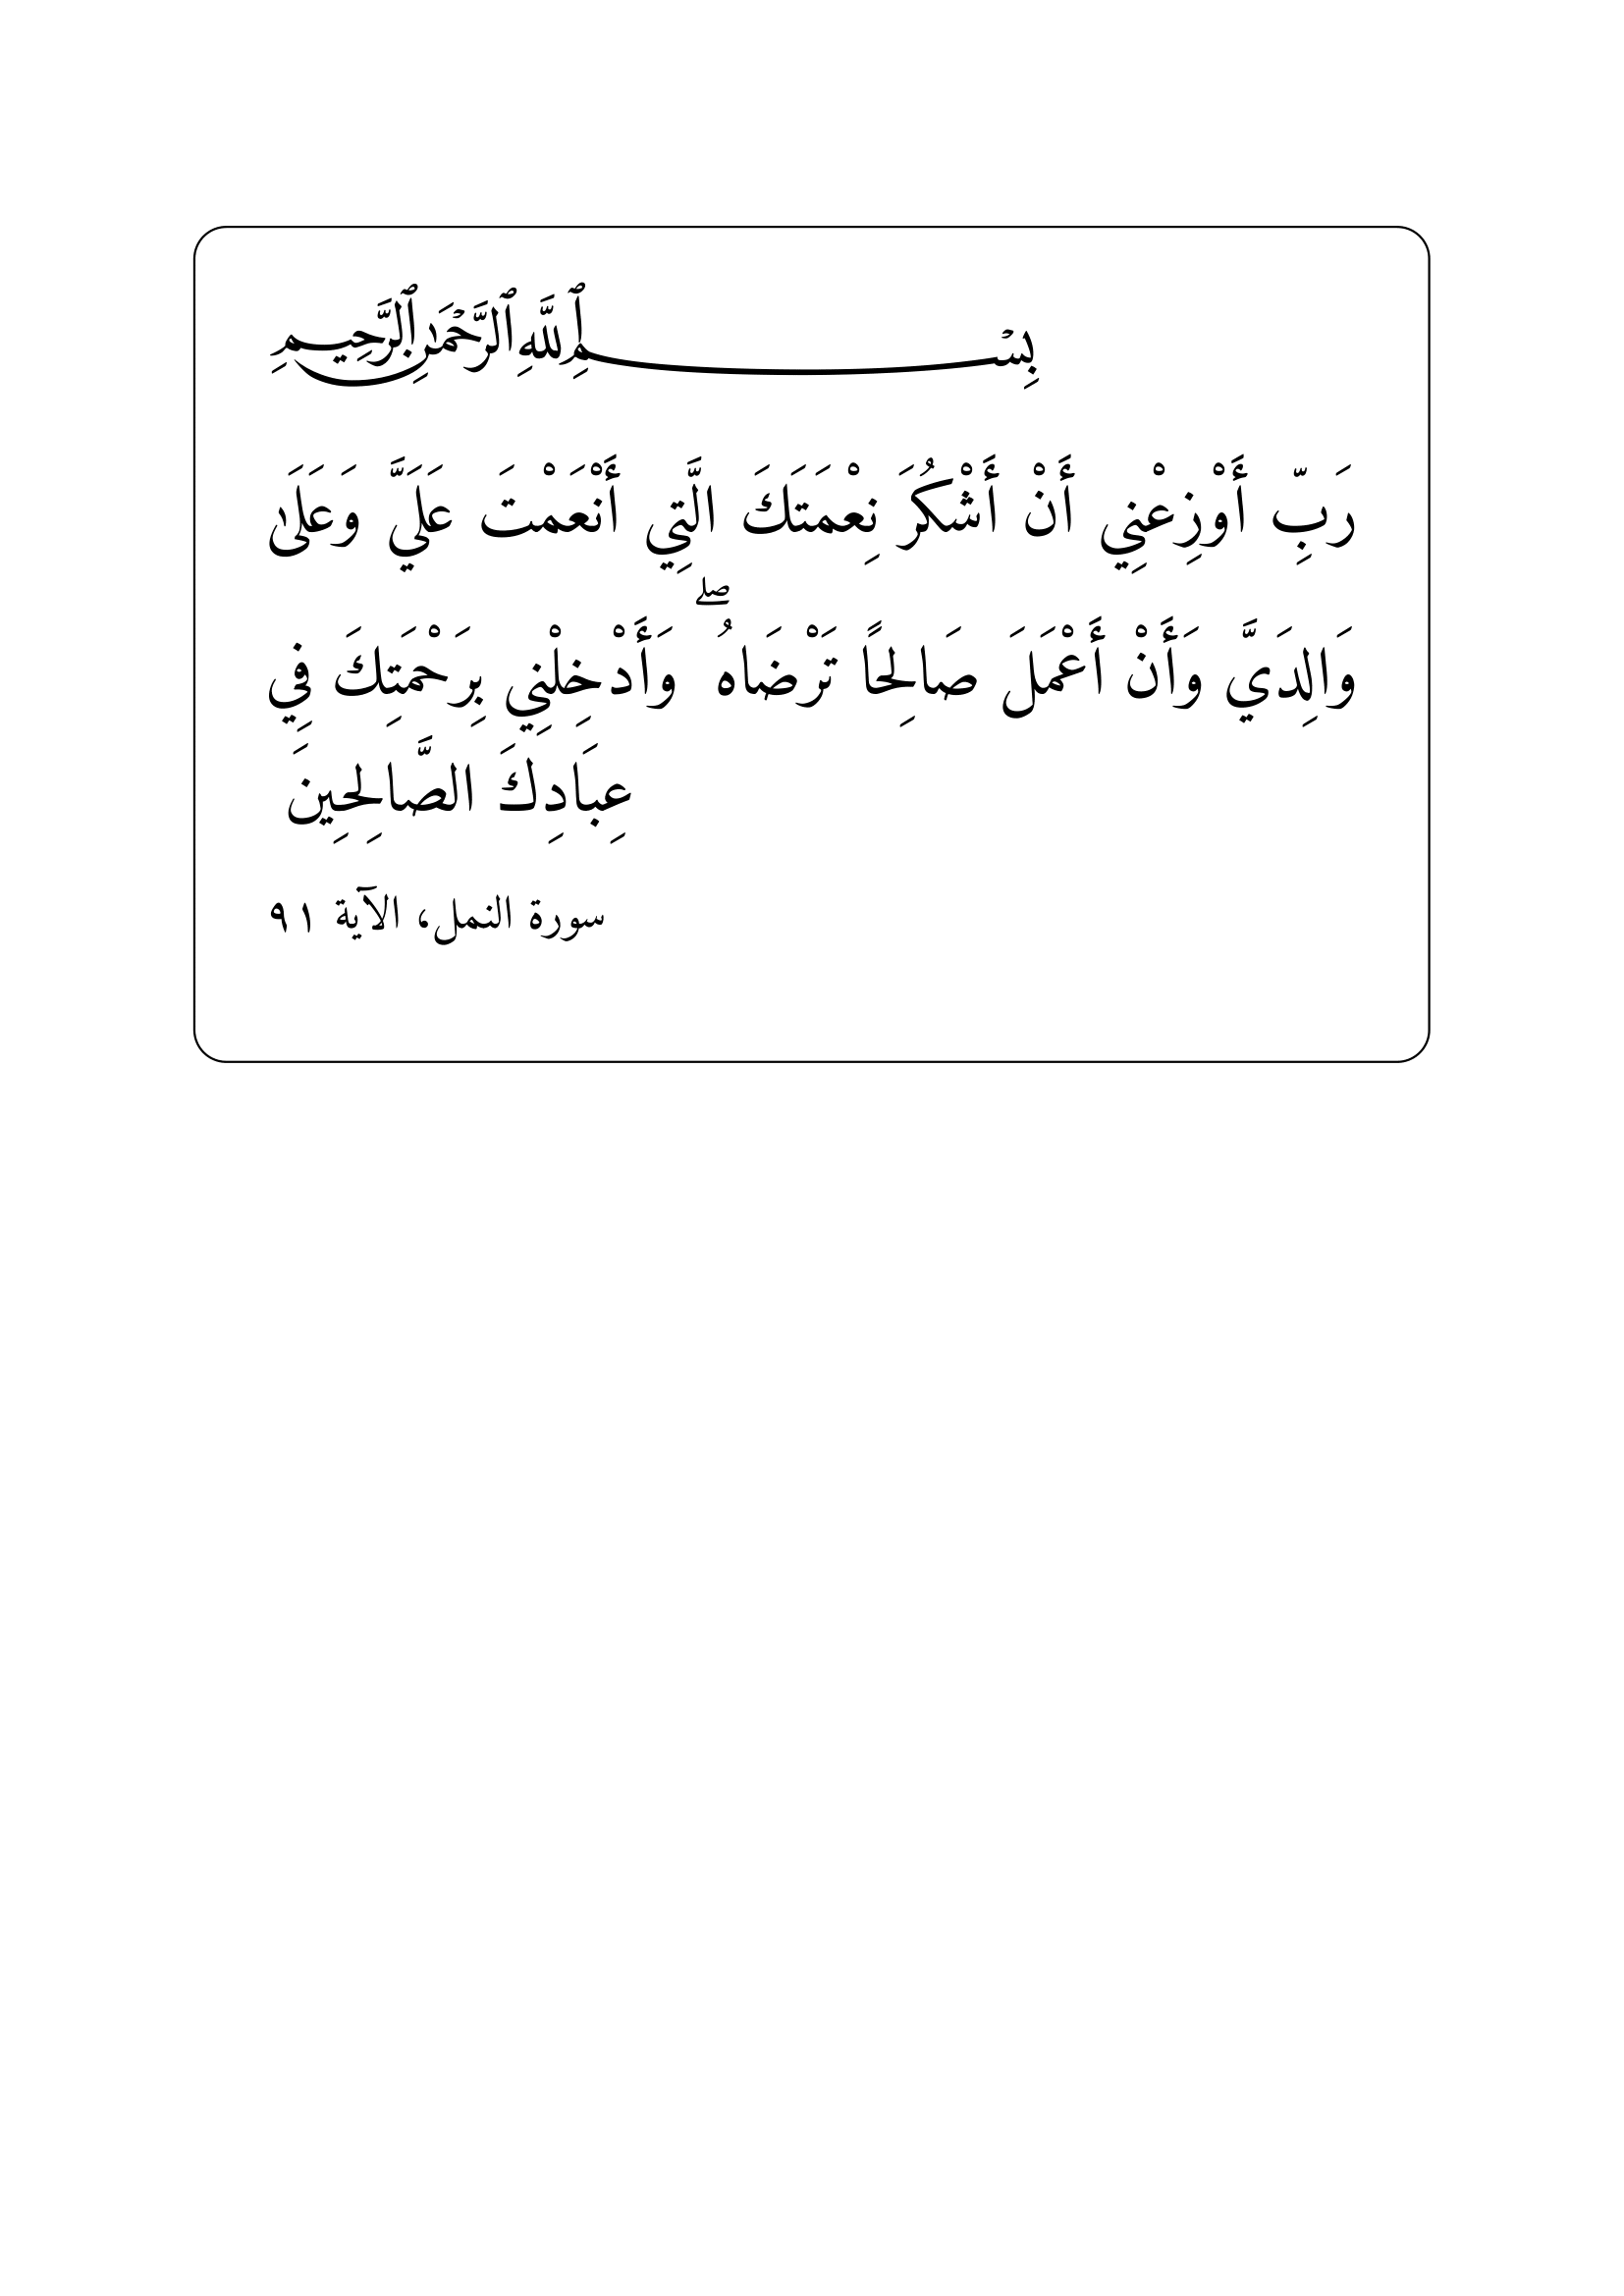
\includegraphics[width=\paperwidth,height=\paperheight]{quran-1.png}

        \chapter*{\Huge Dedication}
\begingroup
\raggedright
\setlength{\parindent}{0pt}
\setlength{\parskip}{0.25cm}

To my dearest parents, \textbf{\textit{Imen}} and \textbf{\textit{Meher}}. Your love, sacrifices, and prayers have been the foundation of everything I have achieved.

To my beloved brother, \textbf{\textit{Nizar}}. Thank you for your support, your kindness, and the strength you have always given me.

To my departed grandmother, \textbf{\textit{Turkeya}}. Your memory remains a source of tenderness, guidance, and peace in my heart.

To all my beloved \textbf{\textit{Family}}. Your encouragement and care have always made me feel surrounded and supported.

To my dear college friends, \textbf{\textit{Adem}}, \textbf{\textit{Jmal}}, \textbf{\textit{Hasni}}, \textbf{\textit{Sfar}}, \textbf{\textit{Kabil}}, \textbf{\textit{Rostom}}, \textbf{\textit{Halim}}, \textbf{\textit{Elyes}}, \textbf{\textit{Firas}}, \textbf{\textit{Mahmoud}}, \textbf{\textit{Mouath}}, \textbf{\textit{Nourhene}}, \textbf{\textit{Mayssem}}, and all the CLL community. Thank you for the shared effort, laughter, and unforgettable memories that made these university years special.

To my dear high school friends, \textbf{\textit{Iheb}}, \textbf{\textit{Haroun}}, \textbf{\textit{Abdelkdous}}, \textbf{\textit{Houssem}}, \textbf{\textit{Chahed}}, \textbf{\textit{Zahra}}, \textbf{\textit{Yassmine}}, \textbf{\textit{Yassmine}}, \textbf{\textit{Emna}}, \textbf{\textit{Sirine}}, \textbf{\textit{Sarra}}, \textbf{\textit{Nour}}, \textbf{\textit{Jasser}}, \textbf{\textit{Elyes}}, \textbf{\textit{Sana}}, \textbf{\textit{Sarra}}, and all the Sadikien community. Thank you for the sincere friendship, simple joys, and beautiful memories that still mean so much to me.

To the people who supported me during my internship period, my uncle \textbf{\textit{Mohamed}}, \textbf{\textit{Montasar}}, \textbf{\textit{Elyes}}, \textbf{\textit{Mouez}}, \textbf{\textit{Mostfa}}, and \textbf{\textit{Mohamed}}. Your help and encouragement made this important period easier and more meaningful for me.

And to all the people who have been part of my life, who have contributed in any way to my growth, my happiness, and success. Even if your name is not written here, your presence and kindness have left a mark on my journey.

This work is lovingly dedicated to all of you with deep affection, lasting respect, and infinite gratitude.

\clearpage

        \clearpage
        \thispagestyle{frontmatter}
        \chapter*{\huge Acknowledgements}
\begin{center}
\noindent
I am sincerely grateful to all those who supported and contributed to the realization of this final-year project.

First and foremost, I would like to express my deepest and most heartfelt thanks to my professional supervisor, \textbf{Mr. Souheib Baarir}, whose exceptional guidance, patience, and human warmth accompanied me throughout this journey. More than a supervisor, he was like a father to me always present, always understanding, always encouraging. His trust and unwavering support gave me the strength and confidence to move forward. I will forever be grateful for his generosity, kindness, and availability.

I would also like to thank my academic supervisor, \textbf{Mrs. Sana Younes}, for her involvement and thoughtful follow-up during the internship. Her guidance and feedback were highly appreciated.

My sincere thanks go to \textbf{Mrs. Anissa Kheireddine}, whose support and encouragement helped me during this incredible opportunity. I am truly grateful for her help and kindness.

I would like to warmly thank \textbf{Mr. Mohamed Taha Bennani} and \textbf{Mr. Kais Klai} for their trust and for believing in me from the start.

I also express my deep appreciation to the jury members: the president of the jury, \textbf{Mrs. Zouhour Ben Dhiaf}, and the reviewer of my report, \textbf{Mrs. Saloua Zammeli}, for accepting to evaluate my work. I hope this report meets their expectations in both content and clarity.

Finally, I would like to extend my gratitude to the entire teaching team of the Faculty of Sciences of Tunis for the solid academic foundation they provided, and to all those  near or far  who contributed in any way to the success of this project.

\end{center}

        \thispagestyle{frontmatter}
        
        \setcounter{secnumdepth}{3}
        \setcounter{tocdepth}{2}
        \setcounter{minitocdepth}{2}
        \dominitoc
        \tableofcontents
        \adjustmtc
        \thispagestyle{frontmatter}
        
        %\listoffigures
        %\thispagestyle{frontmatter}
        %\listoftables
        %\thispagestyle{frontmatter}
        %\listofalgorithms
        %\thispagestyle{frontmatter}
        
    \mainmatter
    \justifying

        \chapter*{General Introduction}
\addcontentsline{toc}{chapter}{General Introduction}
\markboth{General Introduction}{}

\lettrine[]{\textit{I}}{n modern financial software}, data quality plays a decisive role in the reliability of testing activities. Trading and portfolio management platforms manipulate many interdependent entities, such as accounts, securities, orders, executions, prices, and positions. Preparing coherent datasets for such systems is therefore a demanding task: every generated record must respect technical database constraints as well as financial business rules.

Within Linedata, the Longview platform is used to support front-office investment management workflows. Its quality assurance process requires realistic and reproducible datasets in order to validate new features, reproduce bugs, and run regression scenarios. However, preparing these datasets manually through SQL scripts is time-consuming, error-prone, and difficult to reuse across testing cycles. These limitations reduce productivity and make it harder to cover a wide range of financial scenarios.

The objective of this final-year project is to design and implement a configurable Test Data Generator for Longview. The proposed system provides a web interface that allows QA engineers and developers to define generation parameters without writing SQL manually. It supports standalone generation, connected generation based on existing SQL Server data, validation of generated records, configuration persistence, and optional Large Language Model enrichment to improve the realism of generated financial values.

The project was carried out using an Agile Scrum approach, with incremental sprints focused on data model discovery, generation engine implementation, connected mode implementation, LLM integration, configuration library implementation , and validation. This structure allowed the solution to evolve progressively according to technical findings and feedback from the target users.

This report is structured as follows:
\begin{itemize}
    \item \textbf{Chapter 1} presents the project context, the host organization, the Longview platform, the current test data preparation process, and the problem statement.
    \item \textbf{Chapter 2} details the requirements analysis, the selected methodology, the global architecture, the product backlog, and the technical environment.
    \item \textbf{Chapter 3} describes Sprint 1, dedicated to Longview data model discovery and the mapping of the target entities.
    \item \textbf{Chapter 4} presents Sprint 2, which delivered the core generation engine and the standalone mode.
    \item \textbf{Chapter 5} presents Sprint 3, which added SQL Server connectivity and connected generation from grabbed Longview data.
    \item \textbf{Chapter 6} presents Sprint 4, dedicated to optional Large Language Model enrichment for more realistic generated values.
    \item \textbf{Chapter 7} presents Sprint 5, which finalized the configuration library and the end-to-end application workflows.
\end{itemize}

The following chapters therefore document both the functional need behind the project and the technical decisions made to build a domain-aware tool capable of generating coherent Longview test data.

        \clearpage

        \chapter{Project Context}

% ─────────────────────────────────────────────
\section*{Introduction}
\addcontentsline{toc}{section}{Introduction}
% ─────────────────────────────────────────────

\paragraph{}This chapter presents the professional and organizational context of this internship project. It begins with an introduction to Linedata Services, the host company, followed by a description of its Tunisian office. We then provide an overview of Longview, the front-office trade management platform, covering its main functions and the key financial entities that make up its data model. The rest of the chapter examines the test data preparation methods currently used by the quality assurance and development teams, highlighting their main limitations and practical challenges. Finally, we define the core problem that motivated this project and outline the structure of the remaining chapters.

% ─────────────────────────────────────────────
\section{Host Organization: Linedata}
% ─────────────────────────────────────────────

\begin{figure}[htbp]
\centering

\includegraphics[width=0.4\textwidth]{img/linedata_logo_square.png}
\caption{Logo of Linedata \cite{linedata_about}}
\label{fig:linedata}
\end{figure}

\paragraph{}Linedata Services S.A. was founded in 1998 and has grown into a major player in the financial technology industry. The company is headquartered in Neuilly-sur-Seine, France, and operates in more than twenty offices across Europe, North America, Asia, and Africa. As of 2024, Linedata employs over 1,100 people and serves around 700 clients in 50 countries, with annual revenues exceeding \texteuro{}183 million. The company is listed on Euronext Paris under the ticker symbol LIN \cite{linedata_about, linedata_revenue}.

\paragraph{}Linedata's main goal is to make financial technology more accessible and effective by offering software platforms, data management solutions, and professional services. Its products help financial institutions such as asset managers, hedge funds, and lending organizations improve their operational efficiency, flexibility, and regulatory compliance. The company's offerings are organized into two main business segments: Asset Management and Lending \& Leasing \cite{linedata_about}.

\begin{itemize}
\item \textbf{Asset Management:} End-to-end software solutions covering portfolio management, order and execution management (OMS/EMS), investment compliance, risk analytics, and fund administration. More than 63,000 financial professionals use Linedata's asset management products every day.
\item \textbf{Lending \& Leasing:} Complete solutions for lending institutions and leasing companies, covering origination, servicing, and portfolio management.
\end{itemize}

\paragraph{}Linedata's technology is built for cloud deployment and can scale horizontally. It uses an open architecture that can connect with third-party accounting systems, trading platforms, external data providers, and custodial interfaces. The company has also been progressively integrating artificial intelligence and machine learning into its data management and analytical workflows \cite{linedata_ai}.

% ─────────────────────────────────────────────
\subsection{Linedata Tunisia}
% ─────────────────────────────────────────────

\paragraph{}The Tunisian subsidiary of Linedata plays a central role in the company's research, development, and engineering activities. Located in Tunis, the office employs software engineers, quality assurance specialists and technical leads who are responsible for the development and maintenance of Linedata's core financial platforms, particularly the Longview system.

\begin{itemize}
\item \textbf{Address:} Immeuble Cléopâtre Center, Bloc B, Centre Urbain Nord, 1082 Tunis, Tunisia
\item \textbf{Phone:} +216 71 185 800
\end{itemize}

% ─────────────────────────────────────────────
\subsection{Organizational Structure and Internship Context}
% ─────────────────────────────────────────────

\paragraph{}Engineering work at Linedata Tunisia is divided into dedicated product teams that operate under the research and development department. The internship described in this report was carried out within the Longview development team.

\begin{figure}[htbp]
\centering
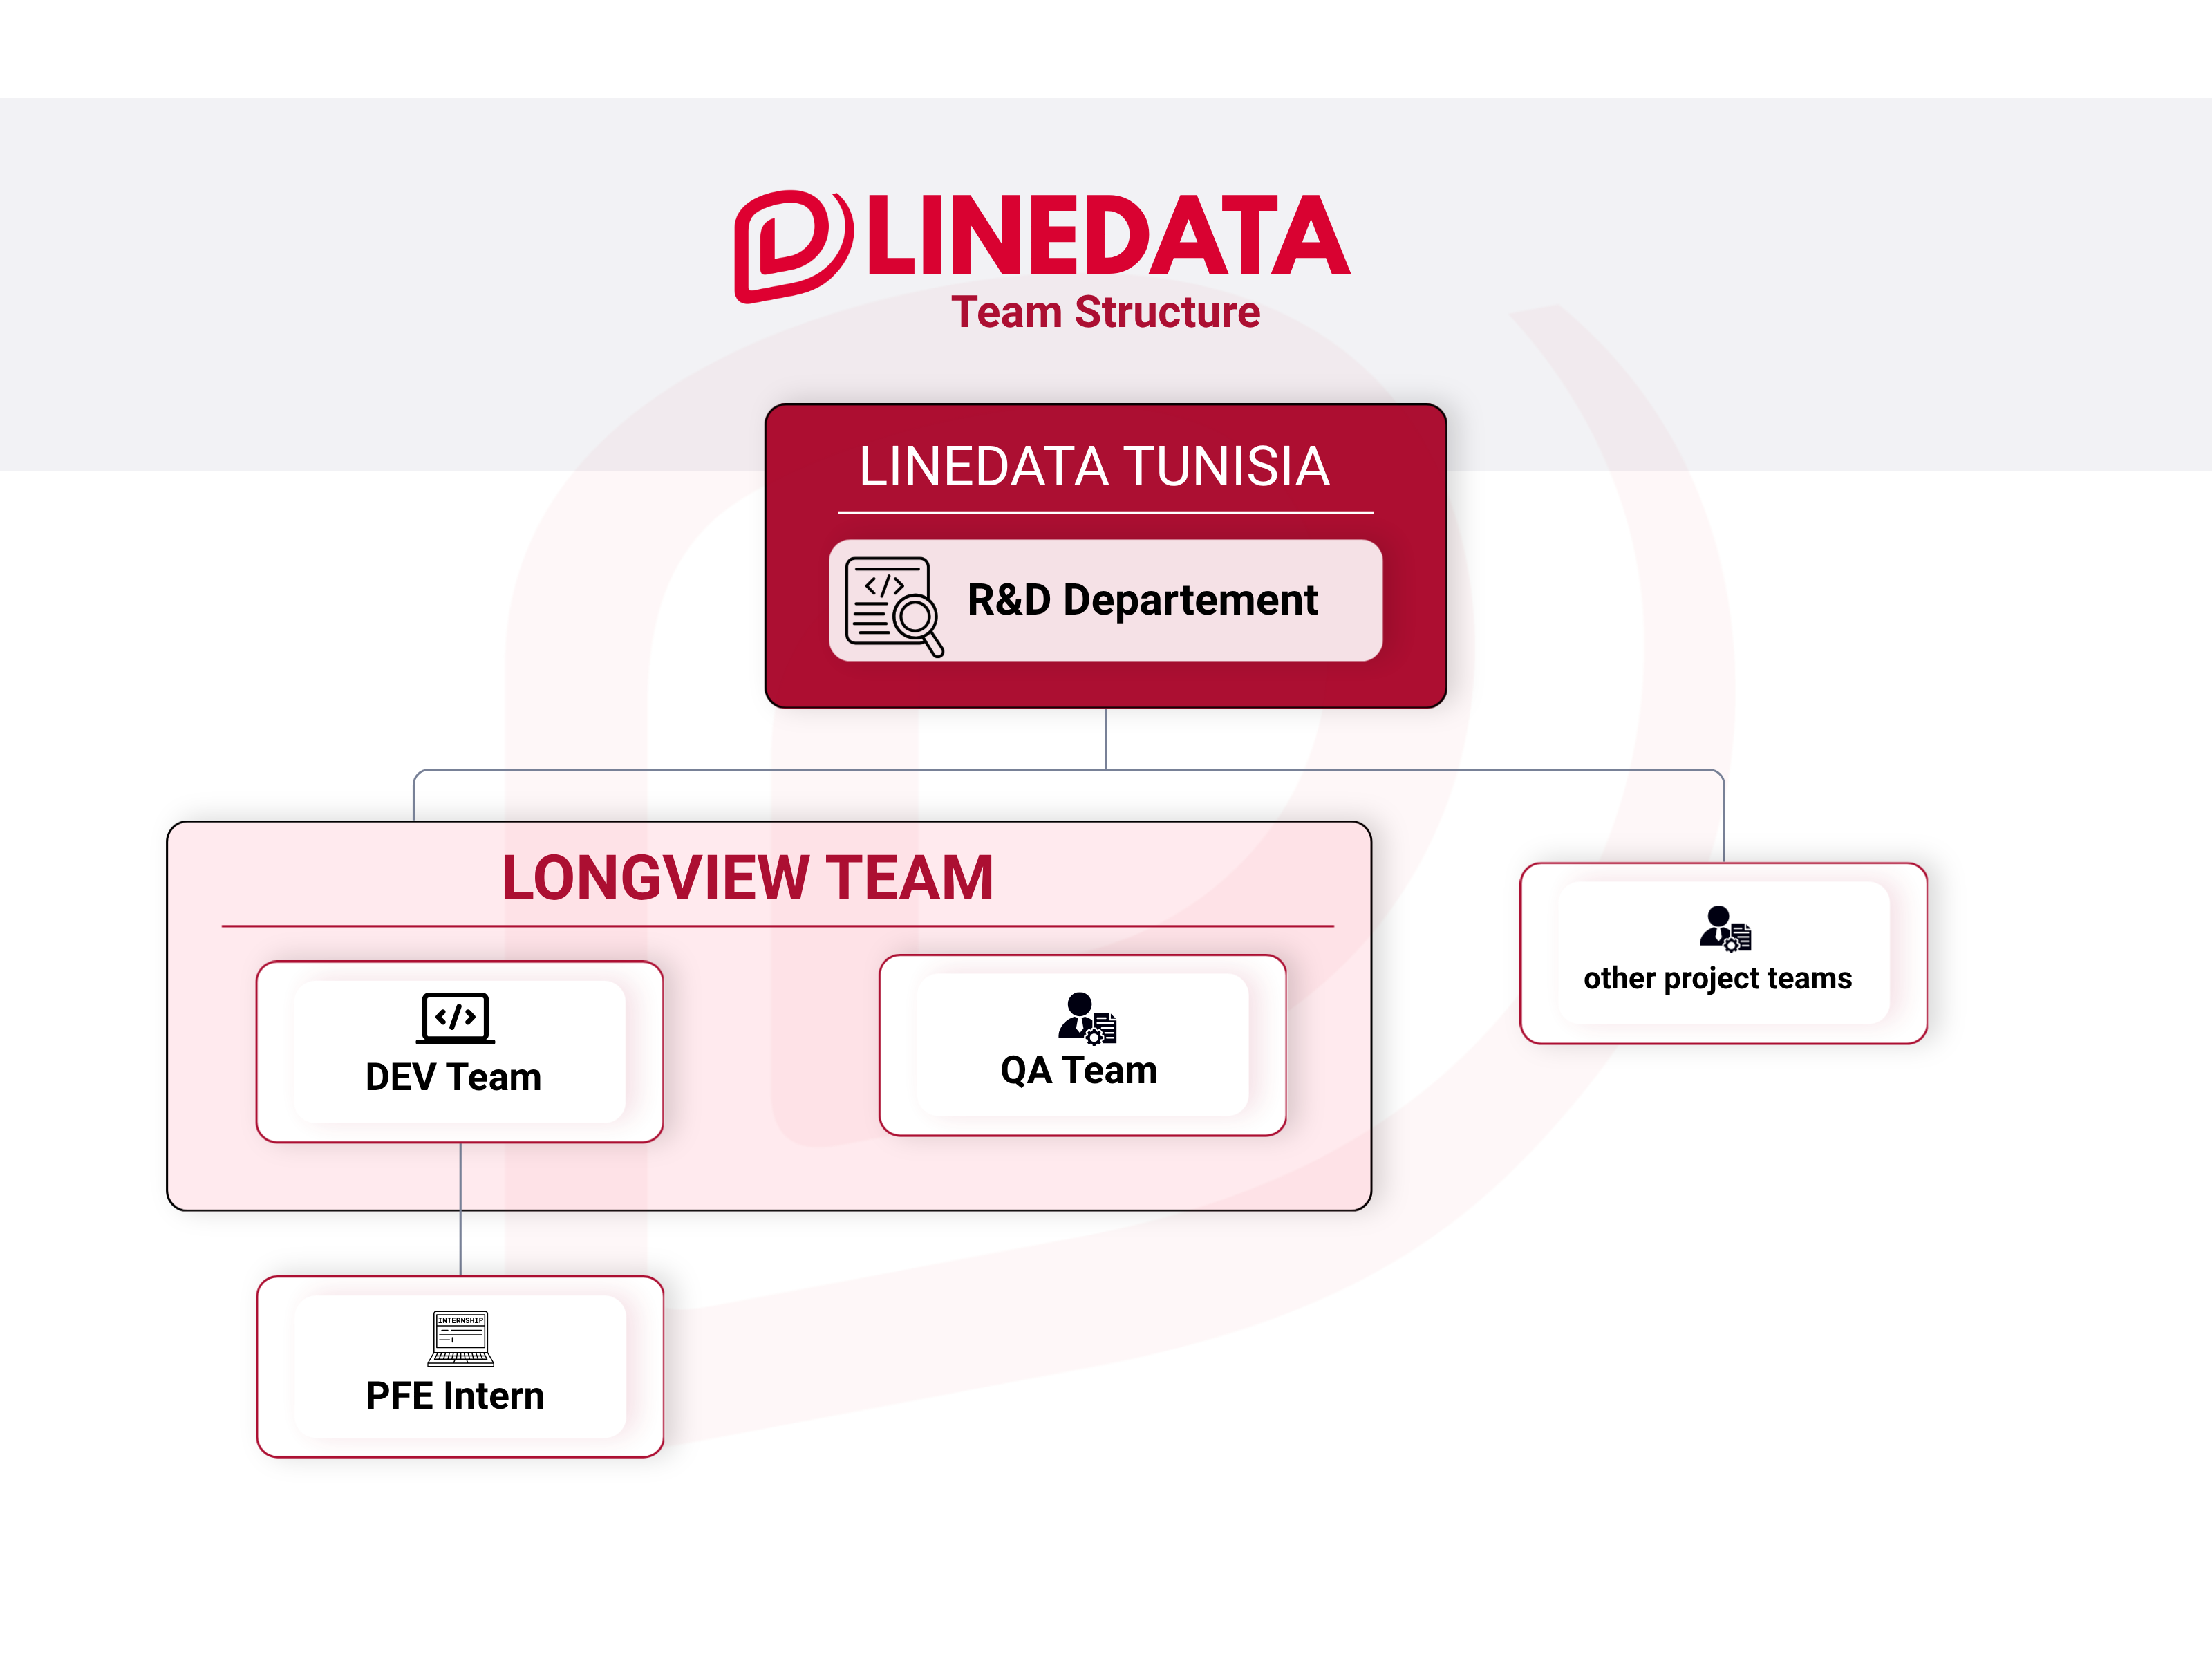
\includegraphics[width=0.82\textwidth]{img/orgchart.png}
\caption{Organizational structure of Linedata Tunisia and internship team placement}
\label{fig:orgchart}
\end{figure}

\paragraph{}The main goal of this internship was to design and build a configurable system that can generate valid test data for the Longview platform. This system was created to resolve the serious inefficiencies found in the existing manual test data preparation process.

% ─────────────────────────────────────────────
\section{Longview}
% ─────────────────────────────────────────────

\begin{figure}[htbp]
\centering
\includegraphics[width=0.5\textwidth]{img/longview_logo.png}
\caption{Linedata Longview, Front-Office Trade Order Management Platform \cite{longview_oms}}
\label{fig:longview}
\end{figure}

\paragraph{}Longview is an integrated, multi-tenant front-office trade order management platform built specifically for buy-side financial institutions. The platform supports the full investment lifecycle, including portfolio construction, compliance checks, order management, electronic trade execution, and post-trade settlement. Built on a relational SQL Server database, Longview supports continuous global trading operations and automated end-to-end processing. At the time of this project, the platform was at version 8.2 and continues to receive regular maintenance and improvements \cite{longview_oms}.

% ─────────────────────────────────────────────
\subsection{Core Financial Entities}
% ─────────────────────────────────────────────

\paragraph{}The Longview data model is built around a set of related financial entities that must maintain strict referential integrity and comply with business rule constraints. The platform's architecture is centered on several key entity types, including Accounts, Securities, Orders, Executions, and Positions.

\begin{itemize}
\item \textbf{Accounts:} Investment portfolios or client mandates, each identified by a unique account ID, linked to a base currency, a portfolio manager, and optional regulatory and compliance attributes.
\item \textbf{Securities:} Financial instruments across multiple asset classes, including equities and funds, fixed income instruments (bonds, money market securities, mortgage pass-throughs), futures, options, and FX forwards. Each type has its own required fields and valuation rules.
\item \textbf{Orders:} Buy or sell instructions created by portfolio managers, linked to specific accounts and securities, and subject to quantity, timing, and allocation constraints.
\item \textbf{Executions and Positions:} Trade confirmations produced when orders are filled, and the resulting inventory positions held by each account across its securities.
\end{itemize}

\paragraph{}The complex relationships and constraints between these entities make generating valid test data a challenging task. Any violation of referential integrity or business rules makes a dataset unusable and reduces the effectiveness of the quality assurance process.

% ─────────────────────────────────────────────
\section{Current Testing Procedure}
% ─────────────────────────────────────────────

\paragraph{}Ensuring the correctness and reliability of each Longview release requires a solid and continuous testing process. The quality assurance and development teams are responsible for validating new features, running regression tests, and confirming that existing functionality is preserved as the platform evolves. This process depends on having relevant, varied, and realistic test datasets.

% ─────────────────────────────────────────────
\subsection{Manual Test Data Preparation}
% ─────────────────────────────────────────────

\paragraph{}Currently, test data is generated through mostly manual procedures. Quality assurance engineers and developers write SQL scripts by hand and execute them against the Longview SQL Server database using INSERT, TRUNCATE, and IDENTITY\_INSERT statements, as well as stored procedure calls. For each test scenario, team members must identify the relevant database tables, manually build valid records that satisfy all primary and foreign key relationships, and verify that the data follows Longview's business rules. This process requires a thorough understanding of both the SQL Server schema and financial domain logic.

% ─────────────────────────────────────────────
\subsection{Limitations of the Current Approach}
% ─────────────────────────────────────────────

\paragraph{}The manual approach has several important limitations that reduce the efficiency, coverage, and reliability of the quality assurance process:

\begin{itemize}
\item \textbf{Time-consuming:} Building a complete dataset across multiple dependent tables can take hours for complex scenarios, such as full trade lifecycles involving group orders, multi-account allocations, and broker tickets.
\item \textbf{Error-prone:} Human mistakes such as mismatched foreign keys, execution quantities exceeding the parent order quantity, or missing price records frequently cause test failures that are unrelated to the feature being tested, leading to wasted debugging time.
\item \textbf{Lack of reproducibility:} Test data is created on an ad hoc basis and is not stored in a structured, version-controlled format, making it difficult to reproduce, share, or reuse across regression cycles.
\item \textbf{Confidentiality constraints:} Production data cannot be used for testing due to strict confidentiality agreements and regulatory requirements, so teams must rely entirely on artificially constructed datasets.
\end{itemize}

\begin{figure}[htbp]
\centering
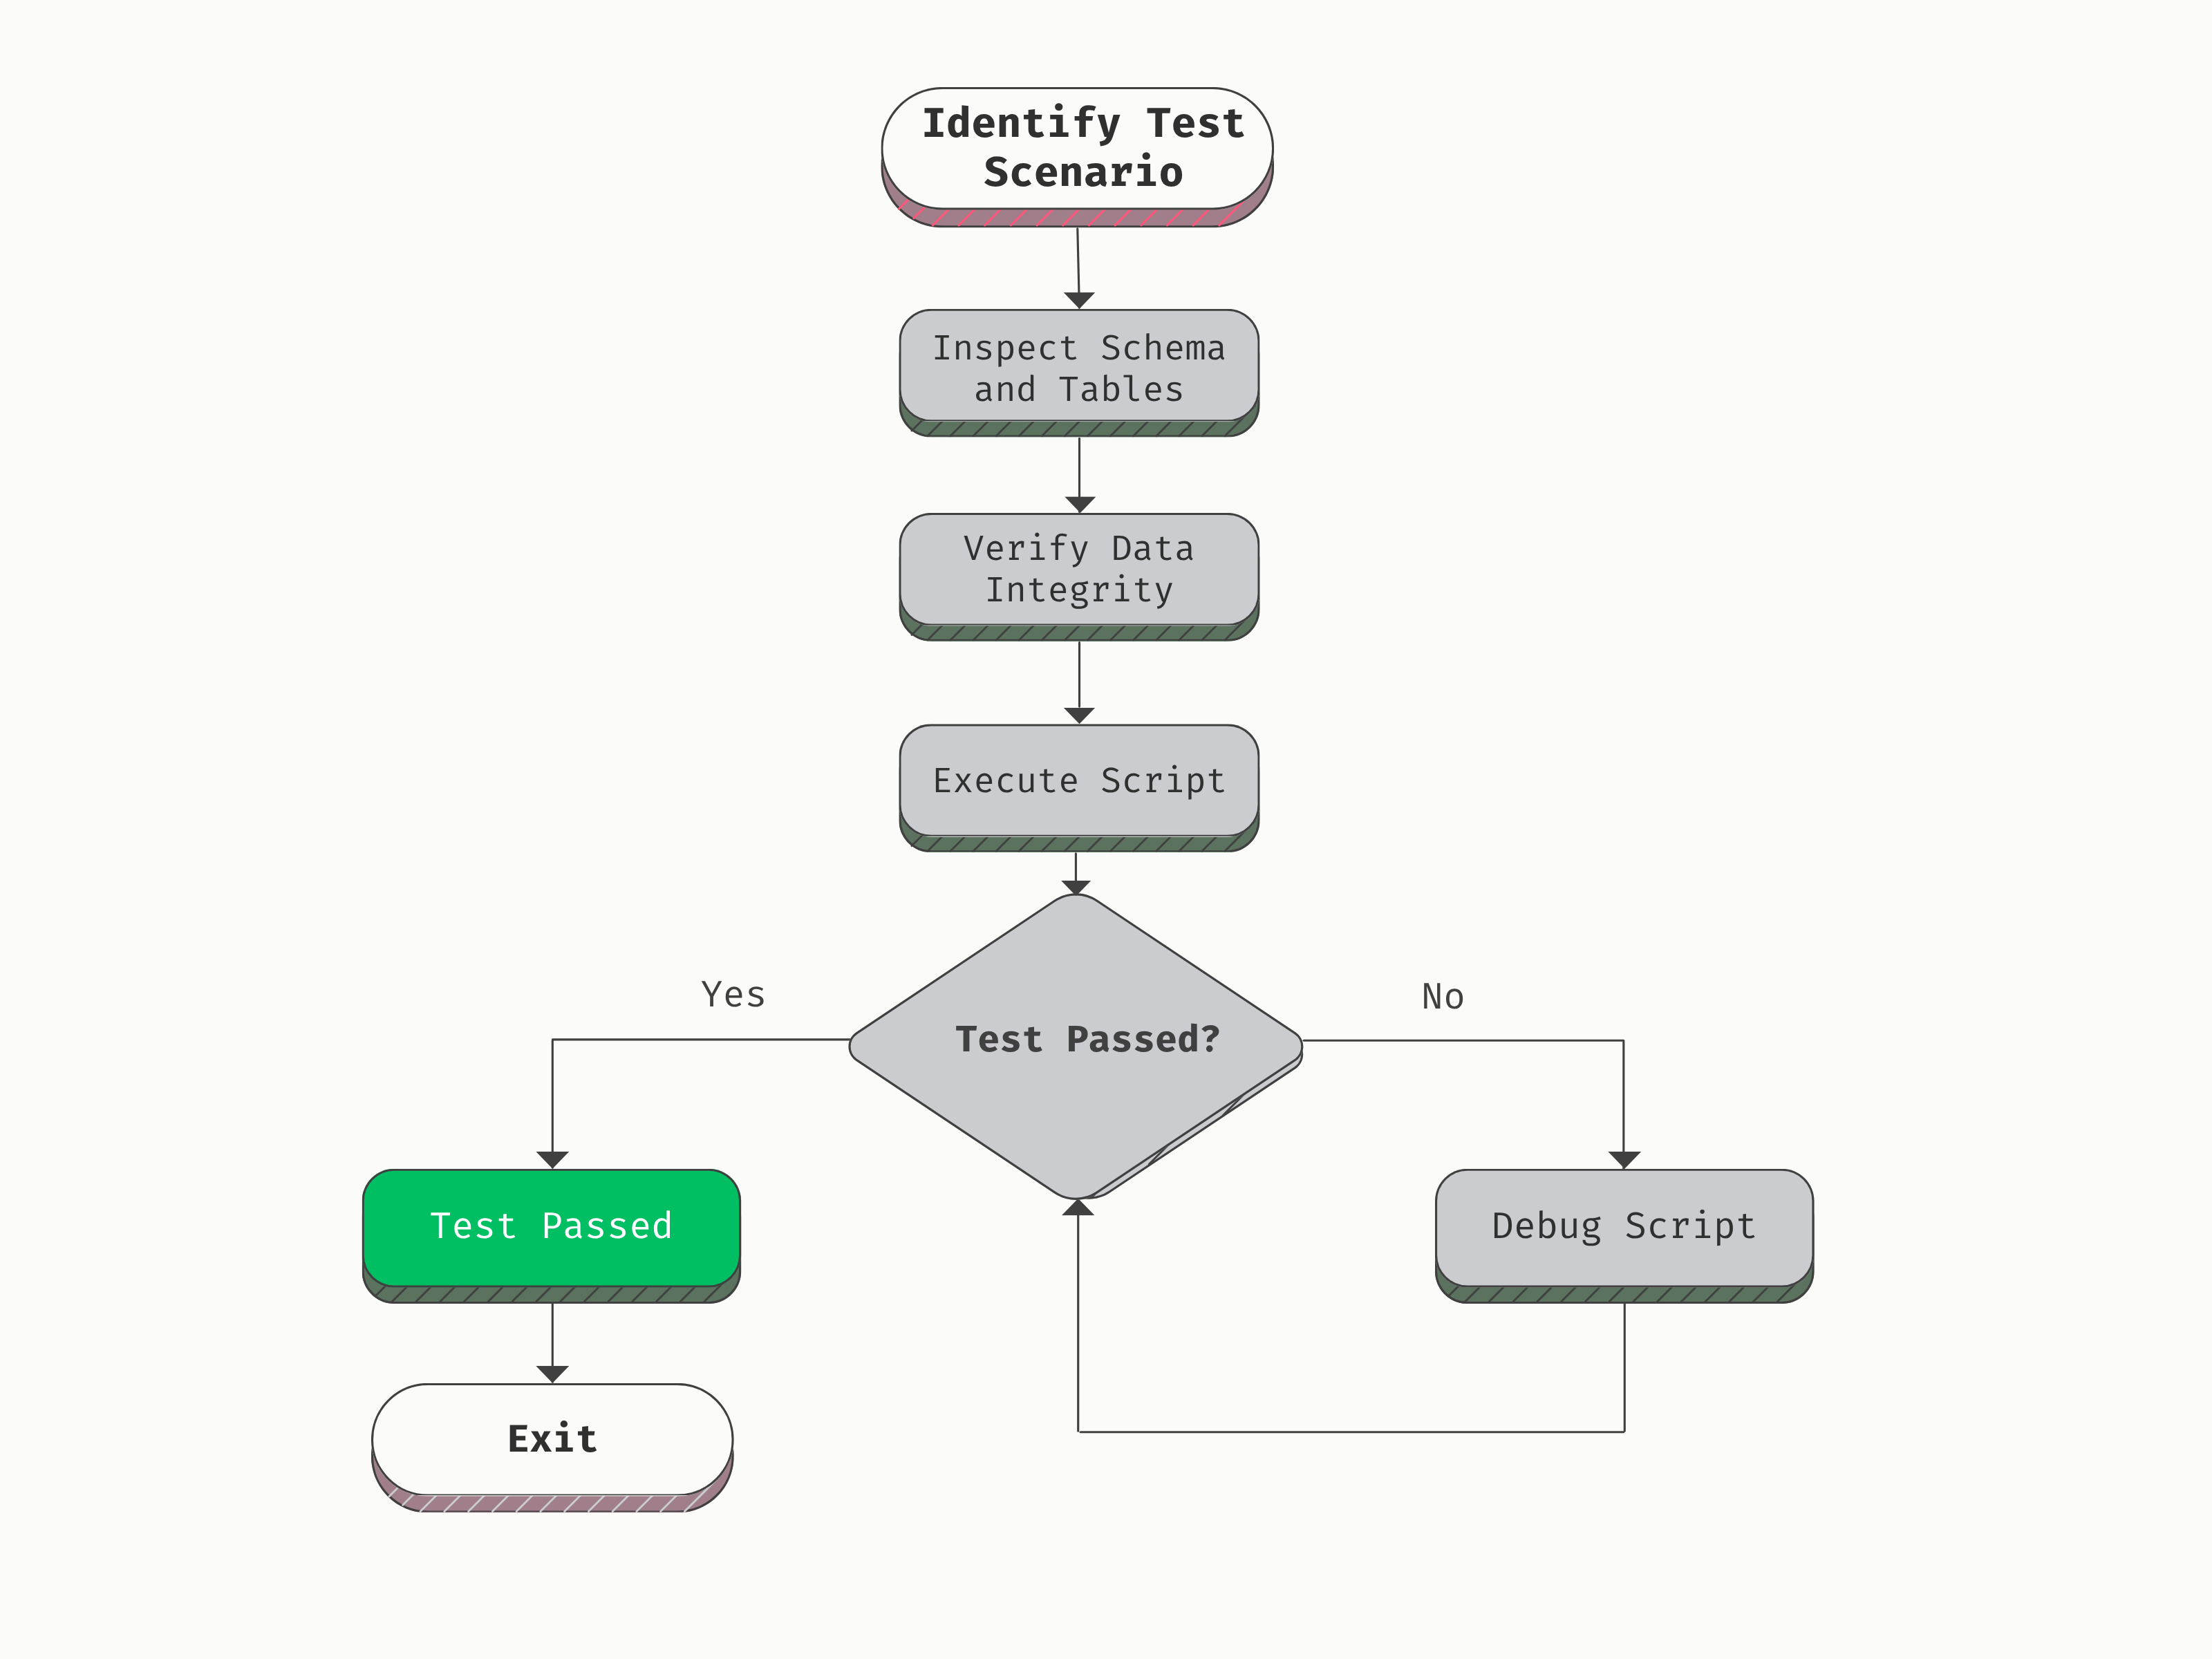
\includegraphics[width=0.85\textwidth]{img/current-process.png}
\caption{Current manual test data creation workflow at Linedata}
\label{fig:current-process}
\end{figure}

% ─────────────────────────────────────────────
\section{Problem Statement}
% ─────────────────────────────────────────────

\paragraph{}These limitations together point to a significant gap in Linedata's testing infrastructure. As the Longview platform expands to support a wider range of financial instrument types and regulatory frameworks, the need for varied and quickly deployable test data grows accordingly. The current manual approach is not able to meet these growing demands.

\paragraph{}This situation leads to the central problem statement of this project: \textit{How can Linedata's development and quality assurance teams be provided with an automated, configurable, and domain-aware tool that can generate realistic, coherent, and SQL-compatible test data for the Longview platform, while correctly enforcing the complex relationships between entities and the financial business rules that govern its data model?}

\paragraph{}This question breaks down into three core challenges:

\begin{itemize}
\item \textbf{Financial data consistency:} Generating valid test data requires enforcing business rules across dozens of interdependent tables at the same time. Any violation makes the dataset unusable.

\item \textbf{Dual-mode operation:} The tool must work in two distinct modes. In \textit{standalone mode}, it generates fully synthetic data without needing any database connection. In \textit{connected mode}, it establishes a read-only connection to an existing Longview SQL Server instance, retrieves real reference data (securities, accounts, models), and generates additional records that are consistent with the existing database state.

\item \textbf{Configurability and usability:} Test engineers must be able to specify data volume, instrument types, date ranges, and other parameters through an easy-to-use web interface, save and reuse generation configurations through a local library, and access the tool without requiring deep technical knowledge.
\end{itemize}

\paragraph{}Addressing these challenges required designing and building a full-stack web application that includes modular generation services for each financial entity, read-only SQL Server integration for connected operation, a local configuration library for saving and reusing generation presets, and optional Large Language Model integration for improved data realism. The system remains fully functional even when LLM support is unavailable. This is the core system described and developed throughout the rest of this report.

% ─────────────────────────────────────────────
\section{Proposed Solution}
% ─────────────────────────────────────────────

\paragraph{}To address the identified challenges, a configurable test data generation system named \textbf{Longview Test Data Generator} has been designed and implemented. The system operates in two complementary modes: \textit{standalone mode} generates fully synthetic test data without requiring any database connection, while \textit{connected mode} integrates with an existing Longview SQL Server instance in read-only mode to retrieve reference data and generate supplementary records that remain consistent with the production environment. The application also includes a configuration library that allows users to save, reload, and reuse generation settings across testing sessions. Through these features, the tool provides QA engineers and developers with a flexible, automated approach to generating valid, realistic, and reproducible test datasets on demand.

% ─────────────────────────────────────────────
\section*{Conclusion}
\addcontentsline{toc}{section}{Conclusion}
% ─────────────────────────────────────────────

\paragraph{}This chapter has established the professional and technical context for this project. We introduced Linedata and its Tunisian office as the host organization, and identified the Longview development team as the internship setting. We presented the Longview platform and described the core financial entities that make up its data model. The chapter reviewed the current manual test data creation process and identified its main weaknesses in terms of efficiency, error management, and time consumption. Finally, we defined the central problem statement: the need for an automated, domain-aware, and configurable test data generation system for Longview that supports both standalone and connected operation modes. The following chapter presents the requirements analysis, the adopted development methodology, the global architecture, and the sprint planning of the project.

        \clearpage
        
        % !TeX root = main.tex

\chapter{Requirements Analysis and Global Design}


% ─────────────────────────────────────────────
\section*{Introduction}
\addcontentsline{toc}{section}{Introduction}
% ─────────────────────────────────────────────

\paragraph{}With the project context and problem statement established in
the previous chapter, this chapter moves into the analysis and design phase.
We begin by presenting the Agile Scrum methodology adopted to structure the
work across the internship period. We then examine existing tools that
address similar problems and explain why none of them were suitable for this
specific context. From there, we derive the functional and non-functional
requirements the system must satisfy, translate them into a global
architecture, and present the product backlog and sprint plan that guided
the implementation. The chapter closes with a description of the technical
environment used throughout the project.


% ─────────────────────────────────────────────
\section{Development Methodology}
% ─────────────────────────────────────────────

\paragraph{}Since the QA team are the primary users of this application, their feedback was essential at every stage of the development process, so they could review the delivered features and provide concrete feedback on what needed to be improved, removed, or added. This close and continuous collaboration made Agile the best choice, as it is built around short delivery cycles that end with a review, allowing the product to be shaped progressively based on real user input. Among the available Agile frameworks, Scrum was selected for its simple structure, its defined feedback points at the end of each sprint, and its ability to incorporate changes without disrupting the overall plan \cite{schwaber2020scrum}.


% ─────────────────────────────────────────────
\subsection{Scrum Framework Overview}
% ─────────────────────────────────────────────

\paragraph{}Scrum organizes work into fixed-length iterations called
\textbf{sprints}, each ending with a potentially shippable increment of the
product. Three core roles structure the team, three artifacts capture the
work, and four ceremonies punctuate each sprint cycle, as illustrated in
Figure~\ref{fig:scrum}.

\begin{figure}[H]
\centering
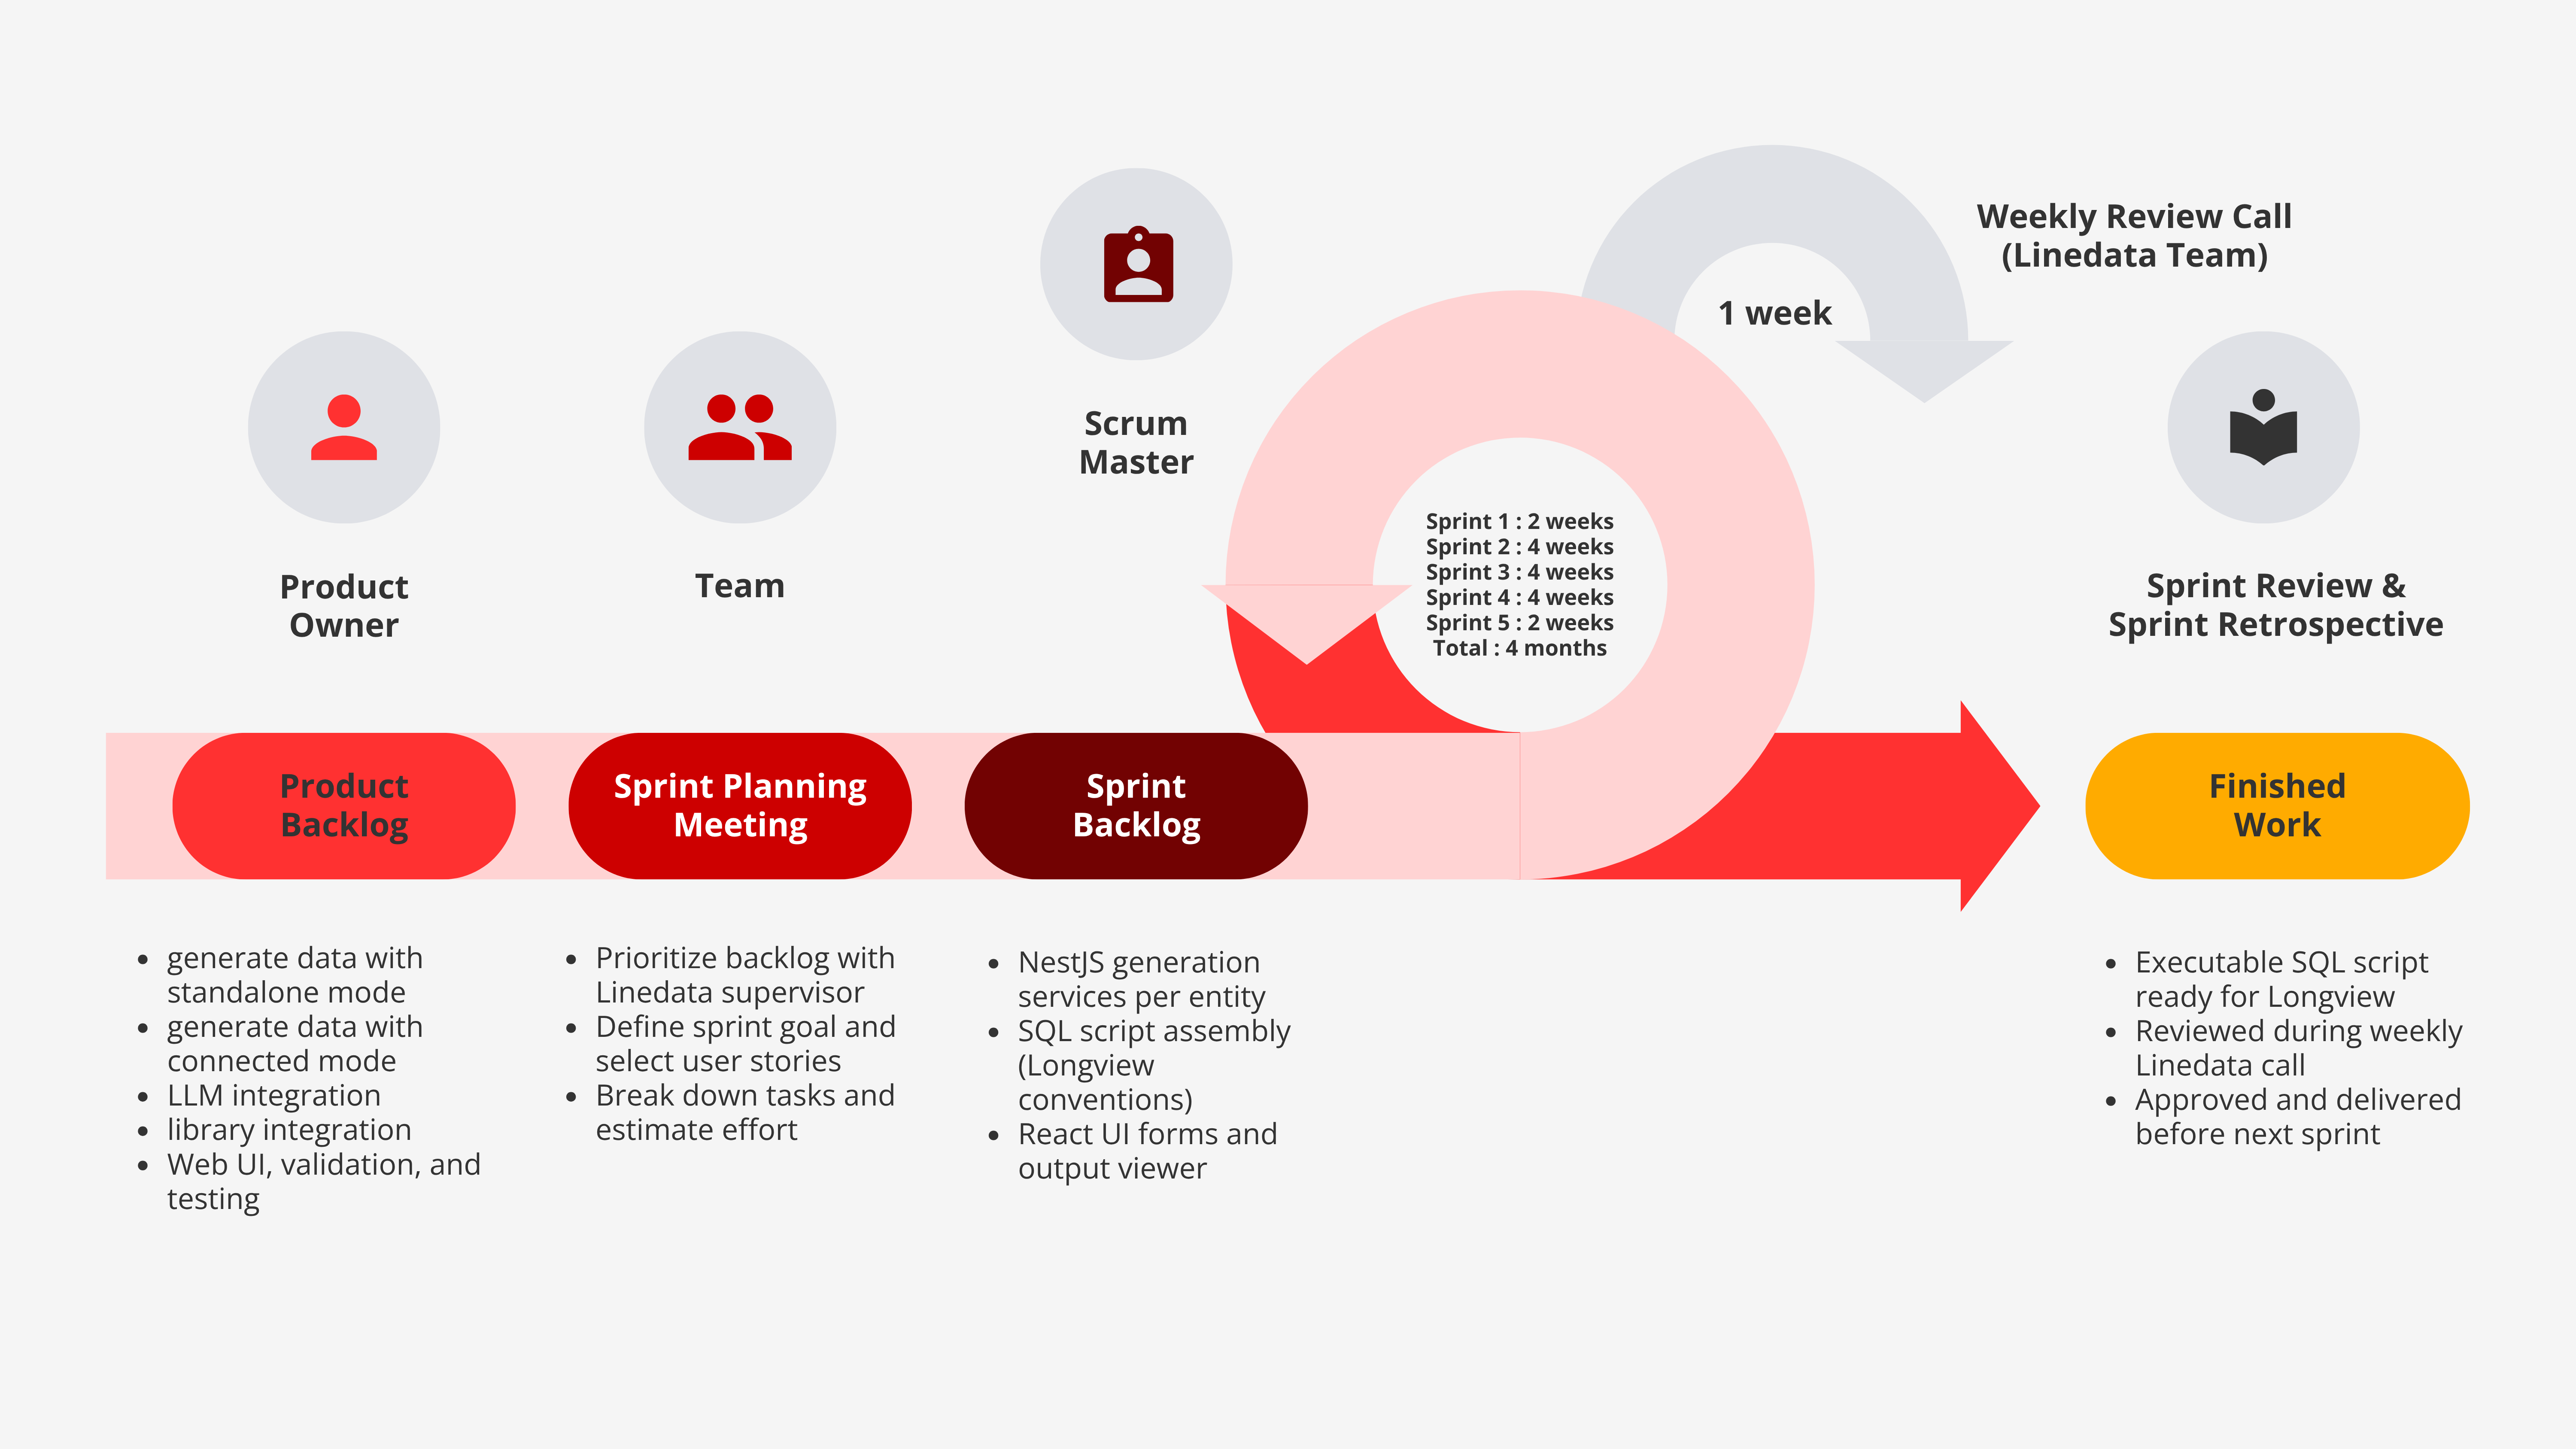
\includegraphics[width=0.85\textwidth]{img/scrum-process.png}
\caption{The Scrum process framework}\label{fig:scrum}
\end{figure}

\paragraph{}Within this project, the Scrum roles were adapted to the
internship context as follows:

\begin{itemize}
    \item \textbf{Product Owner:} The internship supervisor at Linedata,
    responsible for defining priorities, validating deliverables, and
    ensuring the tool aligned with the team's actual testing needs.
    \item \textbf{Scrum Master / Developer:} The intern, responsible for
    planning, executing, and delivering each sprint increment, managing
    impediments, and adjusting scope when needed.
\end{itemize}

\paragraph{}The Scrum artifacts and ceremonies were applied as follows:

\begin{itemize}
    \item \textbf{Product Backlog:} A prioritized list of all features and
    tasks to be delivered across the project lifetime.
    \item \textbf{Sprint Backlog:} The subset of backlog items committed to
    for each sprint, refined at the start of each cycle.
    \item \textbf{Sprint Increment:} The functional, testable deliverable
    produced at the end of each sprint, demonstrated to the supervisor
    during the sprint review.
    \item \textbf{Weekly Review Call:} Given the internship context,
    the classical daily stand-up was replaced by a weekly call with
    the Linedata development team, during which progress was demonstrated,
    feedback was collected, and priorities for the coming week were adjusted.
\end{itemize}


% ─────────────────────────────────────────────
\subsection{Sprint Planning Overview}
% ─────────────────────────────────────────────

\paragraph{}The internship was organized into five sprints, each targeting
a distinct phase of the project. Figure~\ref{fig:sprint-plan} gives an
overview of the sprint plan.

\begin{figure}[H]
\centering
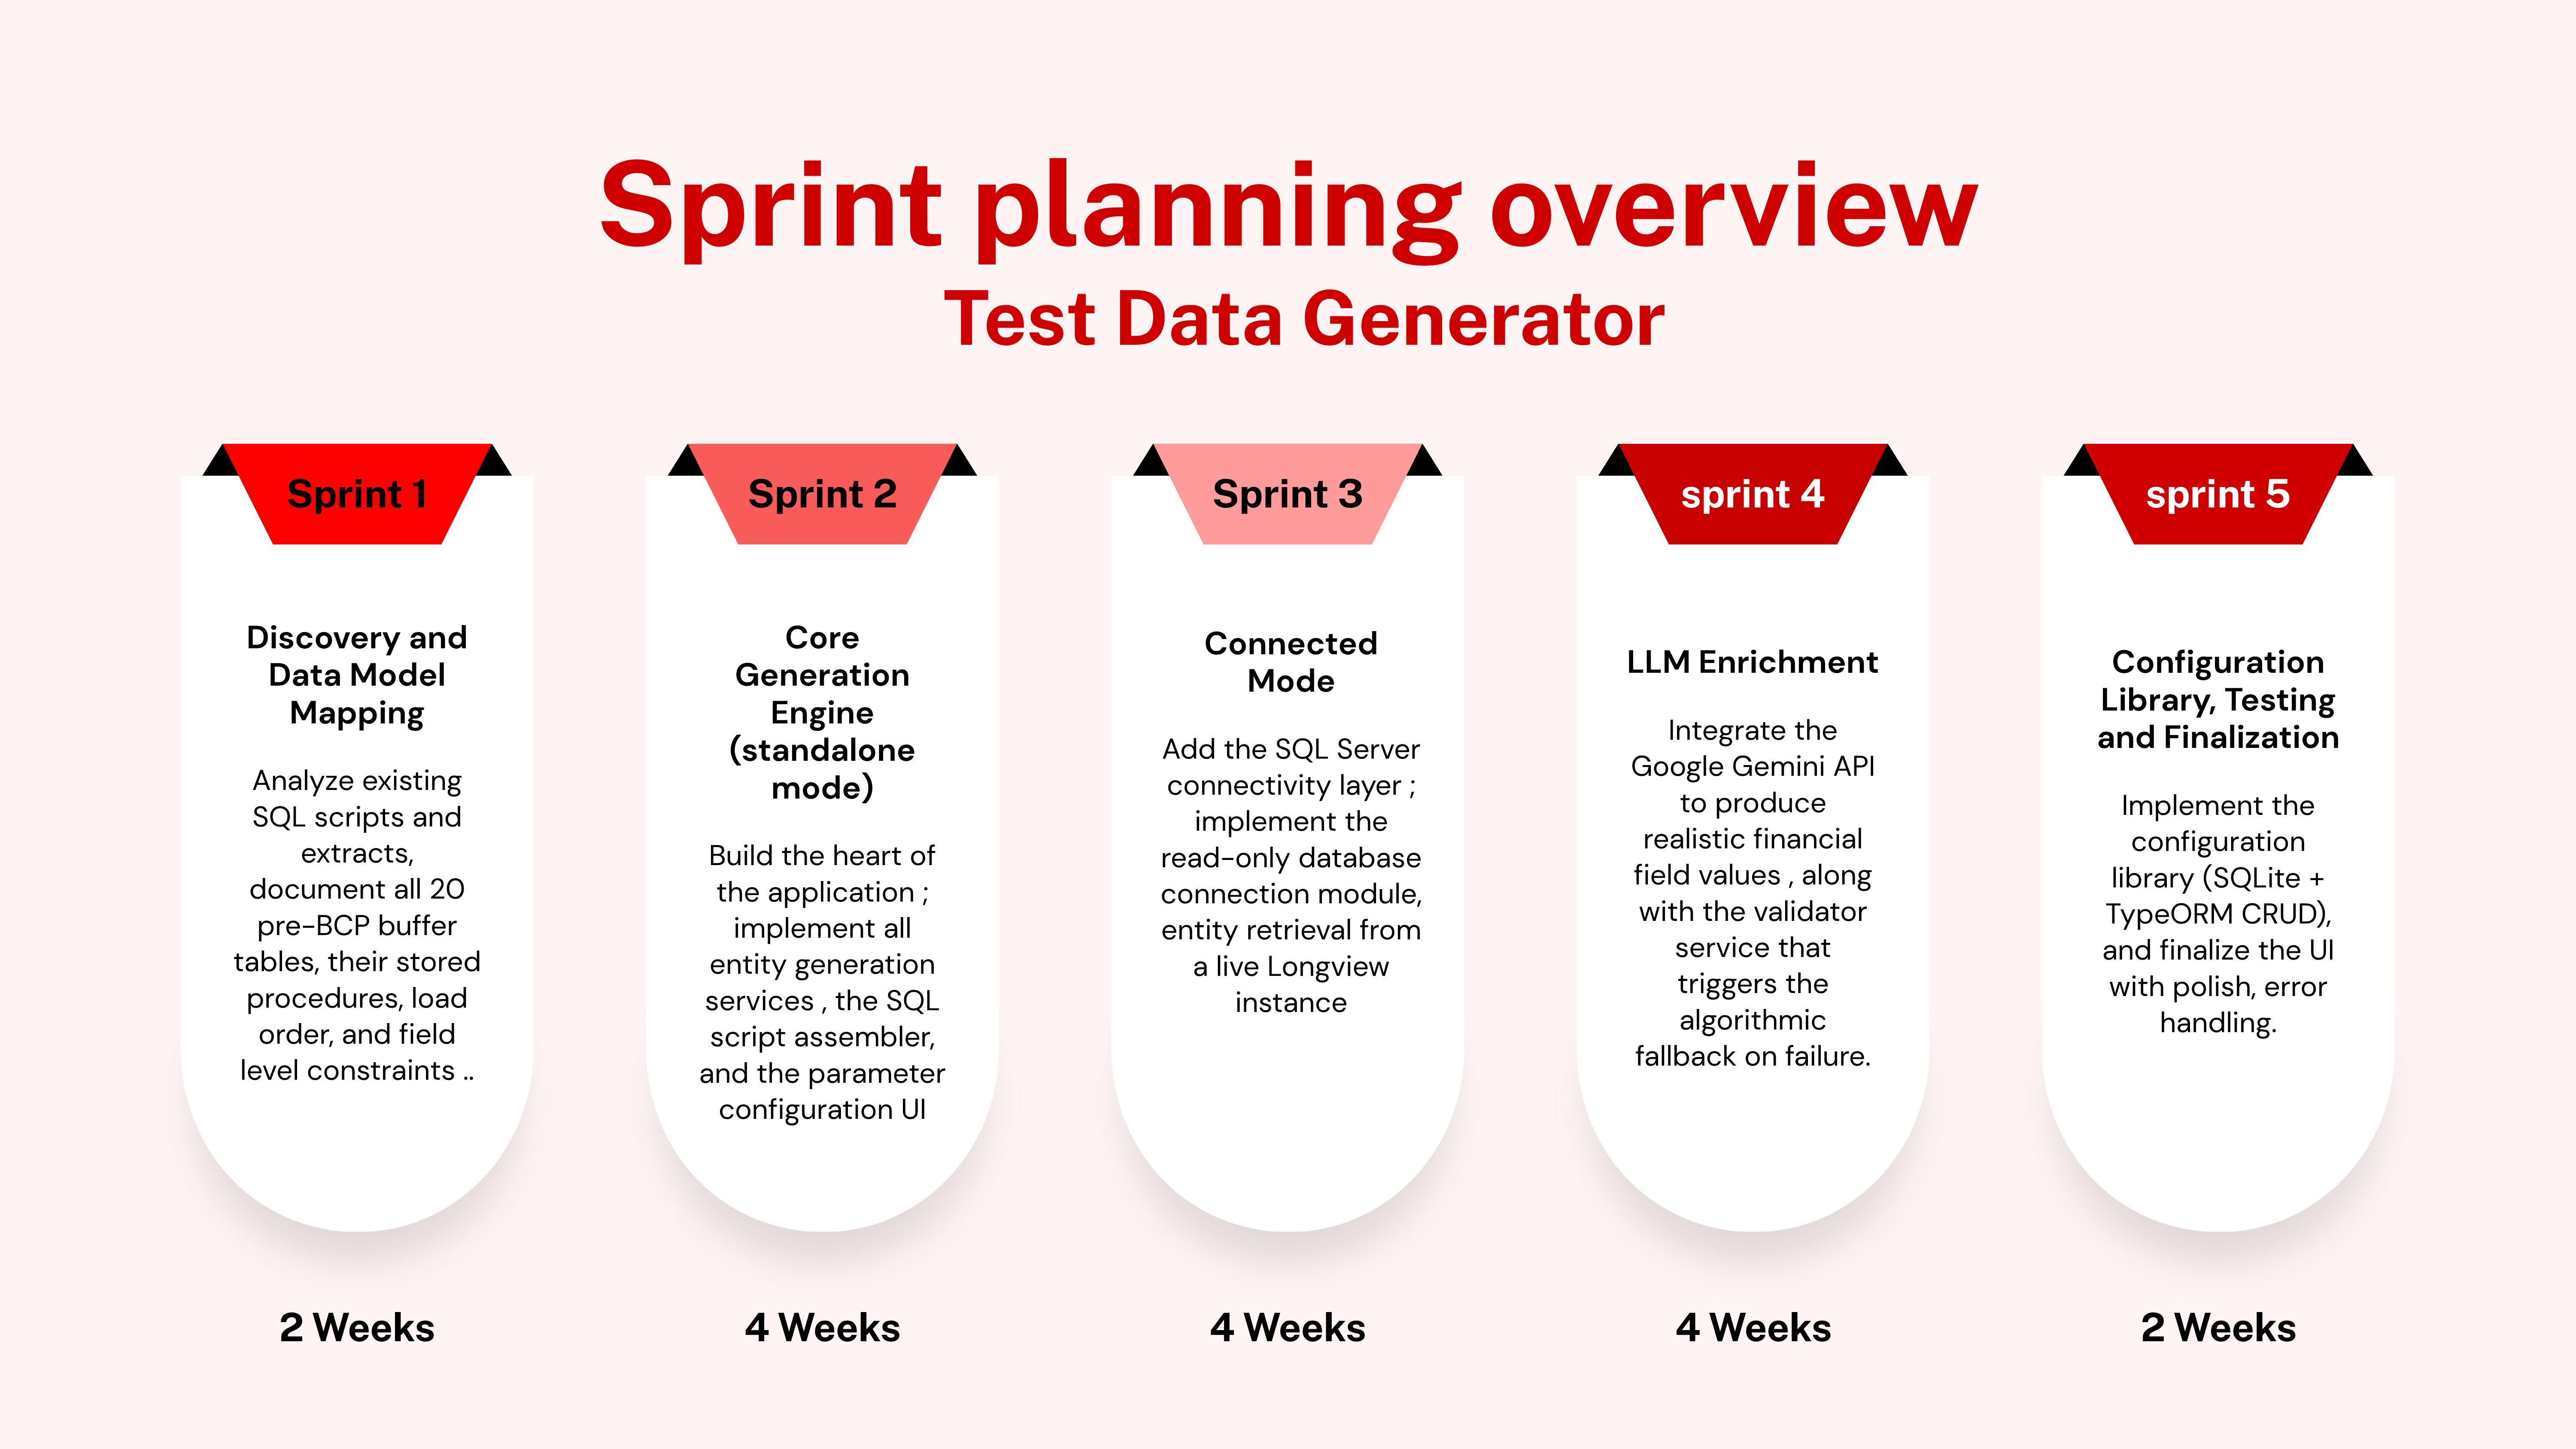
\includegraphics[width=0.95\textwidth]{img/sprint-plan.png}
\caption{Sprint planning overview}
\label{fig:sprint-plan}
\end{figure}


% ─────────────────────────────────────────────
\section{Study of Existing Solutions}
% ─────────────────────────────────────────────

\paragraph{}Before designing anything, we examined the tools and approaches
that already exist in the space of test data generation. Understanding where
they fall short in this specific context helps justify the decision to build
a custom solution.


% ─────────────────────────────────────────────
\subsection{Generic Test Data Generation Tools}
% ─────────────────────────────────────────────

\paragraph{}The most commonly used tools for generating synthetic test data
fall into three categories:

\begin{itemize}
    \item \textbf{Mockaroo} \cite{mockaroo}: A web-based tool that generates
    random data across a wide range of field types and exports it in various
    formats including SQL, CSV, and JSON. It is quick to use for simple flat
    datasets but has no concept of relational integrity or cross-table
    dependencies.

    \item \textbf{Faker} \cite{faker}: A widely
    used library available in Python, JavaScript, and other languages that
    generates plausible fake data (names, addresses, numbers, and dates).
    It is effective for populating individual fields with realistic-looking
    values, but it operates at the field level, not the dataset level.

    \item \textbf{Redgate SQL Data Generator} \cite{redgate}: This tool is
    closer to the target use case, it generates SQL \texttt{INSERT}
    statements for relational schemas and can respect foreign key
    relationships. However, it operates on a generic schema inference basis.
    It has no knowledge of financial domain rules, no concept of Longview's
    pre-BCP buffer mechanism, and no way to produce the specific Unicode
    casting and type conventions the platform requires.
\end{itemize}


% ─────────────────────────────────────────────
\subsection{Comparison Summary}
% ─────────────────────────────────────────────

\paragraph{}Table~\ref{tab:tools-comparison} summarizes how each existing
solution covers the key requirements of this project.

\begingroup
\setlength{\tabcolsep}{5pt}
\renewcommand{\arraystretch}{1.25}
\newcommand{\yes}{\textcolor{green!45!black}{\cmark}}
\newcommand{\no}{\textcolor{red!70!black}{\xmark}}
\arrayrulecolor{isiBlue!45}
\begin{longtable}{P{0.34\textwidth}
                Q{0.12\textwidth}
                Q{0.12\textwidth}
                Q{0.12\textwidth}
                Q{0.14\textwidth}}
\caption{Comparison of existing tools against project requirements}
\label{tab:tools-comparison} \\
\hline
\rowcolor{isiBlue!15}
\textbf{Criterion}
  & \textbf{Mockaroo}
  & \textbf{Faker}
  & \textbf{Redgate}
  & \textbf{Our Solution} \\
\hline
\endfirsthead
\multicolumn{5}{r}{\tablename\ \thetable{} -- \textit{continued from previous page}} \\
\hline
\rowcolor{isiBlue!15}
\textbf{Criterion}
  & \textbf{Mockaroo}
  & \textbf{Faker}
  & \textbf{Redgate}
  & \textbf{Our Solution} \\
\hline
\endhead
\hline
\multicolumn{5}{r}{\textit{continued on next page}} \\
\endfoot
\hline
\endlastfoot
\rowcolor{gray!5} Relational integrity       & \no & \no & \yes & \yes \\
Financial business rules                      & \no & \no & \no  & \yes \\
\rowcolor{gray!5} Longview SQL conventions    & \no & \no & \no  & \yes \\
LLM-enriched realism                          & \no & \no & \no  & \yes \\
\rowcolor{gray!5} Connected mode (read-only)  & \no & \no & \no  & \yes \\
No manual post-processing                     & \no & \no & \no  & \yes \\
\rowcolor{gray!5} Configuration persistence   & \no & \no & \no  & \yes \\
\hline
\end{longtable}
\arrayrulecolor{black}
\endgroup

\paragraph{}The gap these tools all share comes down to the same root cause:
they are built for the general case, not for a specific financial platform
with its own data model, its own loading conventions, and its own business
rules. This analysis confirmed that a purpose-built solution was the right
path, and that the core value of the tool lies precisely in the domain
knowledge encoded into its generation logic.


% ─────────────────────────────────────────────
\section{Requirements}
% ─────────────────────────────────────────────

% ─────────────────────────────────────────────
\subsection{Functional Requirements}
% ─────────────────────────────────────────────

\paragraph{}The functional requirements were gathered through analysis of
the existing Extracts, discussions with the Longview development and QA team,
and review of the project brief. They are organized around the two operating
modes of the system, followed by the LLM enrichment that applies to both.
The following table presents the identified functional requirements
organized by actor.

\begin{longtable}{|P{3cm}|P{10cm}|}
\caption{Description of functional requirements by actor}
\label{tab:functional-requirements} \\
\hline
\textbf{Actor} & \textbf{Functional Requirements} \\
\hline
\endfirsthead

\multicolumn{2}{r}{\tablename\ \thetable{} -- \textit{continued from previous page}} \\
\hline
\textbf{Actor} & \textbf{Functional Requirements} \\
\hline
\endhead

\hline
\multicolumn{2}{r}{\textit{continued on next page}} \\
\endfoot

\hline
\endlastfoot

QA Engineer
  & \begin{itemize}[noitemsep, topsep=2pt, leftmargin=*]
      \item Configure generation parameters (accounts, securities,
            orders, executions, positions, date ranges, asset classes)
            through a web interface
      \item Generate a complete, executable SQL script in standalone mode
            without any database connection
      \item Provide SQL Server credentials and test connectivity in
            connected mode
      \item Browse and select existing database entities (accounts,
            securities, models) to anchor generated records
      \item Trigger LLM-enriched generation for improved data realism
      \item Download the generated SQL script from the web interface
      \item Save the current generation configuration to the local
            library with a name and optional description
      \item Browse, load, rename, and delete previously saved
            configurations from the library
    \end{itemize} \\
\hline
Longview SQL Server
  & \begin{itemize}[noitemsep, topsep=2pt, leftmargin=*]
      \item Expose existing account groups, accounts, and securities
            to the system in read-only mode (connected mode only)
    \end{itemize} \\
\hline
Google Gemini API
  & \begin{itemize}[noitemsep, topsep=2pt, leftmargin=*]
      \item Receive structured prompts and return realistic financial
            field values (security names, symbols, descriptions)
      \item Trigger the algorithmic fallback transparently on
            unavailability or invalid response
    \end{itemize} \\
\hline
Local SQLite Database
  & \begin{itemize}[noitemsep, topsep=2pt, leftmargin=*]
      \item Persist named generation configurations (name,
            description, operating mode, and parameter JSON)
            across sessions in read-write mode
      \item Expose stored configurations to the backend for
            retrieval, update, and deletion via TypeORM
    \end{itemize} \\
\hline
\end{longtable}


\subsubsection{Global Use Case Diagram}

\paragraph{}Figure~\ref{fig:usecase-global} presents the global use case
diagram of the system. It summarizes the three main functional areas exposed
to the QA team: standalone generation, connected generation, and saved
configuration management. It also shows the external systems involved in the
generation process, namely the LLM API and the Longview SQL Server instance.

\begin{figure}[H]
\centering
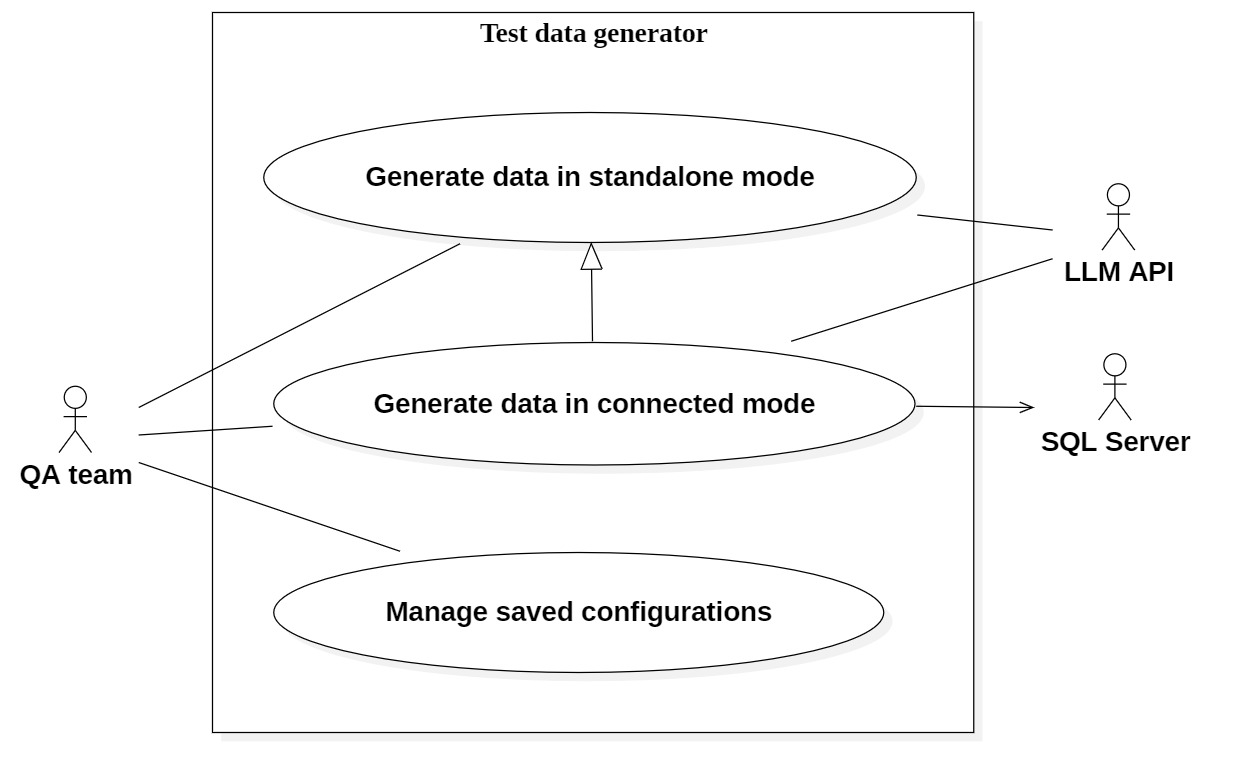
\includegraphics[width=0.9\textwidth]{img/usecase-global.jpg}
\caption{Global use case diagram of the test data generator}
\label{fig:usecase-global}
\end{figure}


% ─────────────────────────────────────────────
\subsection{Non-Functional Requirements}
% ─────────────────────────────────────────────

\paragraph{}Beyond what the system must do, the following quality
constraints shape how it must behave:

\begin{itemize}
    \item \textbf{Performance:} Generating a typical dataset -- one account
    with a full set of securities, orders, executions, and positions -- must
    complete within ten seconds in standalone mode for a typical QA dataset. LLM-assisted generation
    may take longer due to the network round-trip, but the experience must
    remain responsive from the user's perspective.

    \item \textbf{Resilience:} The system must remain fully operational
    regardless of LLM availability. If the Gemini API is unreachable or
    returns an invalid response, the algorithmic fallback must engage silently
    and complete the generation without user intervention.

    \item \textbf{Security:} The connected mode must operate in strict
    read-only mode. The application must have no capability to write, update,
    or delete data in any connected database. Connection credentials must not
    be persisted or logged beyond the active session.

    \item \textbf{Validation:} Generated datasets must be validated before
    delivery. The validator must check required fields, value formats,
    referential integrity, order and execution quantity consistency, and
    position derivation rules so that invalid records are detected before
    they reach the QA database.

    \item \textbf{Reproducibility:} A generation configuration must be
    saveable and reloadable so the same scenario can be repeated during
    regression testing. The generated output must be structured and
    inspectable, making it possible for QA engineers to archive and replay
    important scenarios.

    \item \textbf{Maintainability:} The generation logic for each entity type
    must be isolated in its own service module, so that updating a business
    rule or adding a new instrument type does not require changes across the
    entire codebase.

    \item \textbf{Extensibility:} The architecture must make it
    straightforward to add new entity types, asset classes, or output formats
    in the future without restructuring the core engine.

    \item \textbf{Usability:} The web interface must be accessible to QA
    engineers who are not necessarily developers. Error messages must be
    explicit, form inputs must be validated before submission, the generated
    SQL output must be easy to download, and frequently used parameter sets
    must be saveable and reloadable without manual re-entry.

    \item \textbf{Data Persistence:} Saved configurations must survive
    application restarts. The local SQLite database must be created
    automatically on first launch without requiring any manual installation
    or configuration from the user.
\end{itemize}


% ─────────────────────────────────────────────
\section{Global Architecture}
% ─────────────────────────────────────────────

\paragraph{}The requirements above point toward a full-stack web application
with a clear separation between the user interface, the generation logic, the
LLM integration, the database access layer, and the local configuration
persistence layer. The global package diagram is used as the logical/module
view of the solution, while the physical architecture diagram focuses on where
the main runtime elements are deployed and how they communicate.


% ─────────────────────────────────────────────
\subsection{Global Package Diagram}

\paragraph{}Figure~\ref{fig:global-package-diagram} presents the global package diagram of the application.
It serves as the logical organization view of the system. It shows how the frontend modes,
backend API, generation services, configuration library, LLM enrichment layer, and database
access services are organized and how they collaborate around the generated dataset and saved
configurations.

\begin{figure}[H]
\centering
\makebox[\textwidth][c]{%
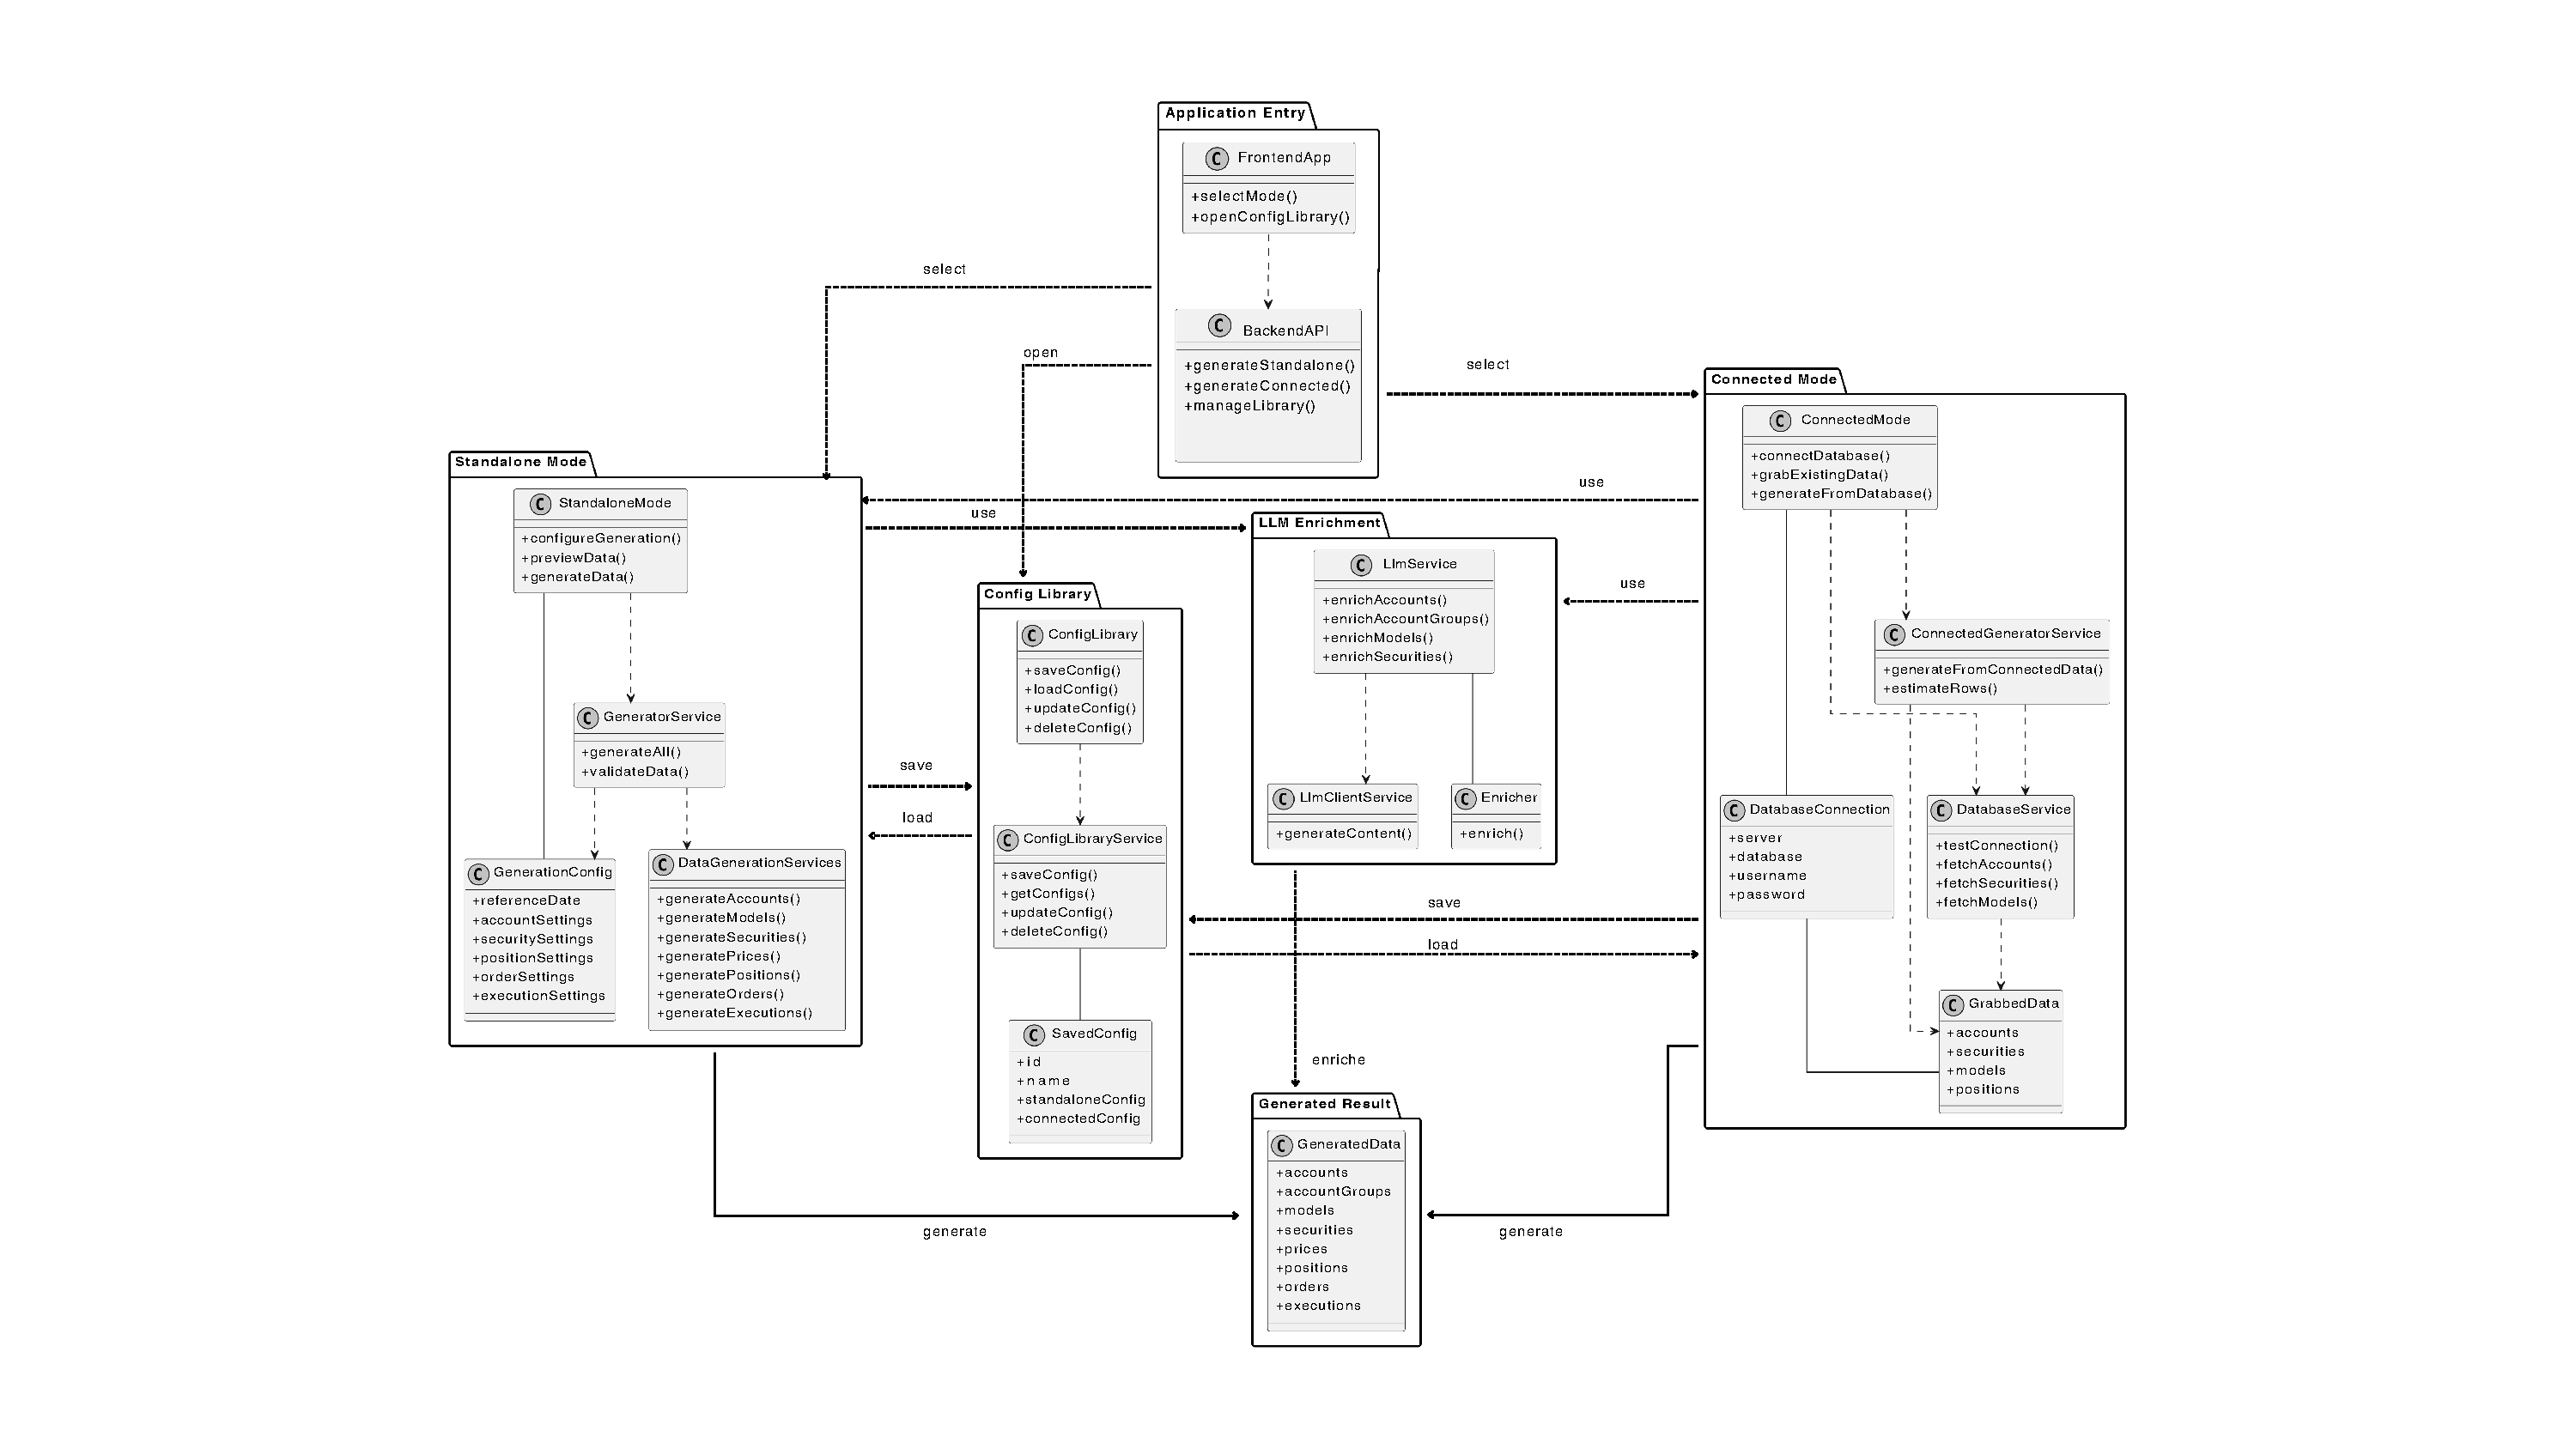
\includegraphics[width=1.4\textwidth,height=0.92\textheight,keepaspectratio]{img/global-package-diagram.pdf}}
\caption{Global package diagram of the test data generator}
\label{fig:global-package-diagram}
\end{figure}


% ─────────────────────────────────────────────

% ─────────────────────────────────────────────
\subsection{Physical Architecture}
% ─────────────────────────────────────────────

\paragraph{}Figure~\ref{fig:arch-physical} presents the physical architecture of the
application. Unlike the package diagram, which explains the internal software
organization, this view shows the deployed runtime elements and the external
systems used by the application.

\begin{itemize}
    \item The \textbf{web browser} is used by the QA team to access the React
    interface.
    \item The \textbf{frontend application} is served as a React/Vite web
    application and communicates with the backend through REST/JSON requests.
    \item The \textbf{NestJS backend} runs as a Node.js REST API and hosts the
    generation, connected mode, configuration library, LLM, and SQL script
    generation modules.
    \item The \textbf{SQLite database} (\texttt{config-library.db}) is a local
    file used to persist saved configurations.
    \item The \textbf{SQL Server database} is an external Longview database
    accessed only in connected mode and only for read operations.
    \item The \textbf{Gemini API} is an external cloud service used for LLM
    enrichment when it is enabled.
    \item The \textbf{output directory} stores the generated DAT files and the
    final SQL loading script.
\end{itemize}

\begin{figure}[H]
\centering
\makebox[\textwidth][c]{%
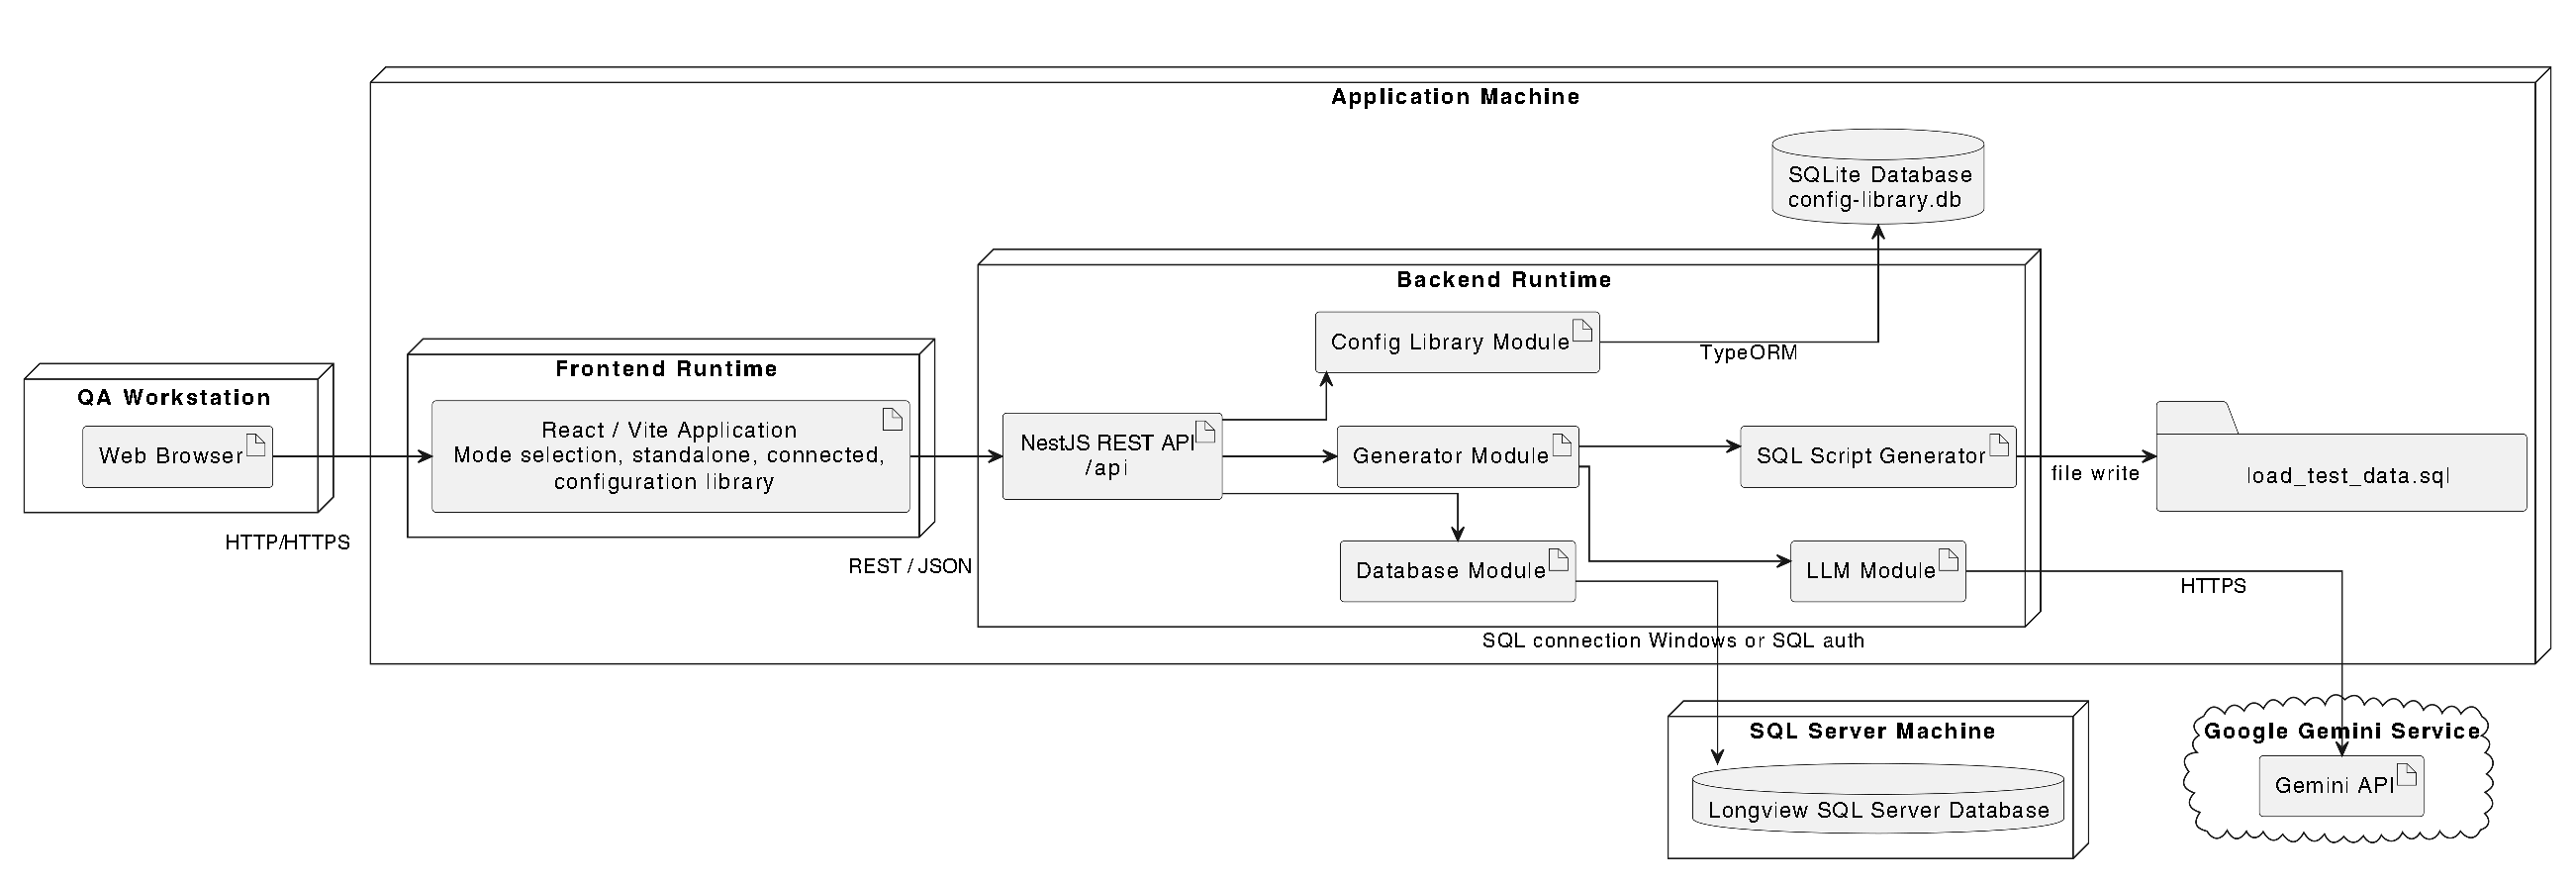
\includegraphics[width=1\textwidth,height=0.84\textheight,keepaspectratio]{img/arch-physical.pdf}}
\caption{Physical architecture of the test data generator}
\label{fig:arch-physical}
\end{figure}


% ─────────────────────────────────────────────
\section{Product Backlog and Sprint Planning}
% ─────────────────────────────────────────────

\paragraph{}The product backlog captures all user stories identified during
the analysis phase, prioritized in collaboration with the Product Owner.
Each user story is expressed from the perspective of the QA engineer or the
system actor that benefits from it. The detailed breakdown of tasks for each
story is presented at the beginning of the corresponding sprint chapter.
Table~\ref{tab:backlog} presents the global product backlog.

\begin{longtable}{|Q{0.08\textwidth}|P{4cm}|P{8.5cm}|}
\caption{Product backlog}
\label{tab:backlog} \\
\hline
\textbf{ID} & \textbf{User Story} & \textbf{Description} \\
\hline
\endfirsthead

\multicolumn{3}{r}{\tablename\ \thetable{} -- \textit{continued from previous page}} \\
\hline
\textbf{ID} & \textbf{User Story} & \textbf{Description} \\
\hline
\endhead

\hline
\multicolumn{3}{r}{\textit{continued on next page}} \\
\endfoot

\hline
\endlastfoot

1 & Generation Parameter Configuration
  & As a QA engineer, I want to configure generation parameters through
    a web form so that I can control entity types, counts, date ranges,
    and operating mode without editing any file. \\
\hline
2 & Account and Account Group Generation
  & As a QA engineer, I want to generate accounts, account groups, and
    hierarchy records so that I can test the full account structure
    loading pipeline. \\
\hline
3 & Model Generation
  & As a QA engineer, I want to generate investment model and
    model-objective records so that I can test model-driven
    allocation scenarios. \\
\hline
4 & Equity and Generic Security Generation
  & As a QA engineer, I want to generate equity and generic instrument
    records so that I can test the loading of basic security types. \\
\hline
5 & Fixed Income Security Generation
  & As a QA engineer, I want to generate fixed income securities along
    with their call, put, coupon, and convertible schedules so that I
    can test the full bond loading pipeline. \\
\hline
6 & Derivative Security Generation
  & As a QA engineer, I want to generate options, futures, and FX
    forward records so that I can test the loading of derivative
    instruments. \\
\hline
7 & Price Generation
  & As a QA engineer, I want to generate price records consistent with
    the generated securities so that I can test the pricing
    load pipeline. \\
\hline
8 & Order and Execution Generation
  & As a QA engineer, I want to generate proposed orders and execution
    records anchored to existing securities and accounts so that I can
    test the full order lifecycle pipeline. \\
\hline
9 & Position Generation
  & As a QA engineer, I want to generate tax-lot position records
    consistent with executed orders so that I can test the position
    loading pipeline. \\
\hline
10 & SQL Script Assembly and Download
  & As a QA engineer, I want the system to assemble and deliver a
    complete, executable SQL script so that I can load all generated
    data into Longview with a single file. \\
\hline
11 & Connected Mode
  & As a QA engineer, I want to connect to a live Longview instance
    in read-only mode so that I can anchor generated records to
    existing database entities. \\
\hline
12 & LLM Enrichment
  & As a QA engineer, I want to enable AI-assisted generation so that
    security names, ticker symbols, and descriptions are realistic
    and contextually meaningful. \\
\hline
13 & Configuration Library
  & As a QA engineer, I want to save and reload named generation
    configurations so that I do not have to re-enter parameters at
    every session. \\
\hline
14 & Validation and Error Handling
  & As a QA engineer, I want the interface to validate my inputs and
    display clear error messages so that I can correct mistakes before
    triggering generation. \\
\hline

\end{longtable}

\paragraph{}The 14 user stories are distributed across five sprints as
shown in Figure~\ref{fig:sprint-plan}. The detailed task breakdown for each
sprint is presented at the beginning of the corresponding implementation
chapter.


% ─────────────────────────────────────────────
\section{Technical Environment}
% ─────────────────────────────────────────────

\paragraph{}The technology choices reflect both the system requirements and
the constraints of the internship environment, covering the full development
chain from the user interface down to the database layer.


% ─────────────────────────────────────────────
\subsection{Hardware}
% ─────────────────────────────────────────────

\paragraph{}Development was carried out on a standard workstation provided
by Linedata Tunisia, running Windows 11. The machine hosted both the
frontend and backend development servers locally and provided connectivity
to the SQL Server instances available in the team's development environment.


% ─────────────────────────────────────────────
\subsection{Software and Technologies}
% ─────────────────────────────────────────────

\paragraph{}In this project, we used the following technologies and tools:


% ── React ──────────────────────────────────────
\paragraph{}\textbf{React 18 + TypeScript}\\
React is an open-source JavaScript library for building user interfaces
through reusable components. Combined with TypeScript, it provides strong
static typing that reduces runtime errors and improves code maintainability.
React was chosen for the frontend of this project due to its component-based
architecture and its suitability for building form-heavy, interactive
interfaces such as the generation parameter configuration panel.
\begin{figure}[H]
\centering

\includegraphics[width=0.12\textwidth]{img/logo-react.png}
\caption{React logo}
\label{fig:logo-react}
\end{figure}


% ── Tailwind CSS ───────────────────────────────
\paragraph{}\textbf{Tailwind CSS + shadcn/ui}\\
Tailwind CSS is a utility-first CSS framework that enables rapid and
consistent UI development directly in markup, without writing custom
stylesheets. It was complemented by shadcn/ui, a collection of accessible
and composable UI components built on top of Radix UI primitives, which
provided ready-made form controls, dialogs, and layout elements consistent
with the application's design system.
\begin{figure}[H]
\centering

\includegraphics[width=0.12\textwidth]{img/logo-tailwind.png}
\caption{Tailwind CSS logo}
\label{fig:logo-tailwind}
\end{figure}


% ── Vite ───────────────────────────────────────
\paragraph{}\textbf{Vite}\\
Vite is a modern frontend build tool that provides an extremely fast
development server through native ES module support, as well as optimized
production builds. It was selected as the build tool for the React frontend
due to its near-instant cold start and hot module replacement, which
significantly improved the development experience.
\begin{figure}[H]
\centering

\includegraphics[width=0.12\textwidth]{img/logo-vite.png}
\caption{Vite logo}
\label{fig:logo-vite}
\end{figure}


% ── NestJS ─────────────────────────────────────
\paragraph{}\textbf{NestJS + TypeScript}\\
NestJS is a progressive Node.js framework for building efficient and
scalable server-side applications. Its modular, decorator-based architecture
maps naturally to the service-per-entity design of the generation engine,
where each entity type (securities, accounts, orders, executions, positions)
is encapsulated in its own dedicated service module. TypeScript support is
first-class and shares the same type definitions with the frontend.
\begin{figure}[H]
\centering

\includegraphics[width=0.12\textwidth]{img/logo-nestjs.png}
\caption{NestJS logo}
\label{fig:logo-nestjs}
\end{figure}


% ── Node.js ────────────────────────────────────
\paragraph{}\textbf{Node.js}\\
Node.js is an open-source, cross-platform JavaScript runtime environment
that executes JavaScript code outside of a browser, on the server side.
It serves as the runtime underlying the NestJS backend, enabling
non-blocking I/O operations that are well-suited for handling concurrent
API requests during generation.
\begin{figure}[H]
\centering

\includegraphics[width=0.12\textwidth]{img/logo-nodejs.png}
\caption{Node.js logo}
\label{fig:logo-nodejs}
\end{figure}


% ── SQL Server ─────────────────────────────────
\paragraph{}\textbf{Microsoft SQL Server + node-mssql}\\
Microsoft SQL Server is the relational database management system underlying
all Longview deployments. It is the target platform for the generated SQL
scripts. The \texttt{node-mssql} package was used as the Node.js driver to
establish the read-only connection in connected mode, offering connection
pooling and parameterized query support.
\begin{figure}[H]
\centering

\includegraphics[width=0.12\textwidth]{img/logo-sqlserver.png}
\caption{Microsoft SQL Server logo}
\label{fig:logo-sqlserver}
\end{figure}


% ── TypeORM + SQLite ───────────────────────────
\paragraph{}\textbf{TypeORM + SQLite (better-sqlite3)}\\
TypeORM is an object-relational mapper for TypeScript and Node.js that
supports multiple database drivers and integrates natively with NestJS
through decorator-based entity definitions. It was used to manage the
\texttt{SavedConfig} entity with automatic schema synchronization, which
eliminates the need for manual migration scripts in the development context.
The \texttt{better-sqlite3} driver was selected as the underlying database
    engine because SQLite is self-contained and serverless -- the database is
stored as a single local file (\texttt{config-library.db}) that TypeORM
creates automatically on first startup, requiring zero infrastructure from
the user.
\begin{figure}[H]
\centering

\includegraphics[width=0.12\textwidth]{img/logo-typeorm.png}
\caption{TypeORM logo}
\label{fig:logo-typeorm}
\end{figure}


% ── Gemini API ─────────────────────────────────
\paragraph{}\textbf{Google Gemini API}\\
Google Gemini is a family of large language models developed by Google
DeepMind. Its REST API was integrated as the LLM enrichment layer of the
generation engine, tasked with producing realistic security names, ticker
symbols, and financial descriptions from structured prompts. An algorithmic
fallback ensures the system remains fully functional when the API is
unavailable.
\begin{figure}[H]
\centering

\includegraphics[width=0.12\textwidth]{img/logo-gemini.png}
\caption{Google Gemini API logo}
\label{fig:logo-gemini}
\end{figure}


% ── Git + GitHub ───────────────────────────────
\paragraph{}\textbf{Git + GitHub}\\
Git is the standard distributed version control system used to track all
changes across the project. GitHub was used as the remote repository
host, enabling branch management, commit history tracking, and sprint-level
progress visibility throughout the internship.
\begin{figure}[H]
\centering

\includegraphics[width=0.12\textwidth]{img/logo-github.png}
\caption{GitHub logo}
\label{fig:logo-github}
\end{figure}


% ── VS Code ────────────────────────────────────
\paragraph{}\textbf{Visual Studio Code}\\
Visual Studio Code is a lightweight and highly extensible source-code
editor developed by Microsoft. It was used as the primary IDE throughout
the project, leveraging extensions for TypeScript IntelliSense, NestJS
snippets, ESLint, Prettier, and the REST Client for API testing directly
within the editor.
\begin{figure}[H]
\centering

\includegraphics[width=0.12\textwidth]{img/logo-vscode.png}
\caption{Visual Studio Code logo}
\label{fig:logo-vscode}
\end{figure}


% ─────────────────────────────────────────────
\section*{Conclusion}
\addcontentsline{toc}{section}{Conclusion}
% ─────────────────────────────────────────────

\paragraph{}This chapter covered the full analysis and design process that
laid the foundation of the project. We adopted Scrum as the development
framework and organized the work into five incremental sprints. A review of
existing test data generation tools confirmed that none of them could address
the specificity of the Longview context, validating the need for a
purpose-built solution. From the functional and non-functional requirements,
we derived a layered architecture built around a React frontend, a NestJS
backend with entity-specific generation services, a Gemini API integration
for data realism, a read-only SQL Server connection for connected mode, and
a local SQLite persistence layer that allows QA engineers to save and reload
named generation configurations across sessions. This design was documented
through a global use case diagram, a global package diagram, and a physical
architecture diagram, each covering a distinct view of the system. The 14 user stories
organized in the product backlog and distributed across five sprints gave
the implementation a clear and structured roadmap. The next chapter covers
Sprint 1, the discovery phase in which the existing SQL scripts were analyzed
and the Longview data model was fully mapped in preparation for the
generation engine.

        \clearpage
        
        \chapter{Sprint 1 -- Discovery and Data Model Mapping}

% ---------------------------------------------------------
\section*{Introduction}
\addcontentsline{toc}{section}{Introduction}
% ---------------------------------------------------------

\paragraph{}This chapter presents the first sprint of the project, which spanned two weeks. Its purpose was not to
implement the generator yet, but to clarify the financial and technical rules needed before
implementation. Since the application produces data for Longview, the sprint identified the meaning
of the main entities to generate, their dependencies, and the constraints that must be respected by
the later SQL generation pipeline.


% ---------------------------------------------------------
\section{Sprint Backlog}
% ---------------------------------------------------------

\paragraph{}Sprint 1 targeted user story \textbf{US-1}, dedicated to discovering and documenting the
Longview data model before starting the generation engine. The sprint backlog is presented in
Table~\ref{tab:sprint1-backlog}.

\Needspace{12\baselineskip}
\renewcommand{\arraystretch}{1.35}
\begin{longtable}{|Q{0.08\textwidth}|P{0.28\textwidth}|P{0.42\textwidth}|Q{0.12\textwidth}|}
\caption{Sprint 1 backlog}
\label{tab:sprint1-backlog} \\
\hline
\textbf{ID} & \textbf{Task} & \textbf{Description} & \textbf{Estimate} \\
\hline
\endfirsthead
\multicolumn{4}{r}{\tablename\ \thetable{} -- \textit{continued from previous page}} \\
\hline
\textbf{ID} & \textbf{Task} & \textbf{Description} & \textbf{Estimate} \\
\hline
\endhead
\hline
\multicolumn{4}{r}{\textit{continued on next page}} \\
\endfoot
\hline
\endlastfoot
T1-1 & Review existing SQL and extract files & Identify the files used by the QA team, the tables they populate, and the business entities behind them. & 2 days \\
\hline
T1-2 & Study pre-BCP buffer tables & Document the columns, mandatory fields, keys, and identity columns required by the Longview loading layer. & 3 days \\
\hline
T1-3 & Map stored procedures and load order & Identify the loading procedures and the dependency order that must be respected when generating SQL. & 2 days \\
\hline
T1-4 & Extract business rules & Collect the main financial constraints, code lists, and referential rules used to validate the generated records. & 2 days \\
\hline
T1-5 & Produce entity diagrams & Consolidate the discovered entities, attributes, and relationships into UML class diagrams. & 1 day \\
\end{longtable}

% ---------------------------------------------------------
\section{Sprint Specification}
% ---------------------------------------------------------

\paragraph{}The specification work of Sprint 1 transformed existing Longview material into a clear
generation scope. The sprint identified which business entities had to be generated, how they depend
on each other, and which rules must be preserved by the later generation engine.

\subsection{Target Entity Scope}

\paragraph{}Since Longview contains many extract files, Sprint 1 first reduced the scope to the data
most useful for QA scenarios. Existing extract files, manually written SQL scripts, and QA feedback
were analyzed to identify the entities that are frequently needed, strongly dependent on each other,
and difficult to create manually. The selected scope covers accounts and account groups, models,
securities, prices, hierarchy rows, positions, proposed orders, orders, and executions.

\subsection{Financial Concept Mapping}

\paragraph{}The selected extracts were mapped to the main financial concepts needed by QA
scenarios. This mapping, summarized in Table~\ref{tab:finance-map}, helped separate the business
meaning of each entity from its role in the generator.

\Needspace{10\baselineskip}
\renewcommand{\arraystretch}{1.3}
\begin{longtable}{|P{0.22\textwidth}|P{0.34\textwidth}|P{0.34\textwidth}|}
\caption{Reader's map of the main financial concepts}
\label{tab:finance-map} \\
\hline
\textbf{Concept} & \textbf{Finance meaning} & \textbf{Role in the generator} \\
\hline
\endfirsthead
\multicolumn{3}{r}{\tablename\ \thetable{} -- \textit{continued from previous page}} \\
\hline
\textbf{Concept} & \textbf{Finance meaning} & \textbf{Role in the generator} \\
\hline
\endhead
\hline
\multicolumn{3}{r}{\textit{continued on next page}} \\
\endfoot
\hline
\endlastfoot
Account & A client portfolio or investment account. & Main owner of positions, proposed orders, orders, and optional executions. \\
\hline
Account Group & A business grouping of accounts. & Adds hierarchy and reporting structure around generated accounts. \\
\hline
Model & A target allocation strategy. & Provides allocation data and optional model references for account scenarios. \\
\hline
Security & A tradeable financial instrument such as an equity, bond, option, future, generic instrument, or FX forward. & Central reference reused by prices, hierarchy rows, positions, orders, and executions. \\
\hline
Price & The market value of a security. & Allows generated securities to be valued by Longview. \\
\hline
Position & What an account already owns. & Gives the generator holding context, especially for sell-side order scenarios. \\
\hline
Proposed Order / Order & An intention to trade and the actual trading instruction. & Creates trading activity for valid account-security pairs. \\
\hline
Execution & A market fill confirming that a trade was executed. & Completes the trade lifecycle for generated equity orders. \\
\hline
\end{longtable}

% ---------------------------------------------------------
\subsection{Entity Relationships}
% ---------------------------------------------------------

\paragraph{}After selecting the target extracts, Sprint 1 mapped the relationships required for valid
generation. Prices must reference securities, positions must connect accounts with securities, and
orders must reuse valid account-security pairs. Additional generation rules were also identified, such
as linking options to an underlying security and producing executions from equity orders. This mapping
became the basis for the DTO design and for the later generation pipeline, where services share
generated identifiers instead of producing each output independently.

% ---------------------------------------------------------
\section{Sprint Design}
% ---------------------------------------------------------

\paragraph{}After the sprint specification defined the target entities and their relationships, the
design work focused on how these entities must be loaded by Longview. This design step produced
the pre-BCP loading model, the technical population order, and the UML diagrams used as reference
models for the following sprints.

\subsection{Longview Pre-BCP Loading Mechanism}

\paragraph{}Sprint 1 also clarified the Longview loading mechanism. Generated records are first
inserted into pre-BCP buffer tables, then Longview stored procedures validate them, apply business
rules, and transfer the accepted data into the live schema. Therefore, the generated SQL must target
the buffer tables and respect the required population order, so each referenced account, security,
model, or classification level exists before it is used.

% ---------------------------------------------------------
\subsection{Table Population Order}
% ---------------------------------------------------------

\paragraph{}After understanding the pre-BCP mechanism, the next step was to determine the order
in which the application must write the generated records. This order is used by the SQL script
generator when it emits \texttt{INSERT} statements, identity-column handling blocks, and stored
procedure calls.

\paragraph{}Table~\ref{tab:population-order} summarizes the selected pre-BCP loading order used
by the application. It follows the technical dependency sequence required by Longview.

\Needspace{14\baselineskip}
\renewcommand{\arraystretch}{1.3}
\begin{longtable}{|Q{0.08\textwidth}|P{0.40\textwidth}|P{0.42\textwidth}|}
\caption{Pre-BCP buffer table population order}
\label{tab:population-order} \\
\hline
\textbf{Step} & \textbf{Entity} & \textbf{Dependency} \\
\hline
\endfirsthead
\multicolumn{3}{r}{\tablename\ \thetable{} -- \textit{continued from previous page}} \\
\hline
\textbf{Step} & \textbf{Entity} & \textbf{Dependency} \\
\hline
\endhead
\hline
\multicolumn{3}{r}{\textit{continued on next page}} \\
\endfoot
\hline
\endlastfoot
1 & Security masters: Equity, Fixed Income, Future, Generic and FX Forward & Base security universe. \\
\hline
2 & Option security & Generated after equities and futures because options need an underlying security. \\
\hline
3 & Fixed-income schedules: CALL,PUT,COUP,CONVERT & Fixed income parent security. \\
\hline
4 & Hierarchy & Generated securities and classification definitions. \\
\hline
5 & Price & Security identifiers, including synthetic FX forward identifiers. \\
\hline
6 & Model properties & Generated model names used by model allocations and optional account references. \\
\hline
7 & Model allocations  & Model names from the generated model property records. \\
\hline
8 & Model of Models & Existing parent and submodel identifiers. \\
\hline
9 & Account & No mandatory generated dependency; optional references must already exist when populated. \\
\hline
10 & Account Group & Account membership through \textbf{client\_account\_id}. \\
\hline
11 & Position & Account and security. Generated before orders to support coherent sell scenarios. \\
\hline
12 & Proposed Order & Account, security, and current position context. \\
\hline
13 & Order & Same row shape as proposed orders, loaded with the appropriate Longview procedure mode. \\
\hline
14 & Execution  & Generated from equity orders only; references security and account when supplied. \\
\hline
\end{longtable}

\paragraph{}This order differs from the explanatory business sequence because the SQL script must
satisfy Longview dependencies. The generator therefore creates a coherent business scenario while
emitting SQL in the order accepted by the pre-BCP pipeline.

% ---------------------------------------------------------
\subsection{Entity Class Diagrams}
% ---------------------------------------------------------

\paragraph{}Figure~\ref{fig:class-diagram} presents the UML class diagram produced at the end of
Sprint 1. It served as the reference for the DTO classes and for the generation services implemented
in the following sprint.

\begin{figure}[H]
\centering
\makebox[\textwidth][c]{%
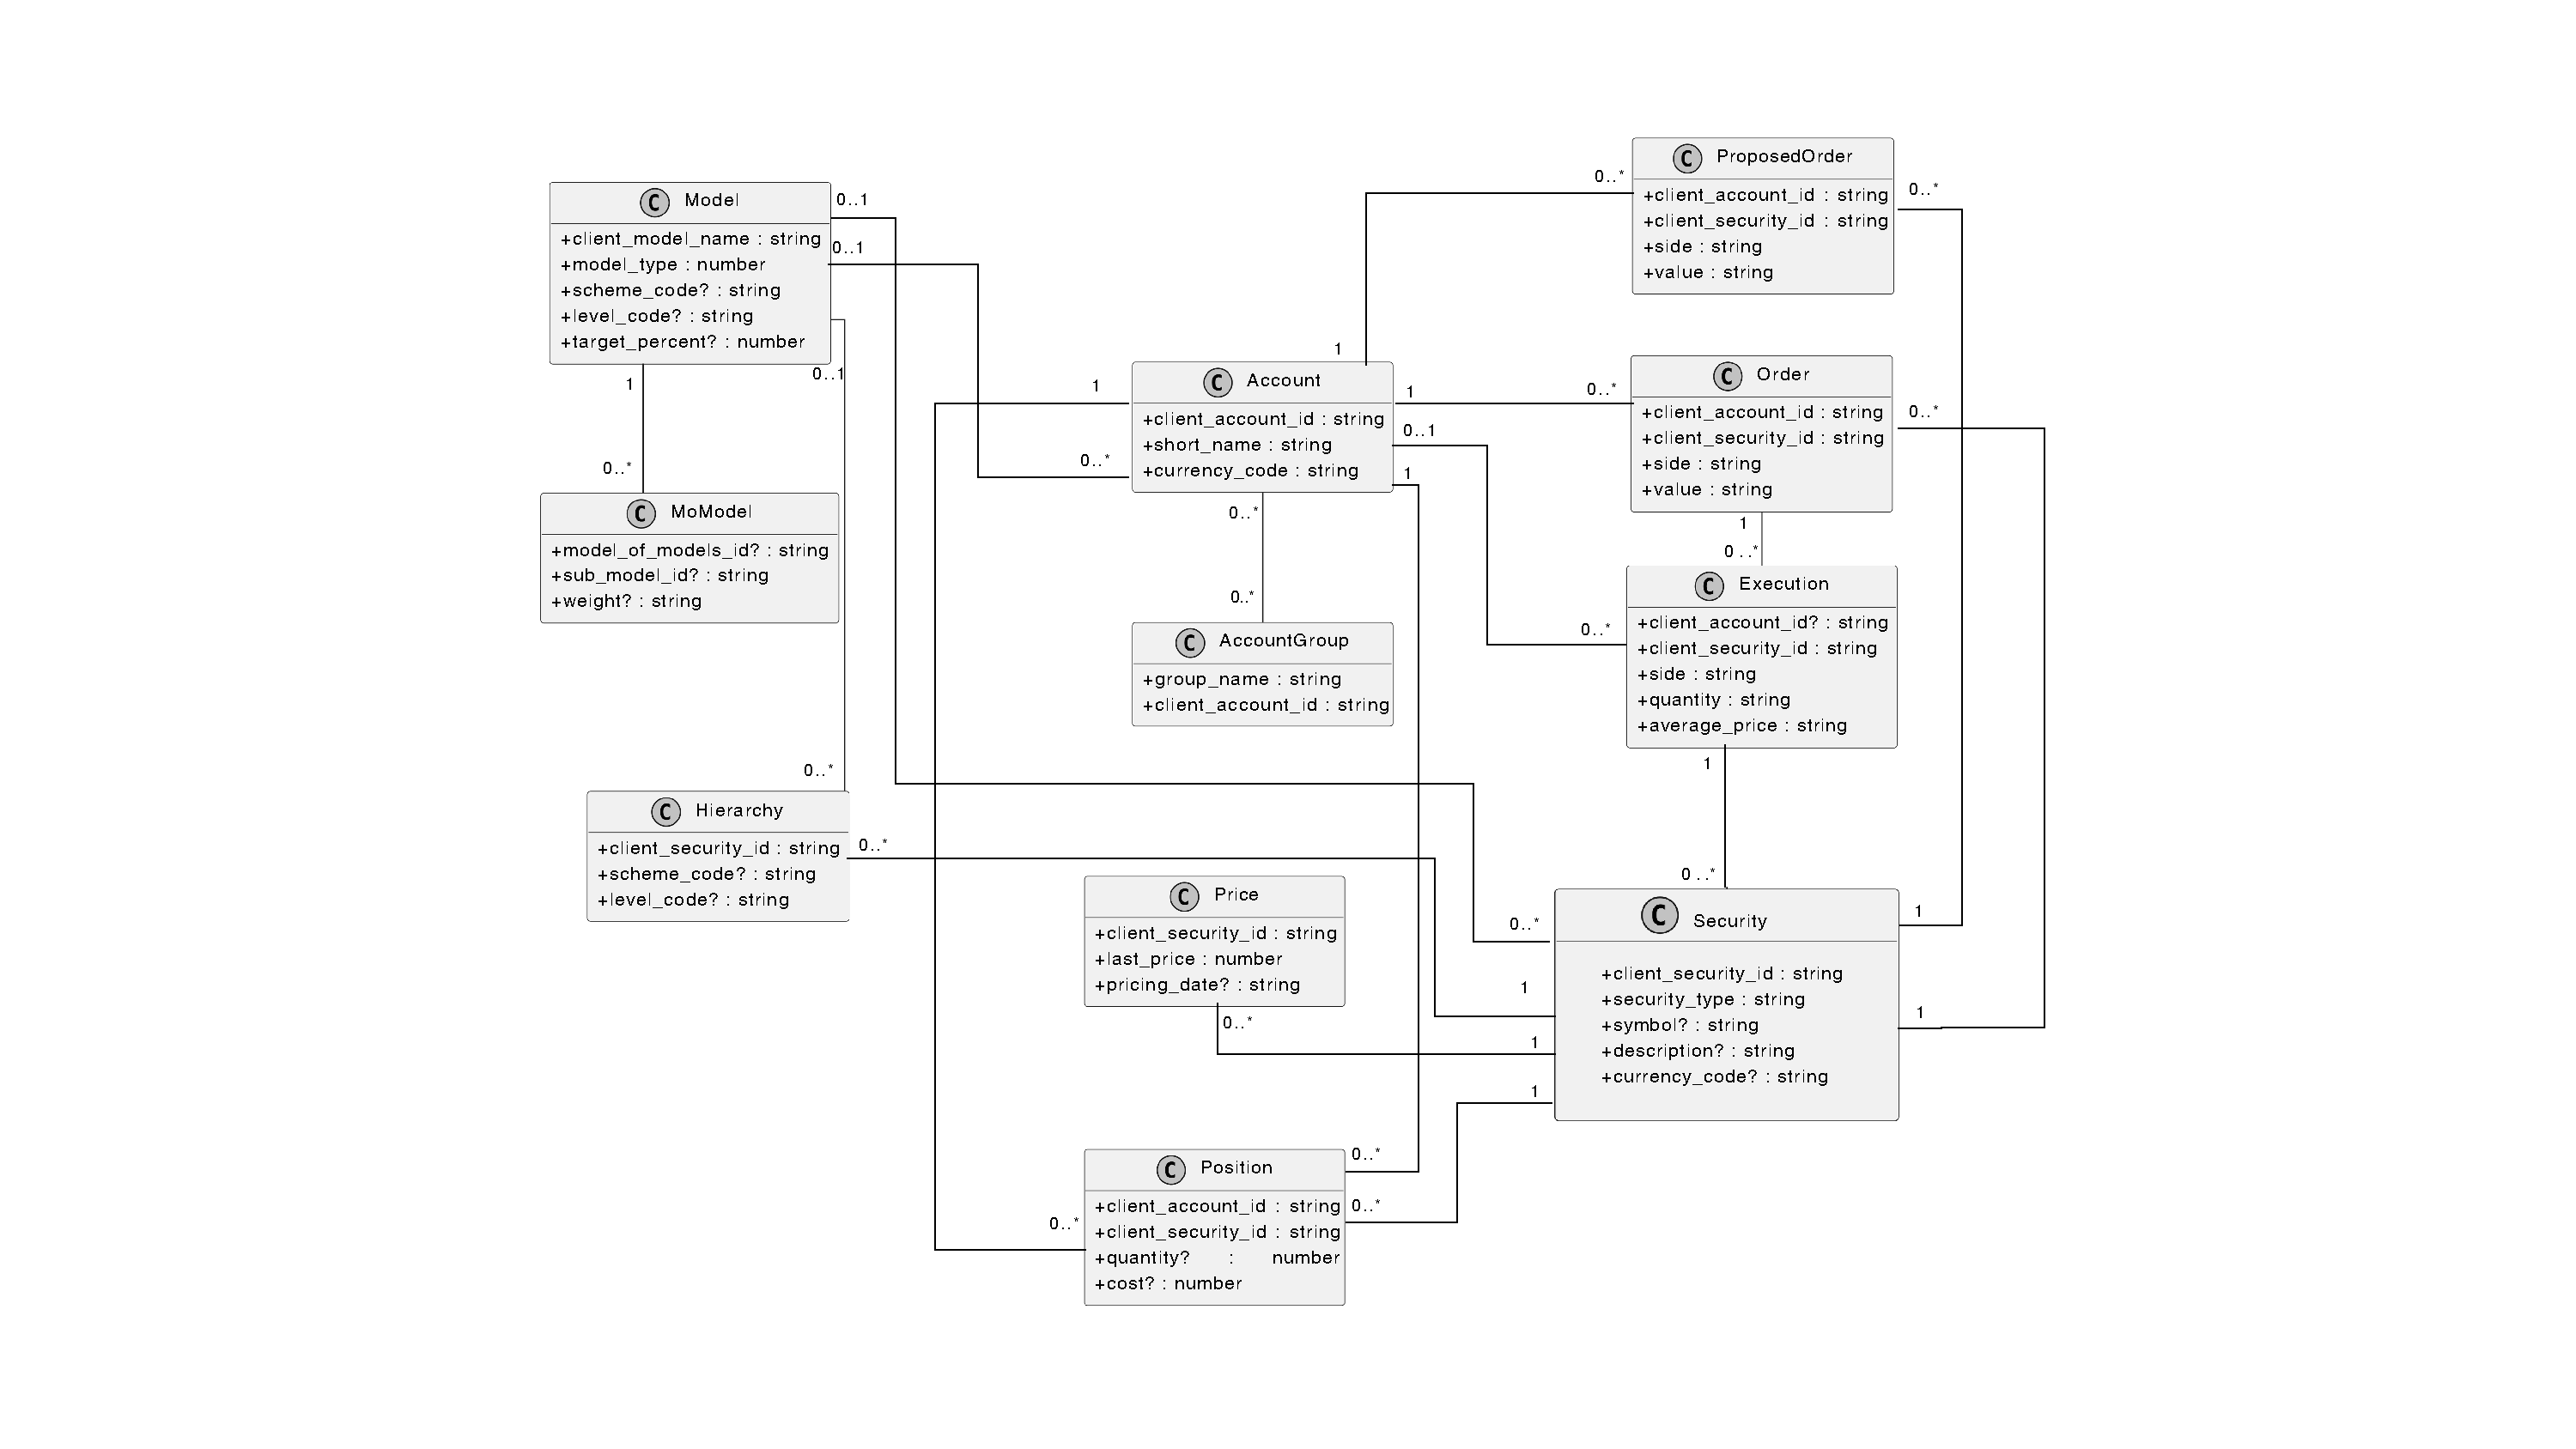
\includegraphics[width=1.5\textwidth,height=0.78\textheight,keepaspectratio]{img/classdiagram-entities.pdf}%
}
\caption{UML class diagram of the Longview entities targeted by the test data generator}
\label{fig:class-diagram}
\end{figure}

\paragraph{}Because securities are the most specialized part of the model, Figure~\ref{fig:security-class-diagram}
isolates the security DTO hierarchy. This separation was needed because each subtype has its own
fields and validation rules.

\begin{figure}[H]
\centering
\makebox[\textwidth][c]{%
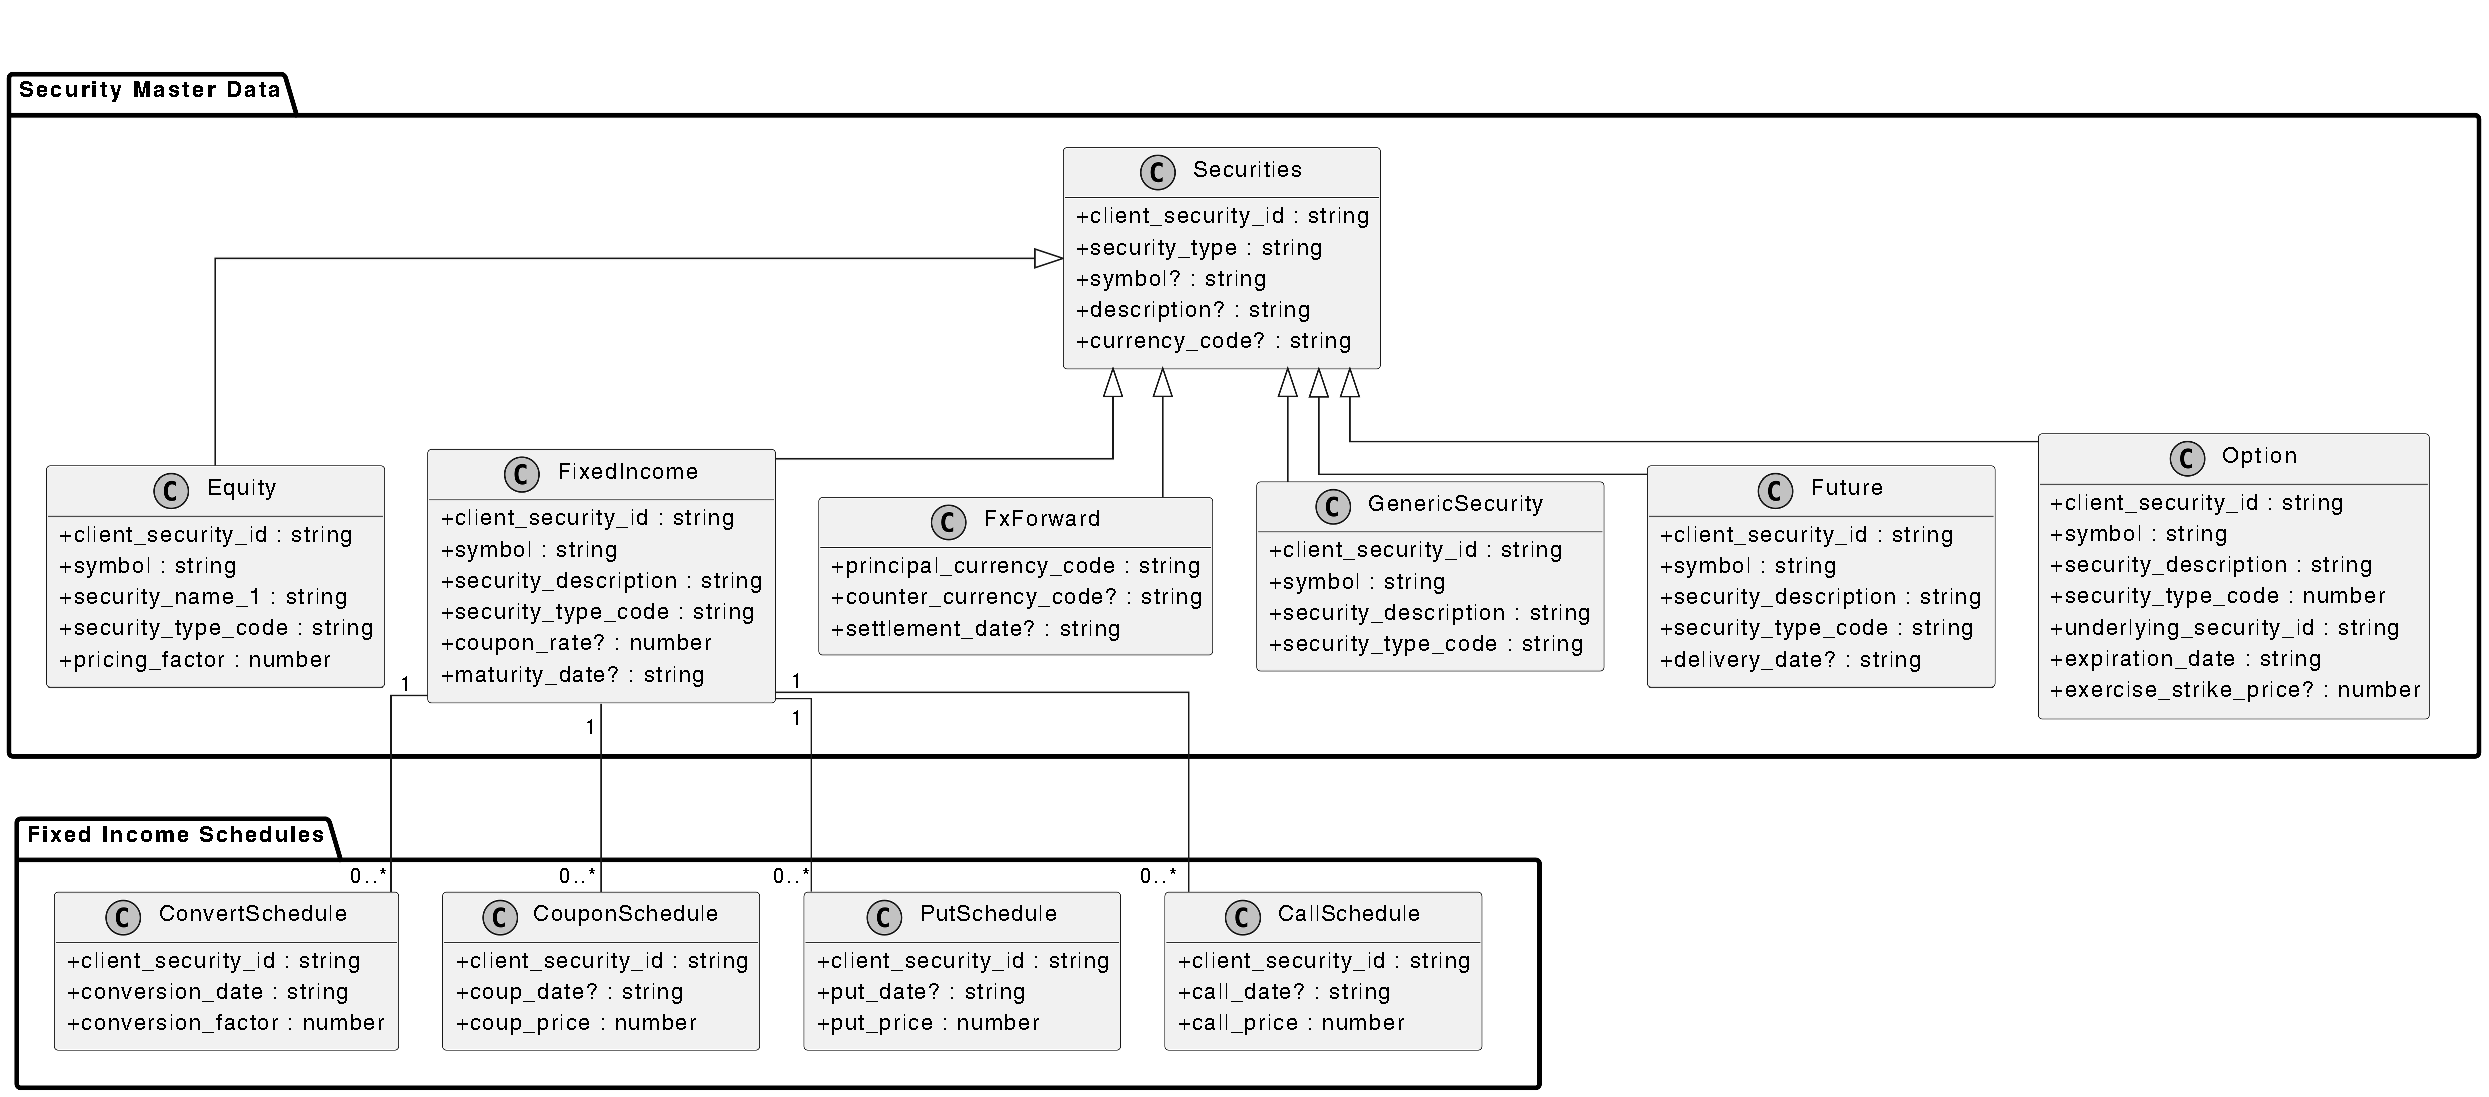
\includegraphics[width=1\textwidth,height=0.78\textheight,keepaspectratio]{img/classdiagram-securities.pdf}%
}
\caption{UML class diagram of the security DTO hierarchy}
\label{fig:security-class-diagram}
\end{figure}

% ---------------------------------------------------------
\section{Realization}
% ---------------------------------------------------------

\paragraph{}The realization of Sprint 1 produced the reference material used before implementation:
the selected entity scope, the relationship rules, the pre-BCP population order, and the UML class
diagrams. The main practical outcome was the separation between the business scenario to generate
and the technical order required by Longview.

\paragraph{}Table~\ref{tab:sprint1-deliverables} summarizes the concrete deliverables produced at
the end of the sprint and explains how each one was reused during the following implementation
sprints.

\Needspace{12\baselineskip}
\renewcommand{\arraystretch}{1.3}
\begin{longtable}{|P{0.28\textwidth}|P{0.31\textwidth}|P{0.31\textwidth}|}
\caption{Sprint 1 realization deliverables}
\label{tab:sprint1-deliverables} \\
\hline
\textbf{Deliverable} & \textbf{Produced result} & \textbf{Use in the project} \\
\hline
\endfirsthead
\multicolumn{3}{r}{\tablename\ \thetable{} -- \textit{continued from previous page}} \\
\hline
\textbf{Deliverable} & \textbf{Produced result} & \textbf{Use in the project} \\
\hline
\endhead
\hline
\multicolumn{3}{r}{\textit{continued on next page}} \\
\endfoot
\hline
\endlastfoot
Selected extracts & Accounts, account groups, models, securities, prices, positions, proposed orders, orders, and executions were selected as the initial generation scope. & Defined the functional perimeter of the standalone generator. \\
\hline
Entity mapping & Each selected business concept was linked to its corresponding DTO, extract file, and pre-BCP buffer table. & Guided the backend DTO structure and generation services. \\
\hline
Relationship rules & Mandatory and optional references between accounts, securities, prices, positions, orders, executions, and models were identified. & Used later by the relationship validation layer. \\
\hline
Population order & The technical loading sequence of the pre-BCP files was established. & Used by the SQL script generation step to emit loadable data in the correct order. \\
\hline
Class diagrams & Entity and security DTO diagrams were produced. & Served as the modeling reference for the implementation of the generation engine. \\
\hline
\end{longtable}
\renewcommand{\arraystretch}{1}

\paragraph{}A screenshot of the analyzed extract folder or an annotated mapping sheet can be added
later in Figure~\ref{fig:sprint1-extract-analysis-proof} to visually document the discovery work
performed during this sprint.

\begin{figure}[H]
\centering
\IfFileExists{img/ch3-extract-analysis-proof.png}{%
    \includegraphics[width=0.88\textwidth]{img/ch3-extract-analysis-proof.png}%
}{%
    \fbox{\parbox[c][0.22\textheight][c]{0.86\textwidth}{\centering Screenshot to be added: selected extracts, mapping sheet, or analyzed SQL files}}%
}
\caption{Sprint 1 extract analysis and mapping evidence}
\label{fig:sprint1-extract-analysis-proof}
\end{figure}

% ---------------------------------------------------------
\section*{Conclusion}
\addcontentsline{toc}{section}{Conclusion}
% ---------------------------------------------------------

\paragraph{}This chapter presented Sprint 1 as the discovery phase that defined the entities,
relationships, loading order, and UML reference models needed before implementation. This
foundation gave Sprint 2 the specification required to build the standalone generation engine and
produce SQL scripts that respect Longview's loading constraints.

        \clearpage
        
        \chapter{Sprint 2 -- Core Generation Engine and Standalone Mode}

\setlength{\textfloatsep}{8pt plus 2pt minus 2pt}
\setlength{\floatsep}{8pt plus 2pt minus 2pt}
\setlength{\intextsep}{8pt plus 2pt minus 2pt}
\setlength{\abovecaptionskip}{4pt}
\setlength{\belowcaptionskip}{0pt}

\section*{Introduction}
\addcontentsline{toc}{section}{Introduction}

\paragraph{}Sprint 1 established what kind of Longview data had to be produced and how the generated
records depend on each other. Sprint 2 represents the first concrete use of that analysis inside the
application. Its objective was to give the QA engineer an autonomous generation mode, able to create
a complete test dataset without requiring access to an existing Longview database.

\paragraph{}The standalone mode is therefore the foundation of the generator. From a configuration
entered in the interface, the application prepares coherent accounts, securities, prices, positions,
orders, executions, and related records, then returns an ordered SQL Server loading script. This
chapter focuses on the realization of that workflow and on the safeguards that make the generated
output usable by a QA engineer.

\section{Sprint Backlog}

\paragraph{}The backlog of Sprint 2 was defined around one objective: allow a QA engineer to configure,
preview, generate, validate, and download a complete SQL loading script without using an existing
Longview database. Table~\ref{tab:sprint2-backlog} presents the tasks selected for this sprint.

\small
\renewcommand{\arraystretch}{1.05}
\begin{longtable}{|Q{0.07\linewidth}|P{0.29\linewidth}|P{0.42\linewidth}|Q{0.12\linewidth}|}
\caption{Sprint 2 backlog}
\label{tab:sprint2-backlog} \\
\hline
\textbf{ID} & \textbf{Task} & \textbf{Description} & \textbf{Estimate} \\
\hline
\endfirsthead
\multicolumn{4}{r}{\tablename\ \thetable{} -- \textit{continued from previous page}} \\
\hline
\textbf{ID} & \textbf{Task} & \textbf{Description} & \textbf{Estimate} \\
\hline
\endhead
\hline
\multicolumn{4}{r}{\textit{continued on next page}} \\
\endfoot
\hline
\endlastfoot
T2-1 & Implement standalone configuration & Build the configuration form for reference date, accounts, securities, orders, positions, models, and executions. & 4 days \\
\hline
T2-2 & Implement dependency rules & Prevent incoherent selections such as executions without orders or dependent data without accounts and securities. & 2 days \\
\hline
T2-3 & Implement preview estimation & Estimate the number of generated records before the final generation request. & 2 days \\
\hline
T2-4 & Implement internal generation services & Generate accounts, account groups, securities, prices, models, positions, proposed orders, orders, and executions from configuration values. & 5 days \\
\hline
T2-5 & Implement validation & Check field formats, required values, numeric values, dates, flags, and relationships between generated records. & 3 days \\
\hline
T2-6 & Implement SQL export & Transform the validated generated records into an ordered SQL Server loading script and return it for download. & 3 days \\
\hline
T2-7 & Add progress and error feedback & Display generation progress, success state, and error state during the generation process. & 2 days \\
\hline
\end{longtable}
\normalsize
\renewcommand{\arraystretch}{1}

\section{Sprint Specification}

\paragraph{}The standalone mode is organized around three main use cases: configuring generation
parameters, viewing the preview, and generating the SQL script.

\subsection{Use Case Refinement}

\paragraph{}Figure~\ref{fig:usecase-standalone} presents the refined standalone use case diagram, while
Table~\ref{tab:sprint2-refined-usecases} summarizes the goal of each refined action.

\begin{figure}[!htbp]
\centering
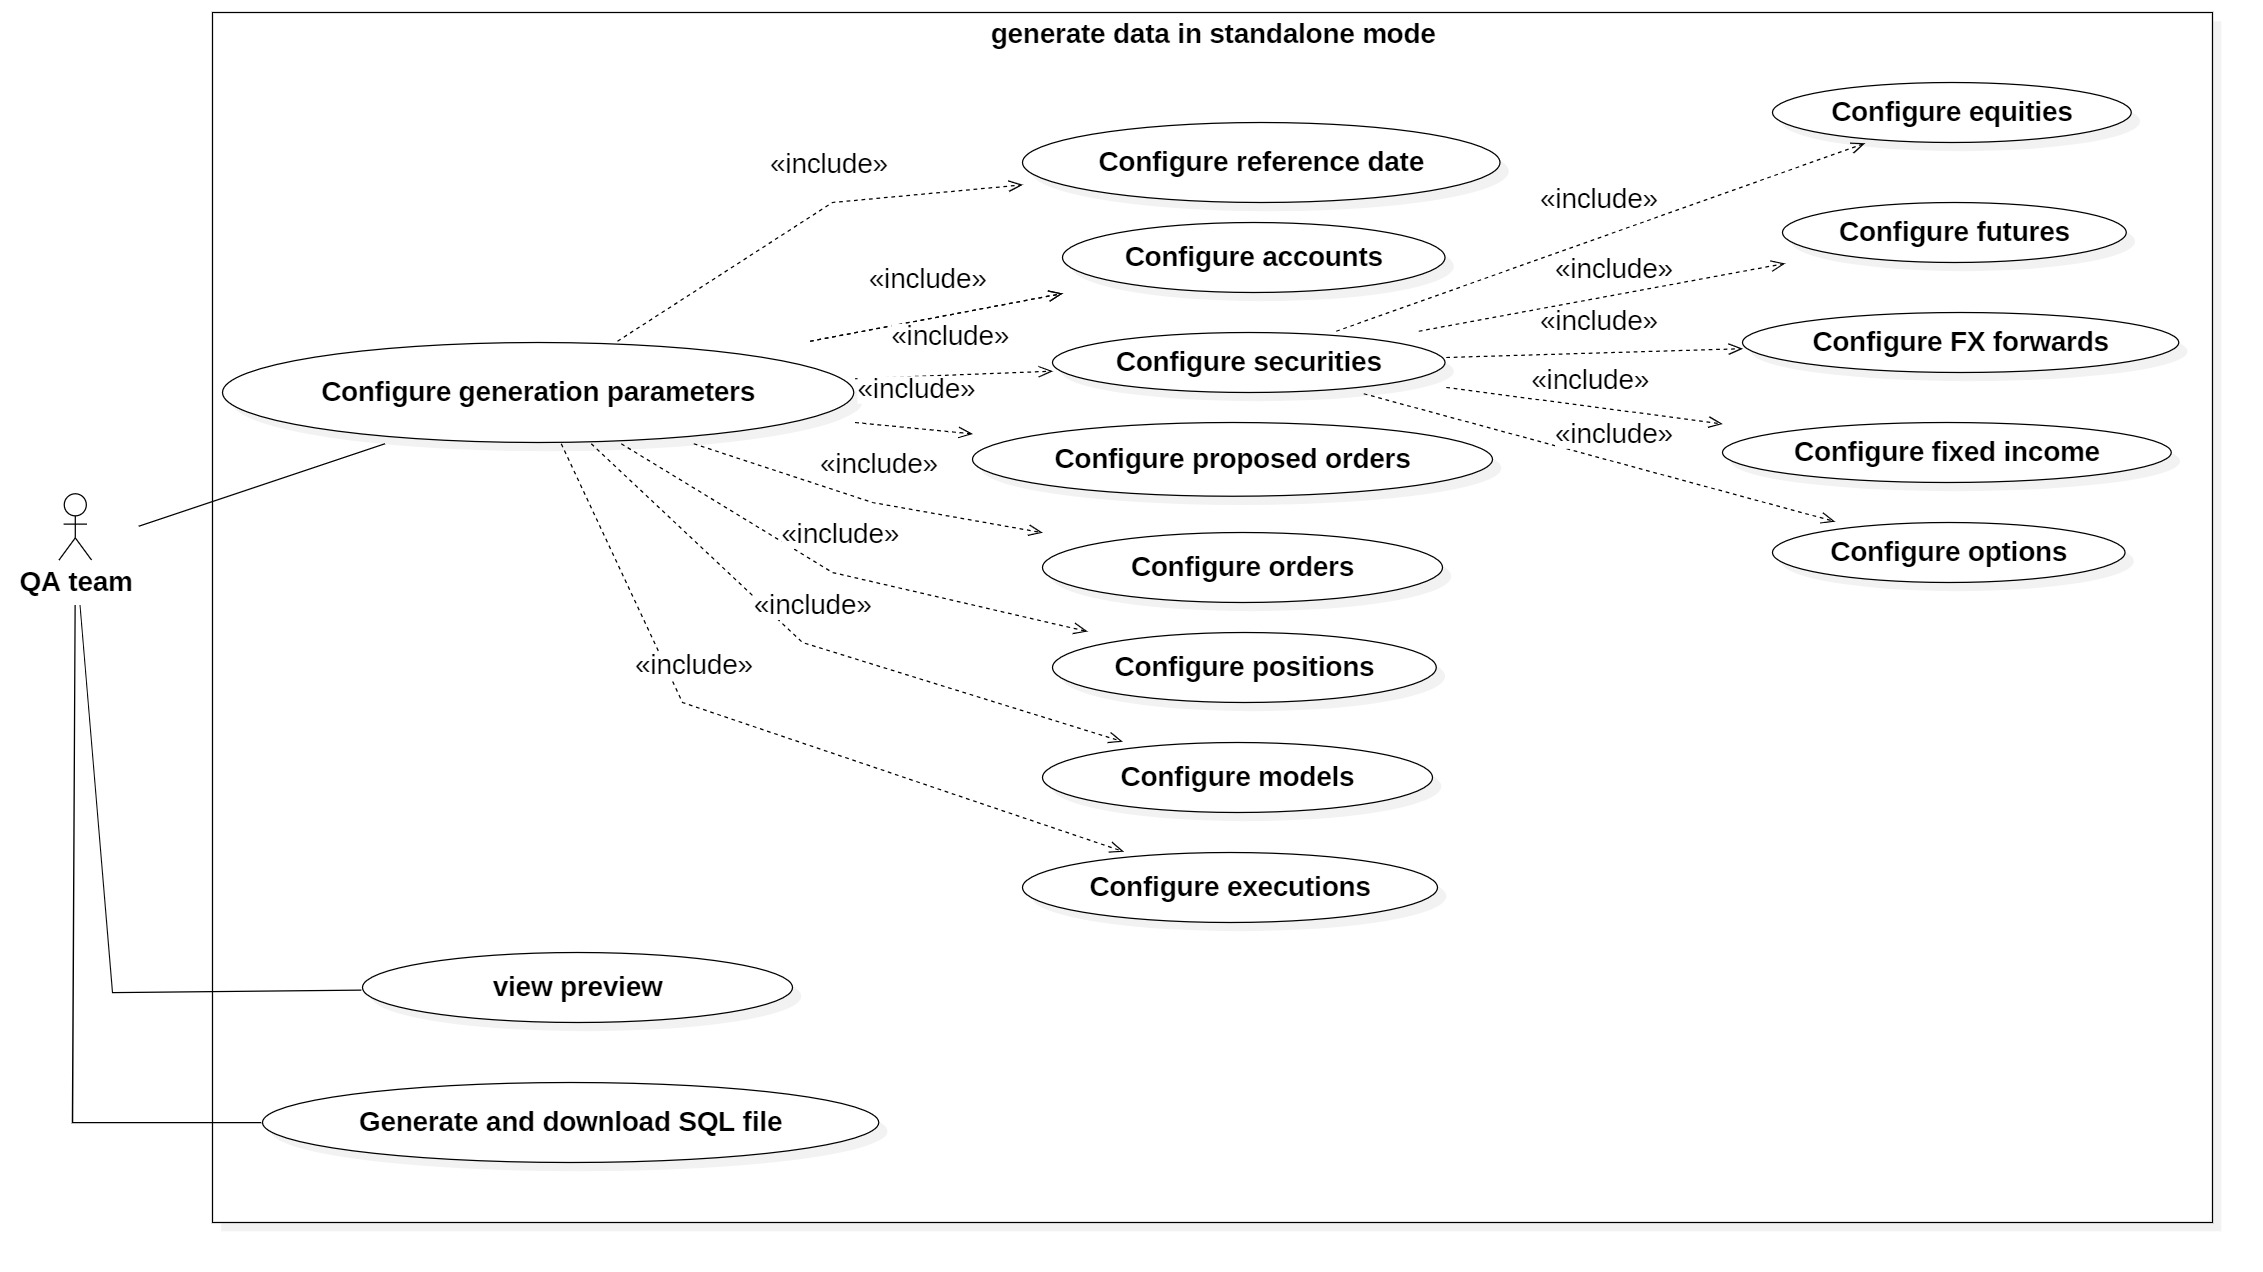
\includegraphics[width=0.95\textwidth]{img/usecase-standalone-mode-clean.jpg}
\caption{Refined use case diagram of standalone mode}
\label{fig:usecase-standalone}
\end{figure}

\renewcommand{\arraystretch}{1.15}
\begin{longtable}{|P{0.27\linewidth}|P{0.23\linewidth}|P{0.40\linewidth}|}
\caption{Refined use cases of Sprint 2}
\label{tab:sprint2-refined-usecases} \\
\hline
\textbf{Refined use case} & \textbf{Actor} & \textbf{Goal} \\
\hline
\endfirsthead
\multicolumn{3}{r}{\tablename\ \thetable{} -- \textit{continued from previous page}} \\
\hline
\textbf{Refined use case} & \textbf{Actor} & \textbf{Goal} \\
\hline
\endhead
\hline
\multicolumn{3}{r}{\textit{continued on next page}} \\
\endfoot
\hline
\endlastfoot
Configure generation parameters & QA Engineer & Define what data must be generated and with which quantities, ranges, ratios, and naming rules. \\
\hline
Configure reference date & QA Engineer & Set the base date used by prices, positions, orders, executions, and generated financial dates. \\
\hline
Configure accounts & QA Engineer & Generate the account universe used by models, positions, orders, and executions. \\
\hline
Configure securities & QA Engineer & Select the instrument types and quantities used by prices, positions, orders, models, and executions. \\
\hline
Configure proposed orders & QA Engineer & Generate proposed trades using accounts, securities, quantity ranges, and buy/sell ratio. \\
\hline
Configure orders & QA Engineer & Generate final orders that can later be used by executions. \\
\hline
Configure positions & QA Engineer & Generate holdings for account-security pairs, with long/short and tax-lot options. \\
\hline
Configure models & QA Engineer & Generate model allocations based on generated accounts and securities. \\
\hline
Configure executions & QA Engineer & Generate fills only when final orders are available. \\
\hline
View preview & QA Engineer & Review estimated record counts before launching generation. \\
\hline
Generate and download SQL script & QA Engineer & Produce and download the SQL Server loading script. \\
\hline
\end{longtable}
\renewcommand{\arraystretch}{1}

\subsection{Textual Use Case Description}

\subsubsection{Configure Generation Parameters}

\paragraph{}Table~\ref{tab:configure-generation-usecase} details the configuration use case and the
guards applied before preview.

\renewcommand{\arraystretch}{1.15}
\begin{longtable}{|P{0.24\linewidth}|P{0.66\linewidth}|}
\caption{Textual description of the configuration use case}
\label{tab:configure-generation-usecase} \\
\hline
\textbf{Element} & \textbf{Description} \\
\hline
\endfirsthead
\multicolumn{2}{r}{\tablename\ \thetable{} -- \textit{continued from previous page}} \\
\hline
\textbf{Element} & \textbf{Description} \\
\hline
\endhead
\hline
\multicolumn{2}{r}{\textit{continued on next page}} \\
\endfoot
\hline
\endlastfoot
Use case & Configure generation parameters. \\
\hline
Actor & QA Engineer. \\
\hline
Preconditions & The QA engineer selected standalone mode and reached the configuration step. \\
\hline
Postconditions & A valid standalone configuration is available for preview and generation. \\
\hline
Main scenario &
\begin{enumerate}[leftmargin=*,nosep]
    \item The QA engineer chooses the reference date.
    \item The QA engineer enables account generation and defines the number of accounts, currency, and naming patterns.
    \item The QA engineer enables security generation and enters quantities for the selected instrument types.
    \item The QA engineer optionally enables proposed orders, final orders, positions, models, and executions.
    \item The system checks dependency rules, disables unavailable dependent sections, and reports invalid values.
    \item The system displays a summary of the selected configuration and enables the next step only when the configuration is valid.
\end{enumerate} \\
\hline
Configuration guards &
\begin{itemize}[leftmargin=*,nosep]
    \item At least one data family, accounts or securities, must be selected.
    \item Proposed orders, final orders, positions, models, and executions require both accounts and securities.
    \item Executions require final orders.
    \item Fixed-income schedules are available only when fixed-income securities are selected.
    \item Quantity and value maximums must be greater than or equal to their minimums.
    \item Generation quantities must remain within the frontend and backend safety limits.
    \item Estimated output above 100,000 rows raises a warning, while output above 500,000 rows blocks generation.
    \item Tax lots require at least two lots per position.
\end{itemize} \\
\hline
Exception scenario &
\begin{itemize}[leftmargin=*,nosep]
    \item If no data is selected, the system displays validation messages and blocks access to preview.
    \item If accounts or securities are not available, the dependent sections are disabled and any already selected dependent options are cleared.
    \item If orders are disabled while executions are enabled, executions are automatically disabled.
    \item If invalid numeric values are entered, the system displays validation messages and blocks access to preview.
    \item If the estimated output exceeds the maximum row budget, the system blocks preview or generation until the configuration is reduced.
\end{itemize} \\
\hline
\end{longtable}
\renewcommand{\arraystretch}{1}

\subsubsection{View Preview}

\paragraph{}Table~\ref{tab:preview-usecase} describes the preview step used to review the estimated
generation result before launching the backend process.

\renewcommand{\arraystretch}{1.15}
\begin{longtable}{|P{0.24\linewidth}|P{0.66\linewidth}|}
\caption{Textual description of the preview use case}
\label{tab:preview-usecase} \\
\hline
\textbf{Element} & \textbf{Description} \\
\hline
\endfirsthead
\multicolumn{2}{r}{\tablename\ \thetable{} -- \textit{continued from previous page}} \\
\hline
\textbf{Element} & \textbf{Description} \\
\hline
\endhead
\hline
\multicolumn{2}{r}{\textit{continued on next page}} \\
\endfoot
\hline
\endlastfoot
Use case & View preview. \\
\hline
Actor & QA Engineer. \\
\hline
Preconditions & The standalone configuration is valid. \\
\hline
Postconditions & The QA engineer can decide whether to return to configuration or launch generation. \\
\hline
Main scenario &
\begin{enumerate}[leftmargin=*,nosep]
    \item The QA engineer opens the preview step.
    \item The frontend estimates generated records from account count, security quantities, selected dependencies, and per-account options.
    \item The system displays a summary of the expected generation result, including the target buffer table and loading procedure for each generated data category.
    \item The QA engineer either returns to configuration or starts generation.
\end{enumerate} \\
\hline
Exception scenario & If the configuration contains missing dependencies or invalid values, the
system disables access to the preview and displays the corresponding validation messages in the
configuration summary. The QA engineer corrects the affected parameters before opening the preview. \\
\hline
\end{longtable}
\renewcommand{\arraystretch}{1}

\subsubsection{Generate and Download SQL Script}

\paragraph{}Table~\ref{tab:generate-sql-usecase} describes the final generation step, from backend
execution to SQL download.

\renewcommand{\arraystretch}{1.15}
\begin{longtable}{|P{0.24\linewidth}|P{0.66\linewidth}|}
\caption{Textual description of the SQL generation use case}
\label{tab:generate-sql-usecase} \\
\hline
\textbf{Element} & \textbf{Description} \\
\hline
\endfirsthead
\multicolumn{2}{r}{\tablename\ \thetable{} -- \textit{continued from previous page}} \\
\hline
\textbf{Element} & \textbf{Description} \\
\hline
\endhead
\hline
\multicolumn{2}{r}{\textit{continued on next page}} \\
\endfoot
\hline
\endlastfoot
Use case & Generate and download SQL script. \\
\hline
Actor & QA Engineer. \\
\hline
Preconditions & The QA engineer validated the preview and launched generation. \\
\hline
Postconditions & A SQL Server loading script is downloaded if generation and validation succeed. \\
\hline
Main scenario &
\begin{enumerate}[leftmargin=*,nosep]
    \item The frontend sends the standalone configuration to the backend.
    \item The backend normalizes the reference date and prepares a generation run.
    \item The backend generates the requested financial domains in dependency order.
    \item The backend validates required fields and references between generated records.
    \item The backend assembles the SQL loading script in the expected loading order.
    \item The frontend displays user-friendly real-time logs showing the generation progress, the generated data categories, and any warning or error encountered.
    \item The frontend downloads the SQL file and displays the generation summary.
\end{enumerate} \\
\hline
Exception scenario &
\begin{itemize}[leftmargin=*,nosep]
    \item If backend generation, relationship validation, generated-record validation, SQL assembly, or file download fails, the generation run is marked as failed.
    \item The frontend displays the returned error message in the generation step, keeps the generation log available, and does not mark the run as successful.
\end{itemize} \\
\hline
\end{longtable}
\renewcommand{\arraystretch}{1}

\section{Sprint Design}

\paragraph{}The design of Sprint 2 connects the standalone interface with the internal generation engine.
The frontend owns the user workflow and first-level configuration checks. The backend owns the
generation algorithm, final validation, and SQL assembly.

\subsection{Sequence Diagrams}

\paragraph{}Figure~\ref{fig:sequence-standalone} presents the frontend and backend exchanges of the
standalone sequence.

\begin{figure}[!htbp]
\centering
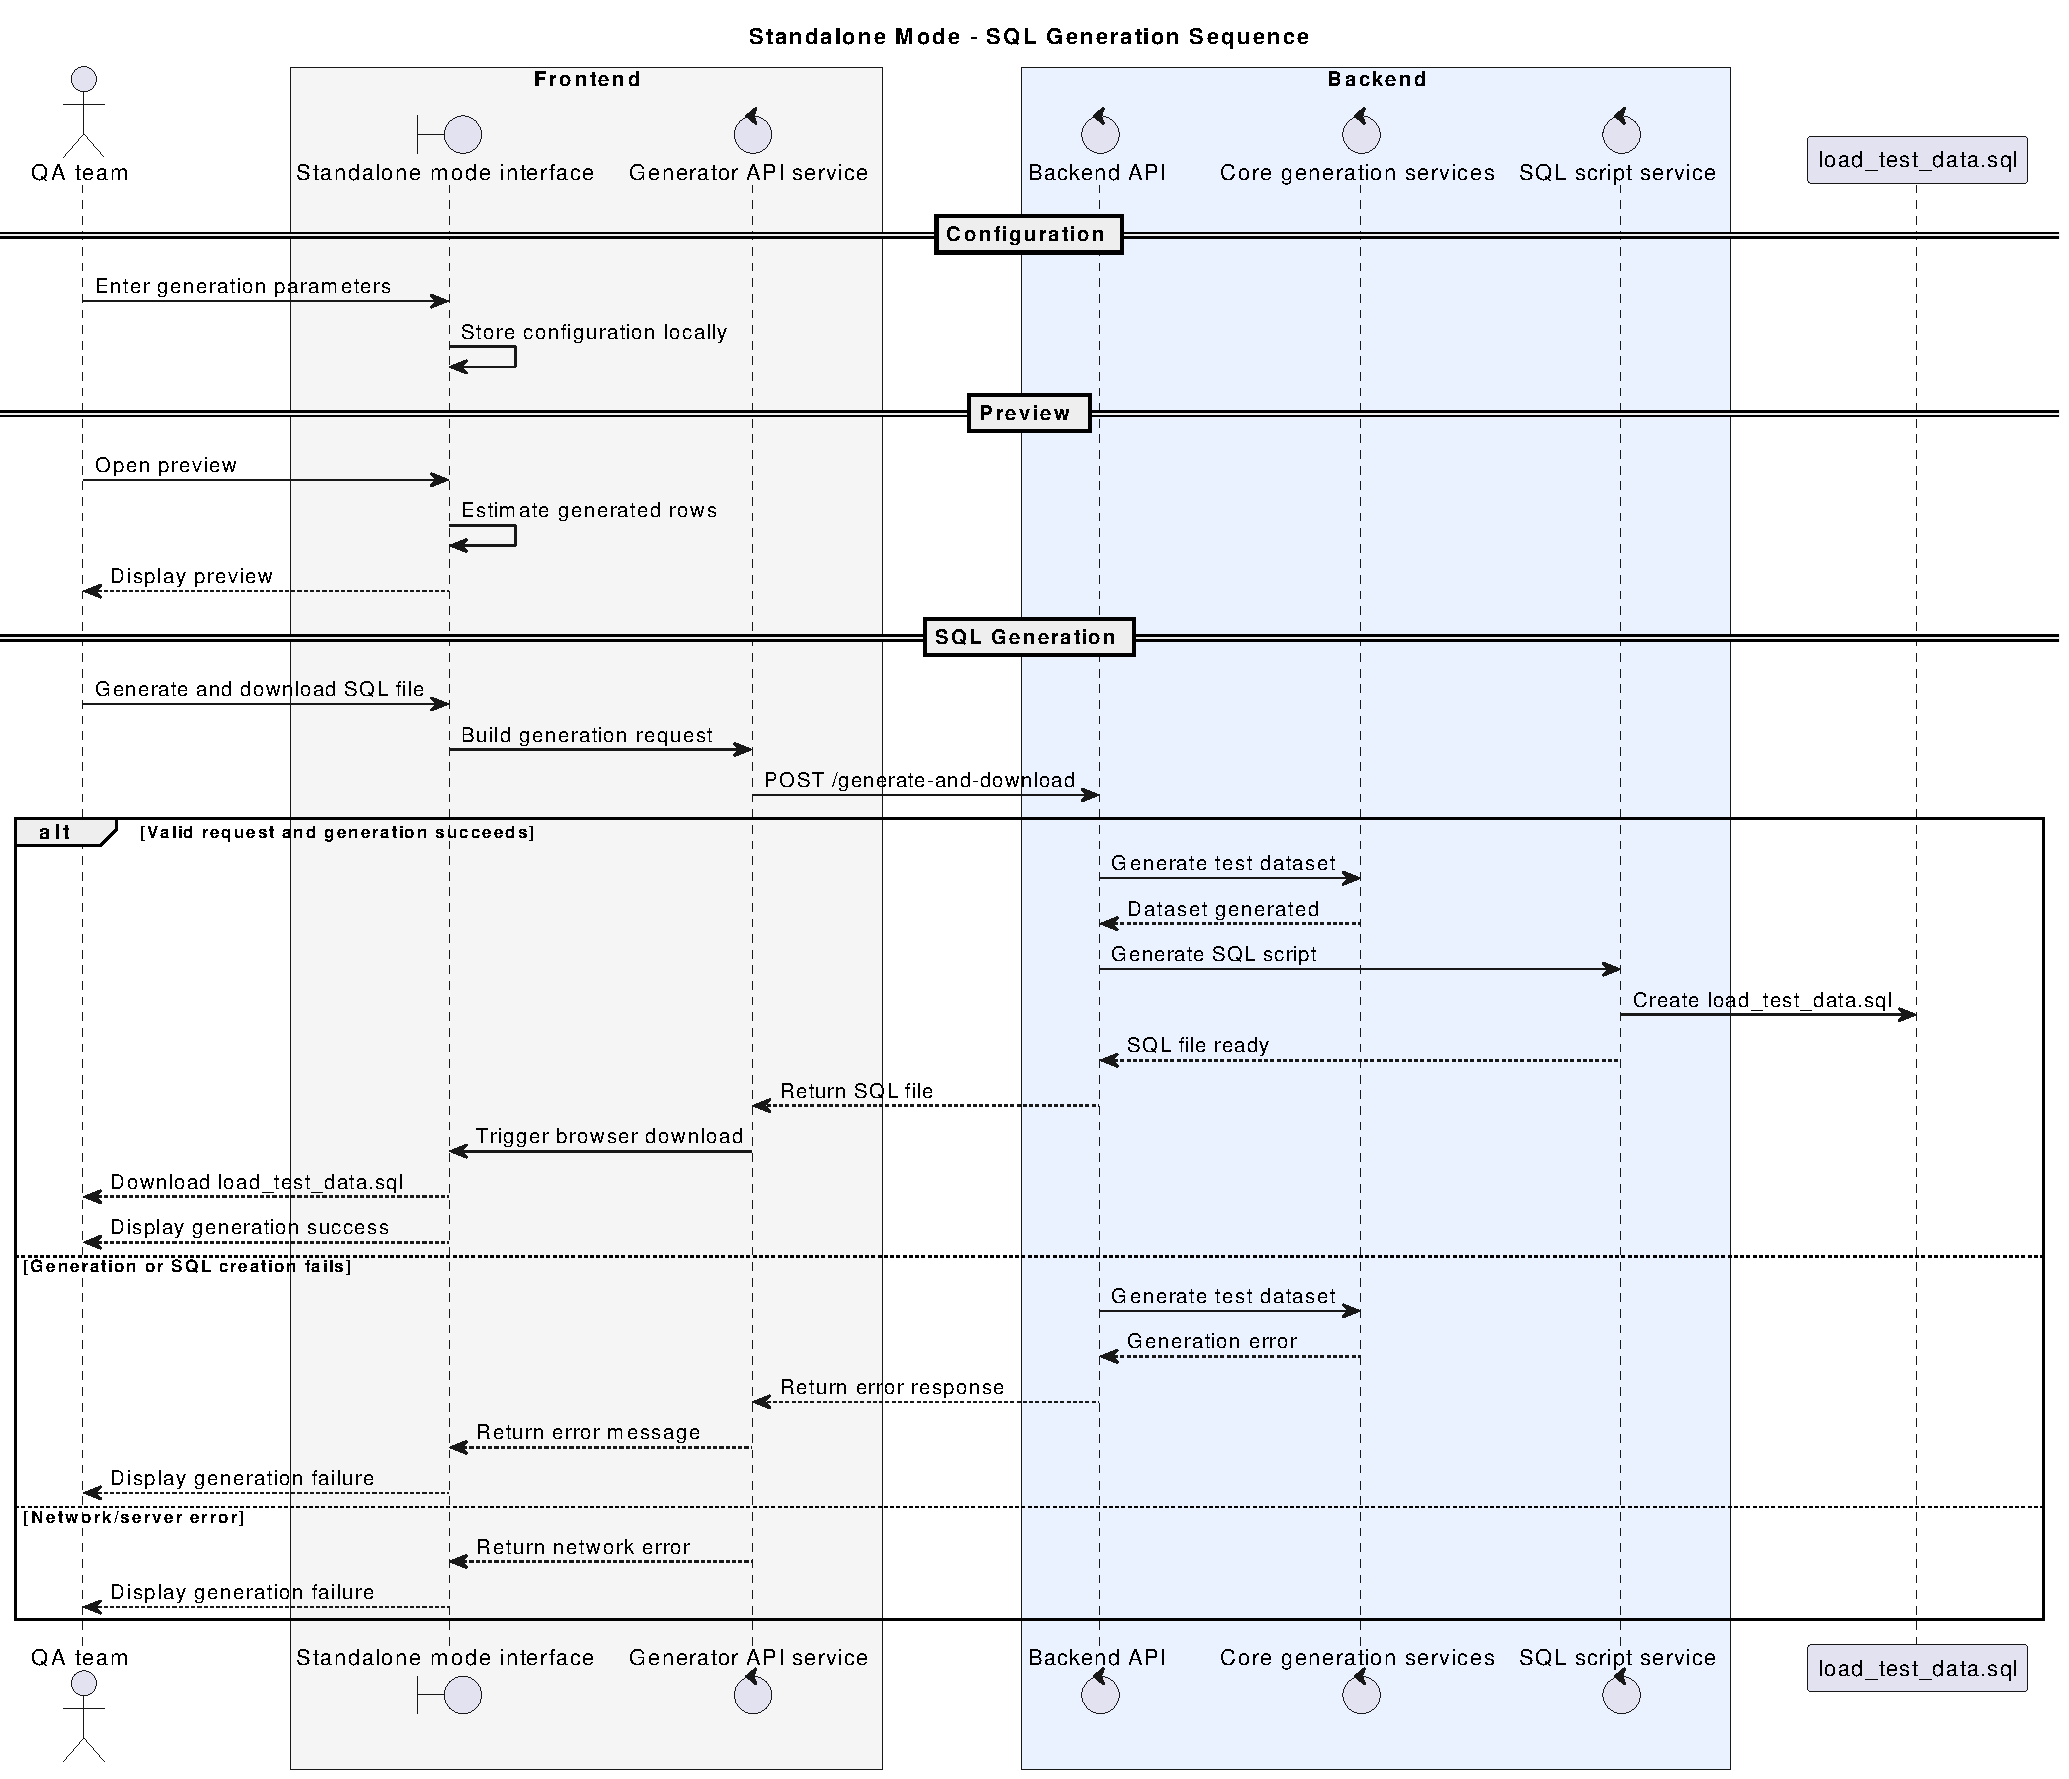
\includegraphics[width=0.95\textwidth]{img/sequence-standalone-mode.pdf}
\caption{Standalone mode SQL generation sequence}
\label{fig:sequence-standalone}
\end{figure}

\subsection{Backend Workflow Diagram}

\paragraph{}Figure~\ref{fig:ch4-backend-standalone-workflow} presents the backend workflow followed after
the QA engineer launches standalone generation.

\begin{figure}[!htbp]
\centering
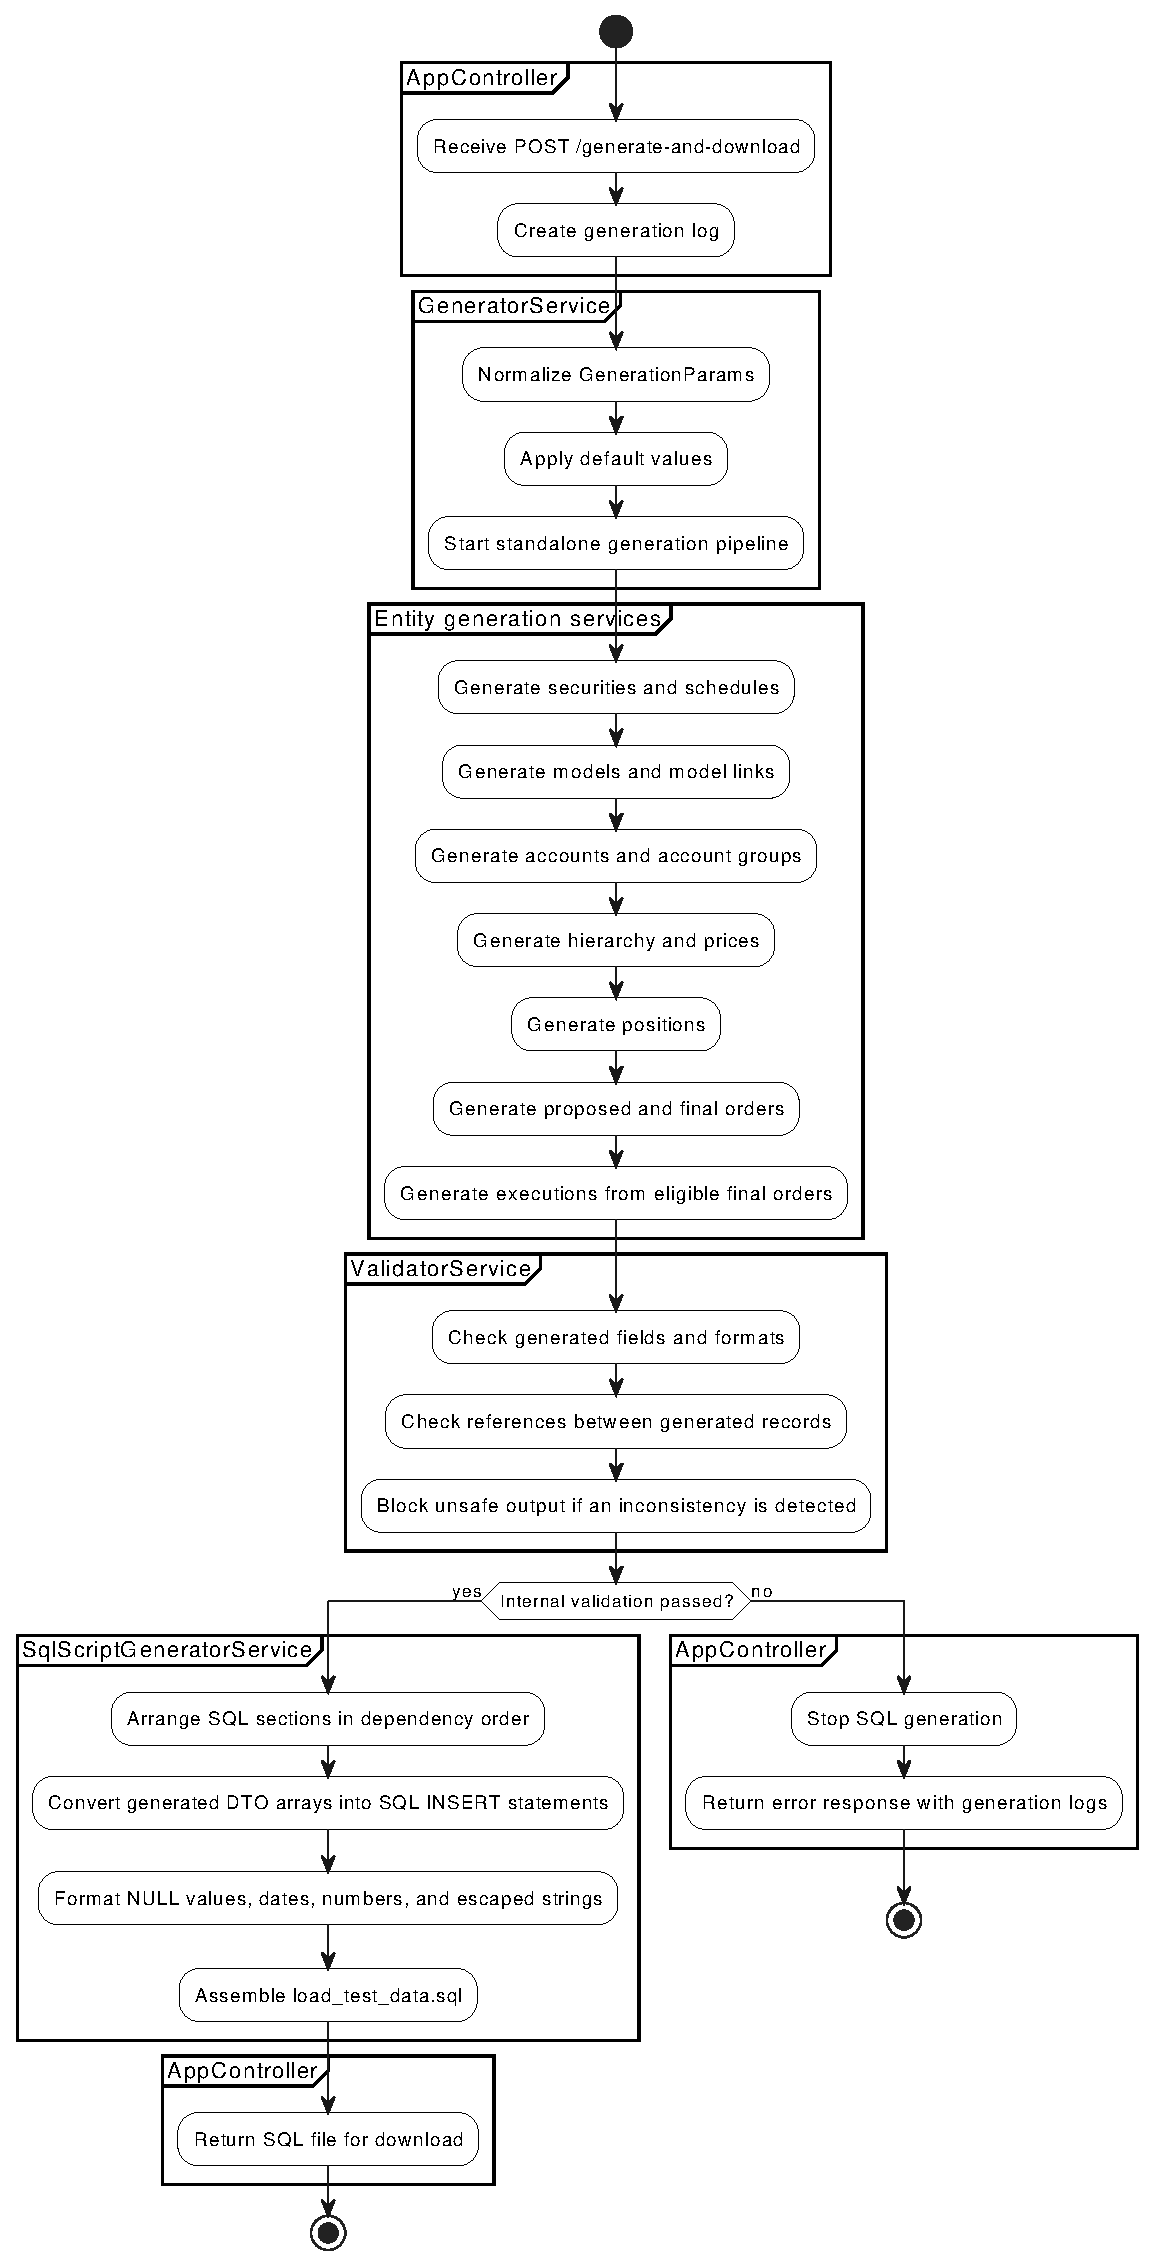
\includegraphics[width=0.95\textwidth,height=0.78\textheight,keepaspectratio]{img/ch4-backend-standalone-workflow.pdf}
\caption{Backend standalone SQL generation workflow}
\label{fig:ch4-backend-standalone-workflow}
\end{figure}

\section{Realization}

\subsection{Configuration Parameters}

\paragraph{}The standalone configuration page is implemented by \texttt{StandaloneConfigurationTab.tsx}
and shared configuration components. Table~\ref{tab:standalone-config-mapping} maps each section to
its main generation effect.

\renewcommand{\arraystretch}{1.12}
\begin{longtable}{|P{0.22\linewidth}|P{0.38\linewidth}|P{0.30\linewidth}|}
\caption{Standalone configuration mapping}
\label{tab:standalone-config-mapping} \\
\hline
\textbf{Section} & \textbf{Main inputs} & \textbf{Effect on generation} \\
\hline
\endfirsthead
\multicolumn{3}{r}{\tablename\ \thetable{} -- \textit{continued from previous page}} \\
\hline
\textbf{Section} & \textbf{Main inputs} & \textbf{Effect on generation} \\
\hline
\endhead
\hline
\multicolumn{3}{r}{\textit{continued on next page}} \\
\endfoot
\hline
\endlastfoot
Reference date & Base date selected from the date picker & Controls generated business dates such as prices, order dates, settlement dates, and execution dates. \\
\hline
Accounts & Enable flag, count (max: 5,000), currency, short name pattern, long name pattern & Creates the account universe used by dependent portfolio and trading data. \\
\hline
Securities & Enable flag and quantities for equity, fixed income, futures, options, FX forwards, and generic securities (max: 10,000 for equities, fixed income, and options; 5,000 for futures, FX forwards, and generics) & Creates the instrument universe used by prices, positions, orders, executions, and models. \\
\hline
Fixed-income schedules & CALL, PUT, COUP, and CONVERT rows per eligible fixed-income security (max: 20) & Adds optional schedule details for selected fixed-income instruments. \\
\hline
Proposed orders & Orders per account (max: 100), quantity range, buy/sell ratio & Creates proposed trade requests anchored to generated accounts and securities. \\
\hline
Final orders & Orders per account (max: 100), quantity range, buy/sell ratio & Creates order records that can be used by execution generation. \\
\hline
Positions & Positions per account (max: 100), long/short ratio, quantity range, value range, tax-lot option, tax lots per position (max: 10) & Creates account-security holdings and optional tax-lot splits. \\
\hline
Models & Models per account (max: 5), allocation mode, minimum allocation percentage & Creates model allocations using generated accounts and securities. \\
\hline
Executions & Executions per order (max: 5), partial fill percentage, commission rate type, commission rate & Creates fills for eligible generated orders. \\
\hline
\end{longtable}
\renewcommand{\arraystretch}{1}

\subsection{Preview Estimation}

\paragraph{}The preview is calculated on the frontend from the current configuration, without running
the backend generation algorithm. Table~\ref{tab:preview-estimation-rules} summarizes the main
estimation rules.

\renewcommand{\arraystretch}{1.15}
\begin{longtable}{|P{0.26\linewidth}|P{0.34\linewidth}|P{0.30\linewidth}|}
\caption{Preview estimation rules}
\label{tab:preview-estimation-rules} \\
\hline
\textbf{Estimated data} & \textbf{Formula or rule} & \textbf{Condition} \\
\hline
\endfirsthead
\multicolumn{3}{r}{\tablename\ \thetable{} -- \textit{continued from previous page}} \\
\hline
\textbf{Estimated data} & \textbf{Formula or rule} & \textbf{Condition} \\
\hline
\endhead
\hline
\multicolumn{3}{r}{\textit{continued on next page}} \\
\endfoot
\hline
\endlastfoot
Accounts & Account count & Account generation is enabled. \\
\hline
Securities & Sum of selected security subtype quantities & Security generation is enabled. \\
\hline
Prices & One price per generated security & At least one security is selected. \\
\hline
Positions & Accounts multiplied by positions per account, limited by available tradable securities & Positions are enabled and the configuration is valid. \\
\hline
Proposed orders & Accounts multiplied by proposed orders per account & Proposed orders are enabled and the configuration is valid. \\
\hline
Final orders & Accounts multiplied by orders per account & Orders are enabled and the configuration is valid. \\
\hline
Executions & Estimated equity orders multiplied by executions per order & Executions and orders are enabled. \\
\hline
Models & Accounts multiplied by models per account and allocation rows per model & Models are enabled and the configuration is valid. \\
\hline
\end{longtable}
\renewcommand{\arraystretch}{1}

\subsection{Internal Generation Algorithm}

\paragraph{}At this stage, the standalone data is generated by the application's internal algorithms.
The generated records are not taken from an existing database or from external input files. Instead,
the backend creates the requested accounts, securities, prices, positions, orders, executions, and
related records from the configuration entered by the QA engineer. It relies on predefined templates
and code lists stored in the backend, then applies controlled pseudo-random variation to generate
different names, quantities, prices, dates, and trading values while preserving the required links
between records.


\subsection{User Workflow}

\paragraph{}The following figures show the implemented standalone screens. Their routing and state
transitions are managed by \texttt{StandaloneMode.tsx}.

\paragraph{}Figure~\ref{fig:ch4-mode-selection} shows the entry screen where the user selects the
standalone mode.

\begin{figure}[!htbp]
\centering
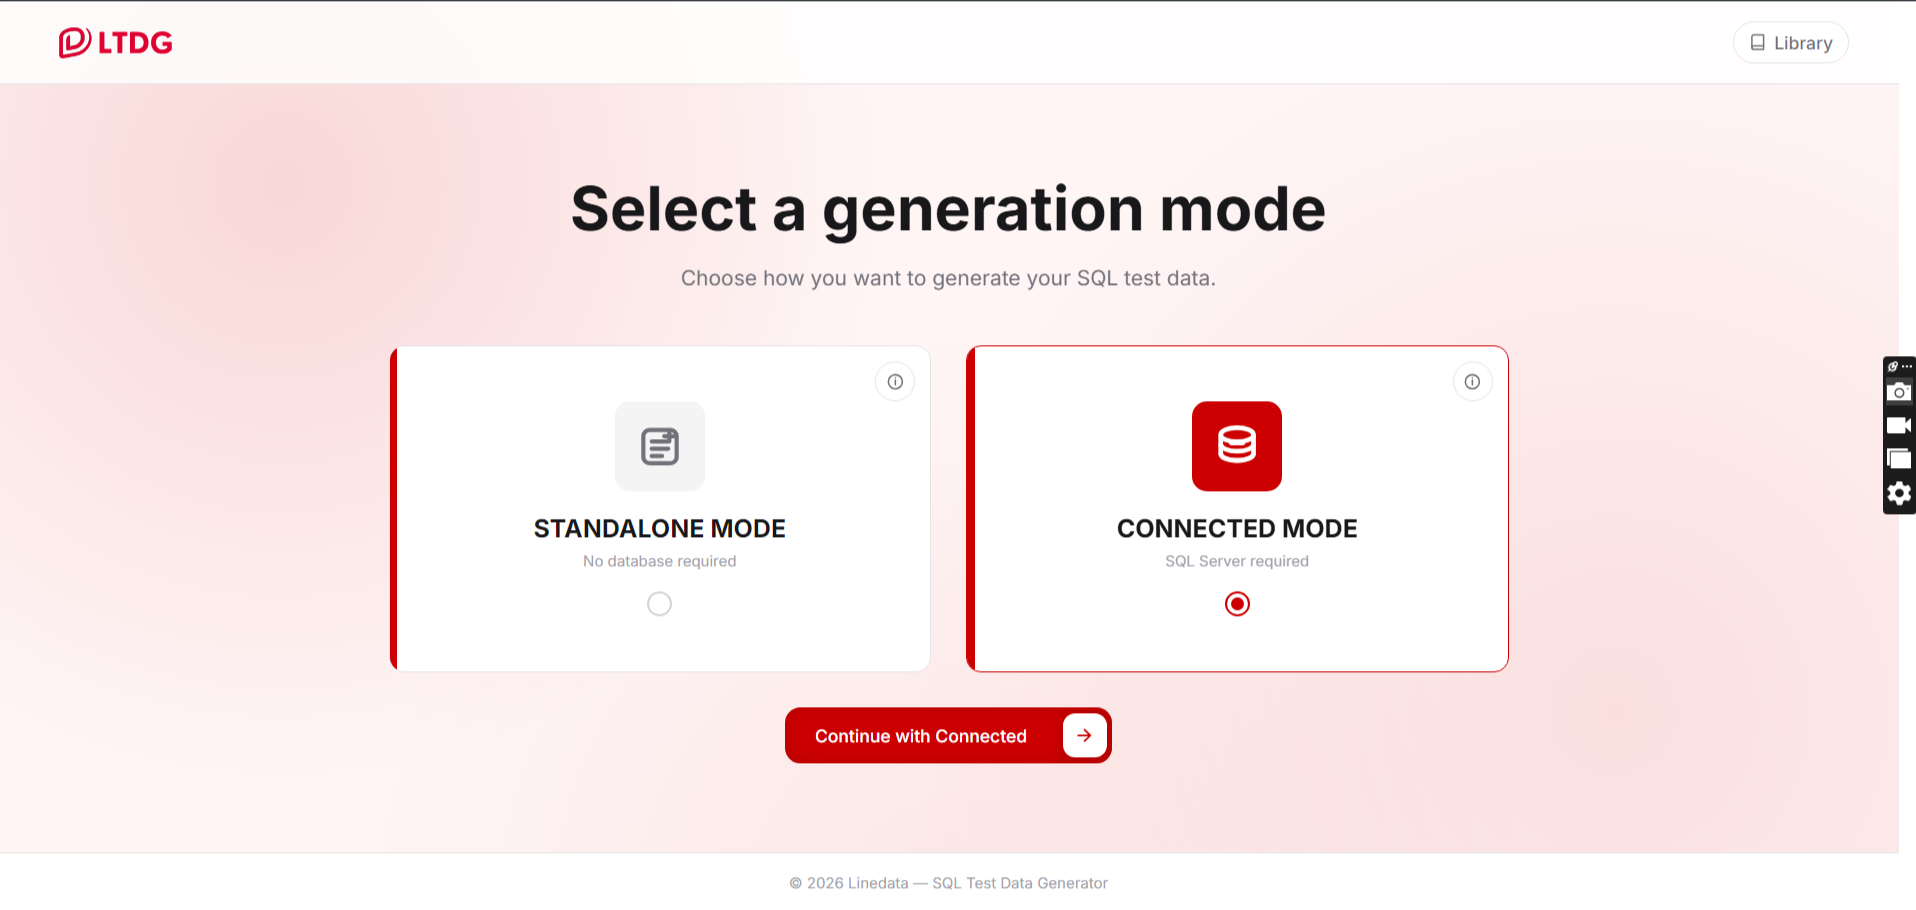
\includegraphics[width=0.88\textwidth]{img/ch4-mode-selection.png}
\caption{Mode selection screen}
\label{fig:ch4-mode-selection}
\end{figure}

\paragraph{}Figure~\ref{fig:ch4-step-config} shows the configuration screen where the QA engineer
defines the generation scope and the main parameters used by the backend.

\begin{figure}[!htbp]
\centering
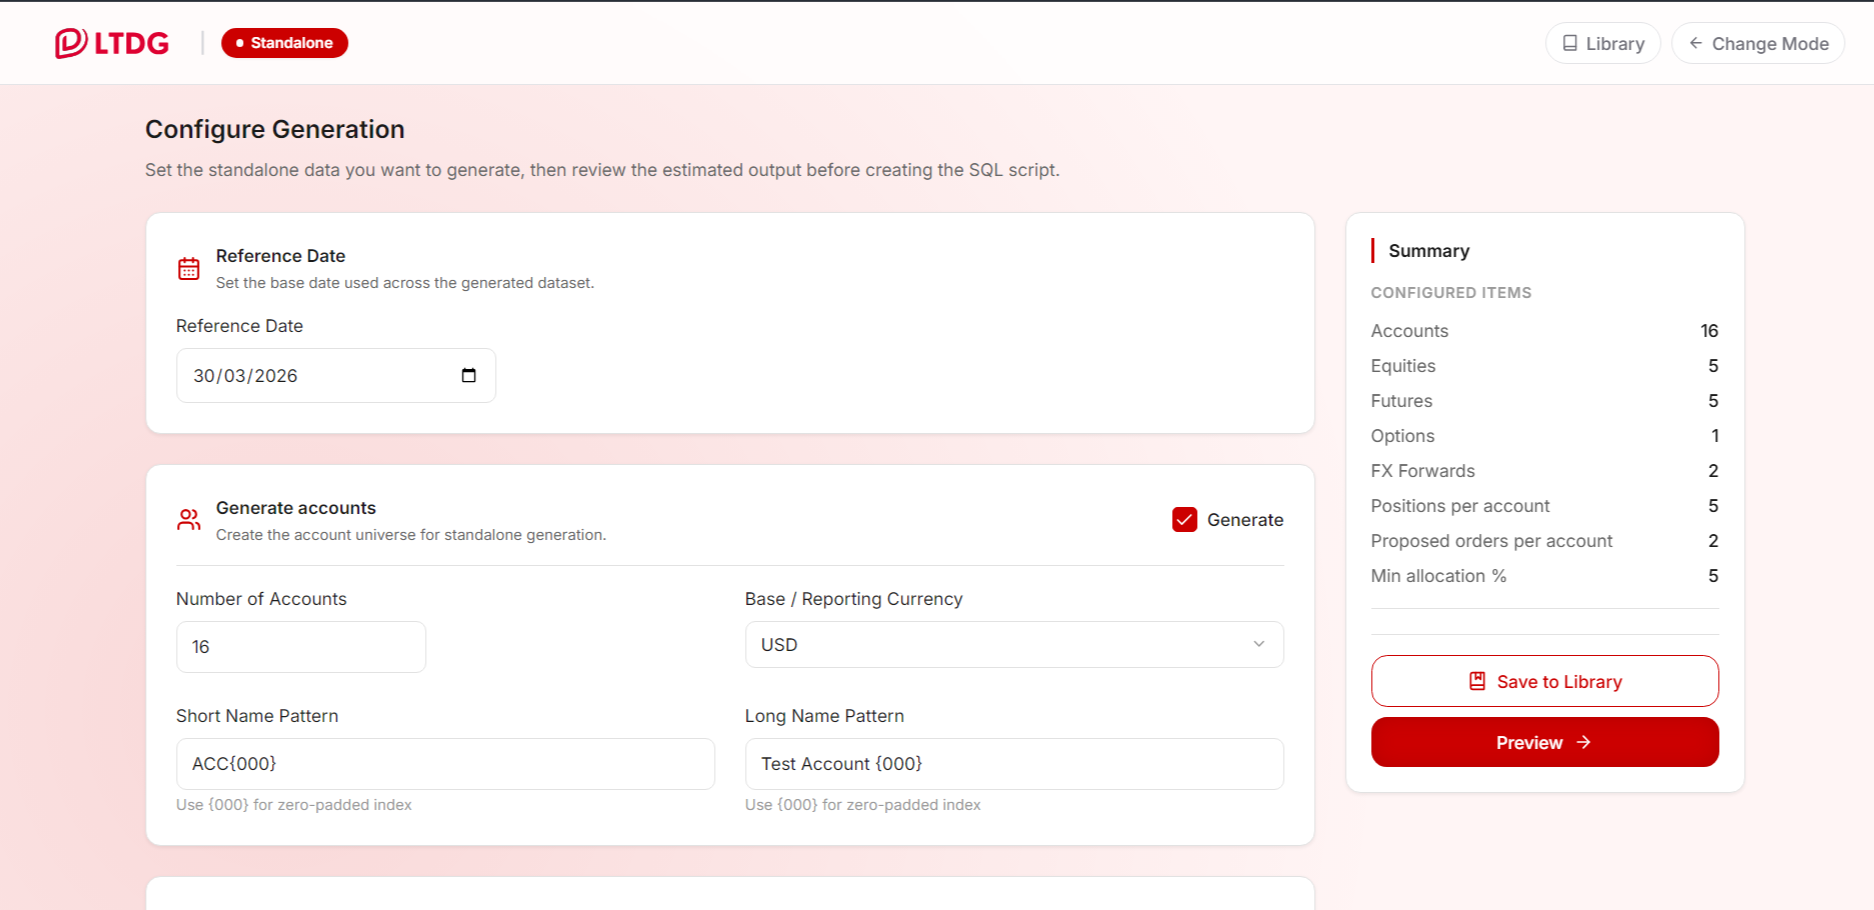
\includegraphics[width=0.88\textwidth]{img/ch4-step1-config.png}
\caption{Standalone configuration screen}
\label{fig:ch4-step-config}
\end{figure}

\paragraph{}Figure~\ref{fig:ch4-step-preview} shows the preview screen that summarizes the expected
result before the SQL generation request is launched.

\begin{figure}[!htbp]
\centering
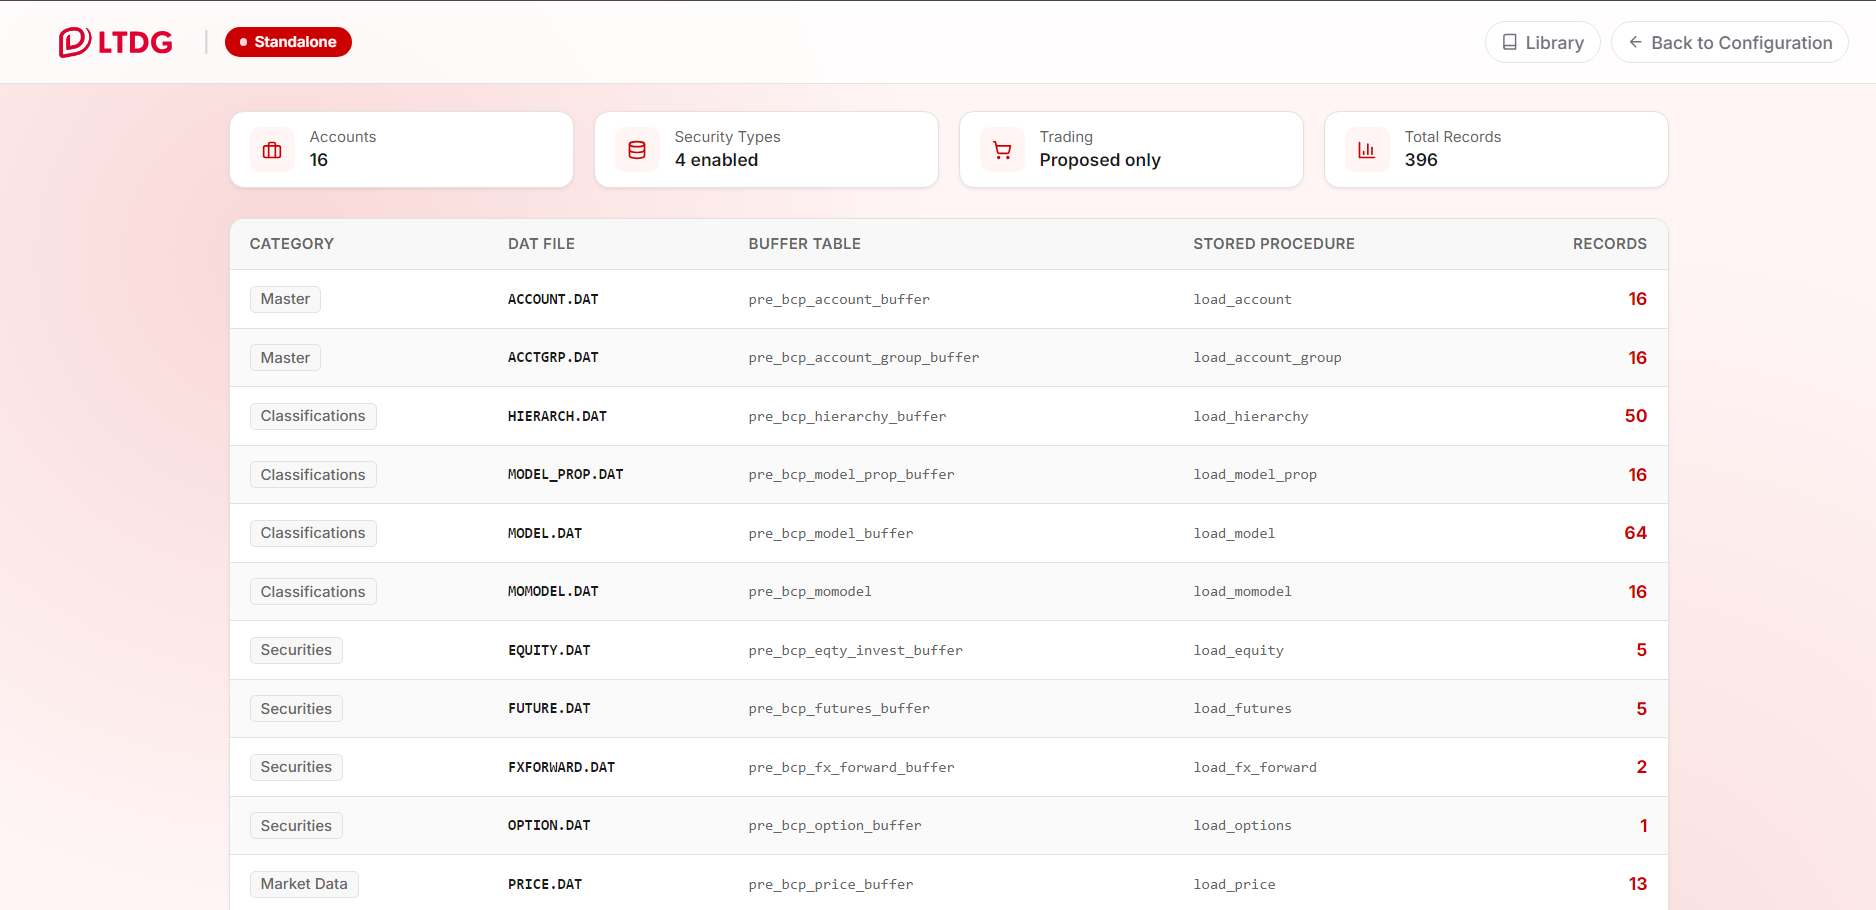
\includegraphics[width=0.88\textwidth]{img/ch4-step2-preview.png}
\caption{Standalone preview screen}
\label{fig:ch4-step-preview}
\end{figure}

\paragraph{}Figure~\ref{fig:ch4-step-result} shows the result screen displayed after generation, with
the execution status and access to the generated SQL script.

\begin{figure}[!htbp]
\centering
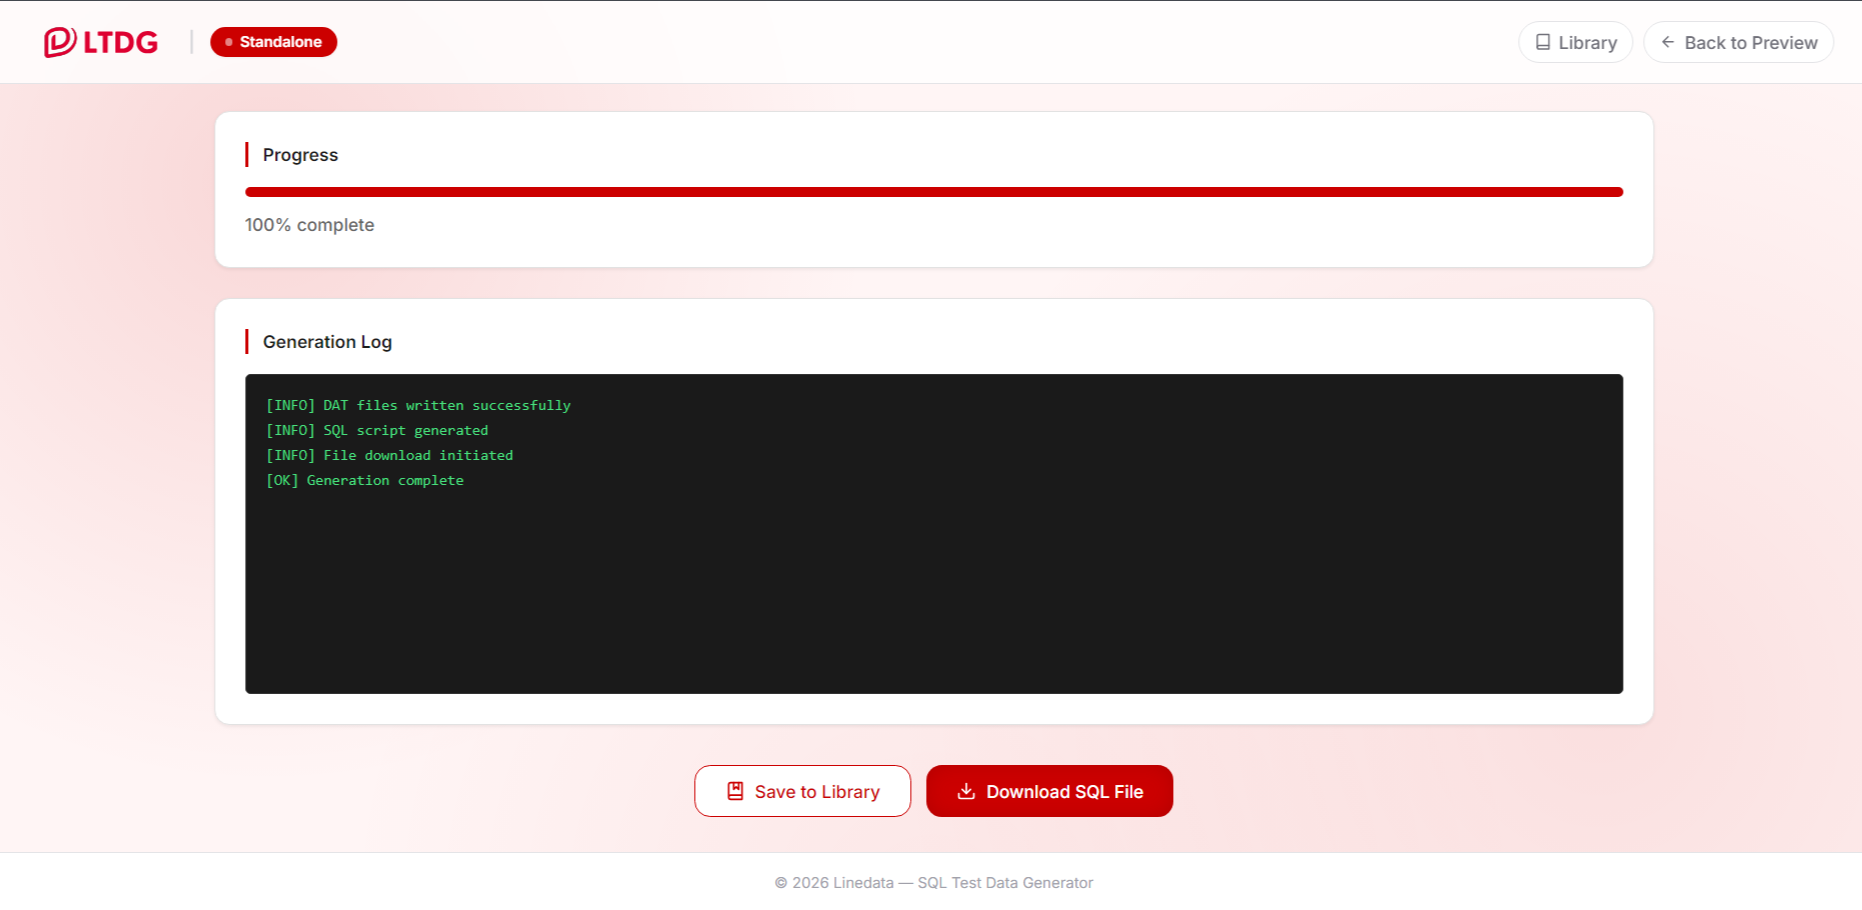
\includegraphics[width=0.88\textwidth]{img/ch4-step3-result.png}
\caption{Standalone generation result}
\label{fig:ch4-step-result}
\end{figure}

\subsection{Generated Output Evidence}

\paragraph{}After the QA engineer launches generation, the backend produces the configured
\texttt{.DAT} files, validates their field formats and relationships, and converts the validated output
into a SQL Server loading script. Table~\ref{tab:standalone-realization-proof} summarizes the main
realization evidence of this sprint.

\Needspace{12\baselineskip}
\renewcommand{\arraystretch}{1.3}
\begin{longtable}{|P{0.25\linewidth}|P{0.35\linewidth}|P{0.30\linewidth}|}
\caption{Standalone generation realization evidence}
\label{tab:standalone-realization-proof} \\
\hline
\textbf{Evidence} & \textbf{Implemented result} & \textbf{Purpose} \\
\hline
\endfirsthead
\multicolumn{3}{r}{\tablename\ \thetable{} -- \textit{continued from previous page}} \\
\hline
\textbf{Evidence} & \textbf{Implemented result} & \textbf{Purpose} \\
\hline
\endhead
\hline
\multicolumn{3}{r}{\textit{continued on next page}} \\
\endfoot
\hline
\endlastfoot
Generated files & The backend writes files such as \texttt{ACCOUNT.DAT}, \texttt{EQUITY.DAT}, \texttt{PRICE.DAT}, \texttt{POSITION.DAT}, \texttt{ORDER.DAT}, and \texttt{EXECUTION.DAT}. & Proves that the configuration is transformed into concrete Longview loading artifacts. \\
\hline
Field validation & Each generated file is checked against required fields, numeric fields, date formats, lengths, and flag values. & Prevents malformed rows from being exported. \\
\hline
Relationship validation & Accounts, securities, prices, positions, orders, executions, and models are checked before writing the final output. & Ensures that generated records reference existing generated entities. \\
\hline
SQL script generation & The validated \texttt{.DAT} files are converted into \texttt{load\_test\_data.sql}. & Provides a single SQL Server script that can be downloaded and executed by the QA engineer. \\
\hline
Generation feedback & The interface displays progress, warning, success, and error messages during the run. & Gives the user visibility over the generation process and its result. \\
\hline
\end{longtable}
\renewcommand{\arraystretch}{1}

\paragraph{}Figure~\ref{fig:ch4-generation-proof} can be completed later with a screenshot of the
generation log, the produced \texttt{.DAT} files, or a short excerpt from the generated SQL script.

\begin{figure}[!htbp]
\centering
\IfFileExists{img/ch4-generation-proof.png}{%
    \includegraphics[width=0.88\textwidth]{img/ch4-generation-proof.png}%
}{%
    \fbox{\parbox[c][0.22\textheight][c]{0.86\textwidth}{\centering Screenshot to be added: standalone generation log, generated DAT files, or SQL script excerpt}}%
}
\caption{Standalone generation output and validation evidence}
\label{fig:ch4-generation-proof}
\end{figure}

\section*{Conclusion}
\addcontentsline{toc}{section}{Conclusion}

\paragraph{}Sprint 2 delivered the first complete version of the test data generator through standalone
configuration, preview, generation, validation, and SQL export. This result prepares the transition
to the connected mode introduced in the next sprint.

        \clearpage
        
        \chapter{Sprint 3 -- Connected Mode and SQL Server Integration}


% ─────────────────────────────────────────────
\section*{Introduction}
\addcontentsline{toc}{section}{Introduction}
% ─────────────────────────────────────────────


\paragraph{}This chapter presents Sprint 3, which spanned four weeks and extended the generator from a standalone synthetic tool
into a connected assistant capable of working with an existing Longview SQL Server environment.
The objective of this sprint was to allow QA engineers to connect to a database, browse selected
reference entities, choose the subset of data to reuse, and generate additional pre-BCP records
anchored to that database state. This mode preserves the same output objective as standalone mode:
a coherent SQL loading script, but it builds part of the dataset from existing accounts or securities
instead of generating everything from scratch.

\paragraph{}The sprint therefore focused on three major concerns: secure database access, selective data
grabbing, and connected generation. The implementation introduced a dedicated
\texttt{DatabaseModule}, a \texttt{ConnectedController}, a \texttt{DatabaseService} for SQL Server
connectivity, and a \texttt{ConnectedGeneratorService} that reuses the entity generation services
implemented in Sprint 2 while adapting them to grabbed database records.

\paragraph{}The chapter follows the same sprint structure as the previous implementation chapter:
sprint backlog, sprint specification, sprint design, implementation, sprint review and validation,
then conclusion. To avoid repetition, it focuses only on what connected mode adds to the
standalone generation engine.


% ─────────────────────────────────────────────
\section{Sprint Backlog}
% ─────────────────────────────────────────────


\paragraph{}Sprint 3 targeted the connected-mode user story from the product backlog: connecting to a
Longview SQL Server instance in read-only mode and generating coherent records from existing
reference data. The sprint backlog is presented in Table~\ref{tab:sprint3-backlog}.

\renewcommand{\arraystretch}{1.35}
\begin{longtable}{|Q{0.06\linewidth}|P{0.30\linewidth}|P{0.42\linewidth}|Q{0.12\linewidth}|}
\caption{Sprint 3 backlog}
\label{tab:sprint3-backlog} \\
\hline
\textbf{ID} & \textbf{Task} & \textbf{Description} & \textbf{Estimate} \\
\hline
\endfirsthead
\multicolumn{4}{r}{\tablename\ \thetable{} -- \textit{continued from previous page}} \\
\hline
\textbf{ID} & \textbf{Task} & \textbf{Description} & \textbf{Estimate} \\
\hline
\endhead
\hline
\multicolumn{4}{r}{\textit{continued on next page}} \\
\endfoot
\hline
\endlastfoot
T3-1 & Implement SQL Server connection service & Create a service able to test, open, reuse, and close SQL Server connections using either Windows authentication or SQL authentication. & 2 days \\
\hline
T3-2 & Implement connected backend API & Add endpoints for testing the connection, connecting, disconnecting, fetching allowed tables, grabbing account groups, grabbing accounts, previewing generation, and generating the final SQL script. & 2 days \\
\hline
T3-3 & Implement data grabbing logic & Allow users to select existing account groups, accounts, and securities, then transform database rows into DTO-compatible records for the generation pipeline. & 2 days \\
\hline
T3-4 & Implement connected generation service & Build a connected orchestrator that combines grabbed records with newly generated dependent records such as prices, positions, orders, models, and executions. & 2 days \\
\hline
T3-5 & Implement connected frontend workflow & Build the connection, data grabber, configuration, preview, and generation steps under the \texttt{/connected} route. & 2 days \\
\hline
T3-6 & Add safeguards and validation & Restrict raw table fetching to approved tables, require a live connection before connected actions, and validate generated output before writing files. & 1 day \\
\hline
\end{longtable}


% ─────────────────────────────────────────────
\section{Sprint Specification}
\paragraph{}Connected mode extends the standalone generation use case by adding a database preparation
phase. Before generation, the QA engineer connects to SQL Server and selects existing accounts or
securities that will serve as anchors for the generated scenario.

\renewcommand{\arraystretch}{1.15}
\begin{longtable}{|P{0.24\linewidth}|P{0.66\linewidth}|}
\caption{Textual description of the connected generation use case}
\label{tab:connected-usecase-description} \\
\hline
\textbf{Element} & \textbf{Description} \\
\hline
\endfirsthead
\multicolumn{2}{r}{\tablename\ \thetable{} -- \textit{continued from previous page}} \\
\hline
\textbf{Element} & \textbf{Description} \\
\hline
\endhead
\hline
\multicolumn{2}{r}{\textit{continued on next page}} \\
\endfoot
\hline
\endlastfoot
Use case & Generate a SQL loading script anchored to existing Longview data. \\
\hline
Actor & QA Engineer. \\
\hline
Preconditions & A SQL Server instance is reachable and the QA engineer has valid read-only connection information. \\
\hline
Postconditions & Existing records are reused as anchors and a coherent \texttt{load\_test\_data.sql} file is generated. \\
\hline
Nominal scenario &
\begin{enumerate}[leftmargin=*,nosep]
    \item The QA engineer enters SQL Server connection information.
    \item The system tests and opens the connection.
    \item The QA engineer grabs existing accounts, account groups, or securities.
    \item The system infers the connected generation case from the selected data.
    \item The QA engineer configures only the missing or dependent records.
    \item The system previews the result, then generates the final SQL script.
\end{enumerate} \\
\hline
Exception scenario &
\begin{itemize}[leftmargin=*,nosep]
    \item If connection fails, the workflow stops before data grabbing.
    \item If no compatible data is selected, preview and generation are rejected.
    \item If a selected table is not allowed, the backend refuses the request.
\end{itemize} \\
\hline
\end{longtable}


\section{Sprint Design}
% ─────────────────────────────────────────────


\subsection{Connected Mode Use Case Diagram}

\paragraph{}Figure~\ref{fig:usecase-connected} presents the connected mode use cases implemented in this
sprint. This mode adds database-specific actions such as testing the connection, connecting with
Windows authentication or SQL Server authentication, grabbing account and security reference data,
and disconnecting from SQL Server. The SQL Server actor is involved only through read-only
operations.

\begin{figure}[H]
\centering
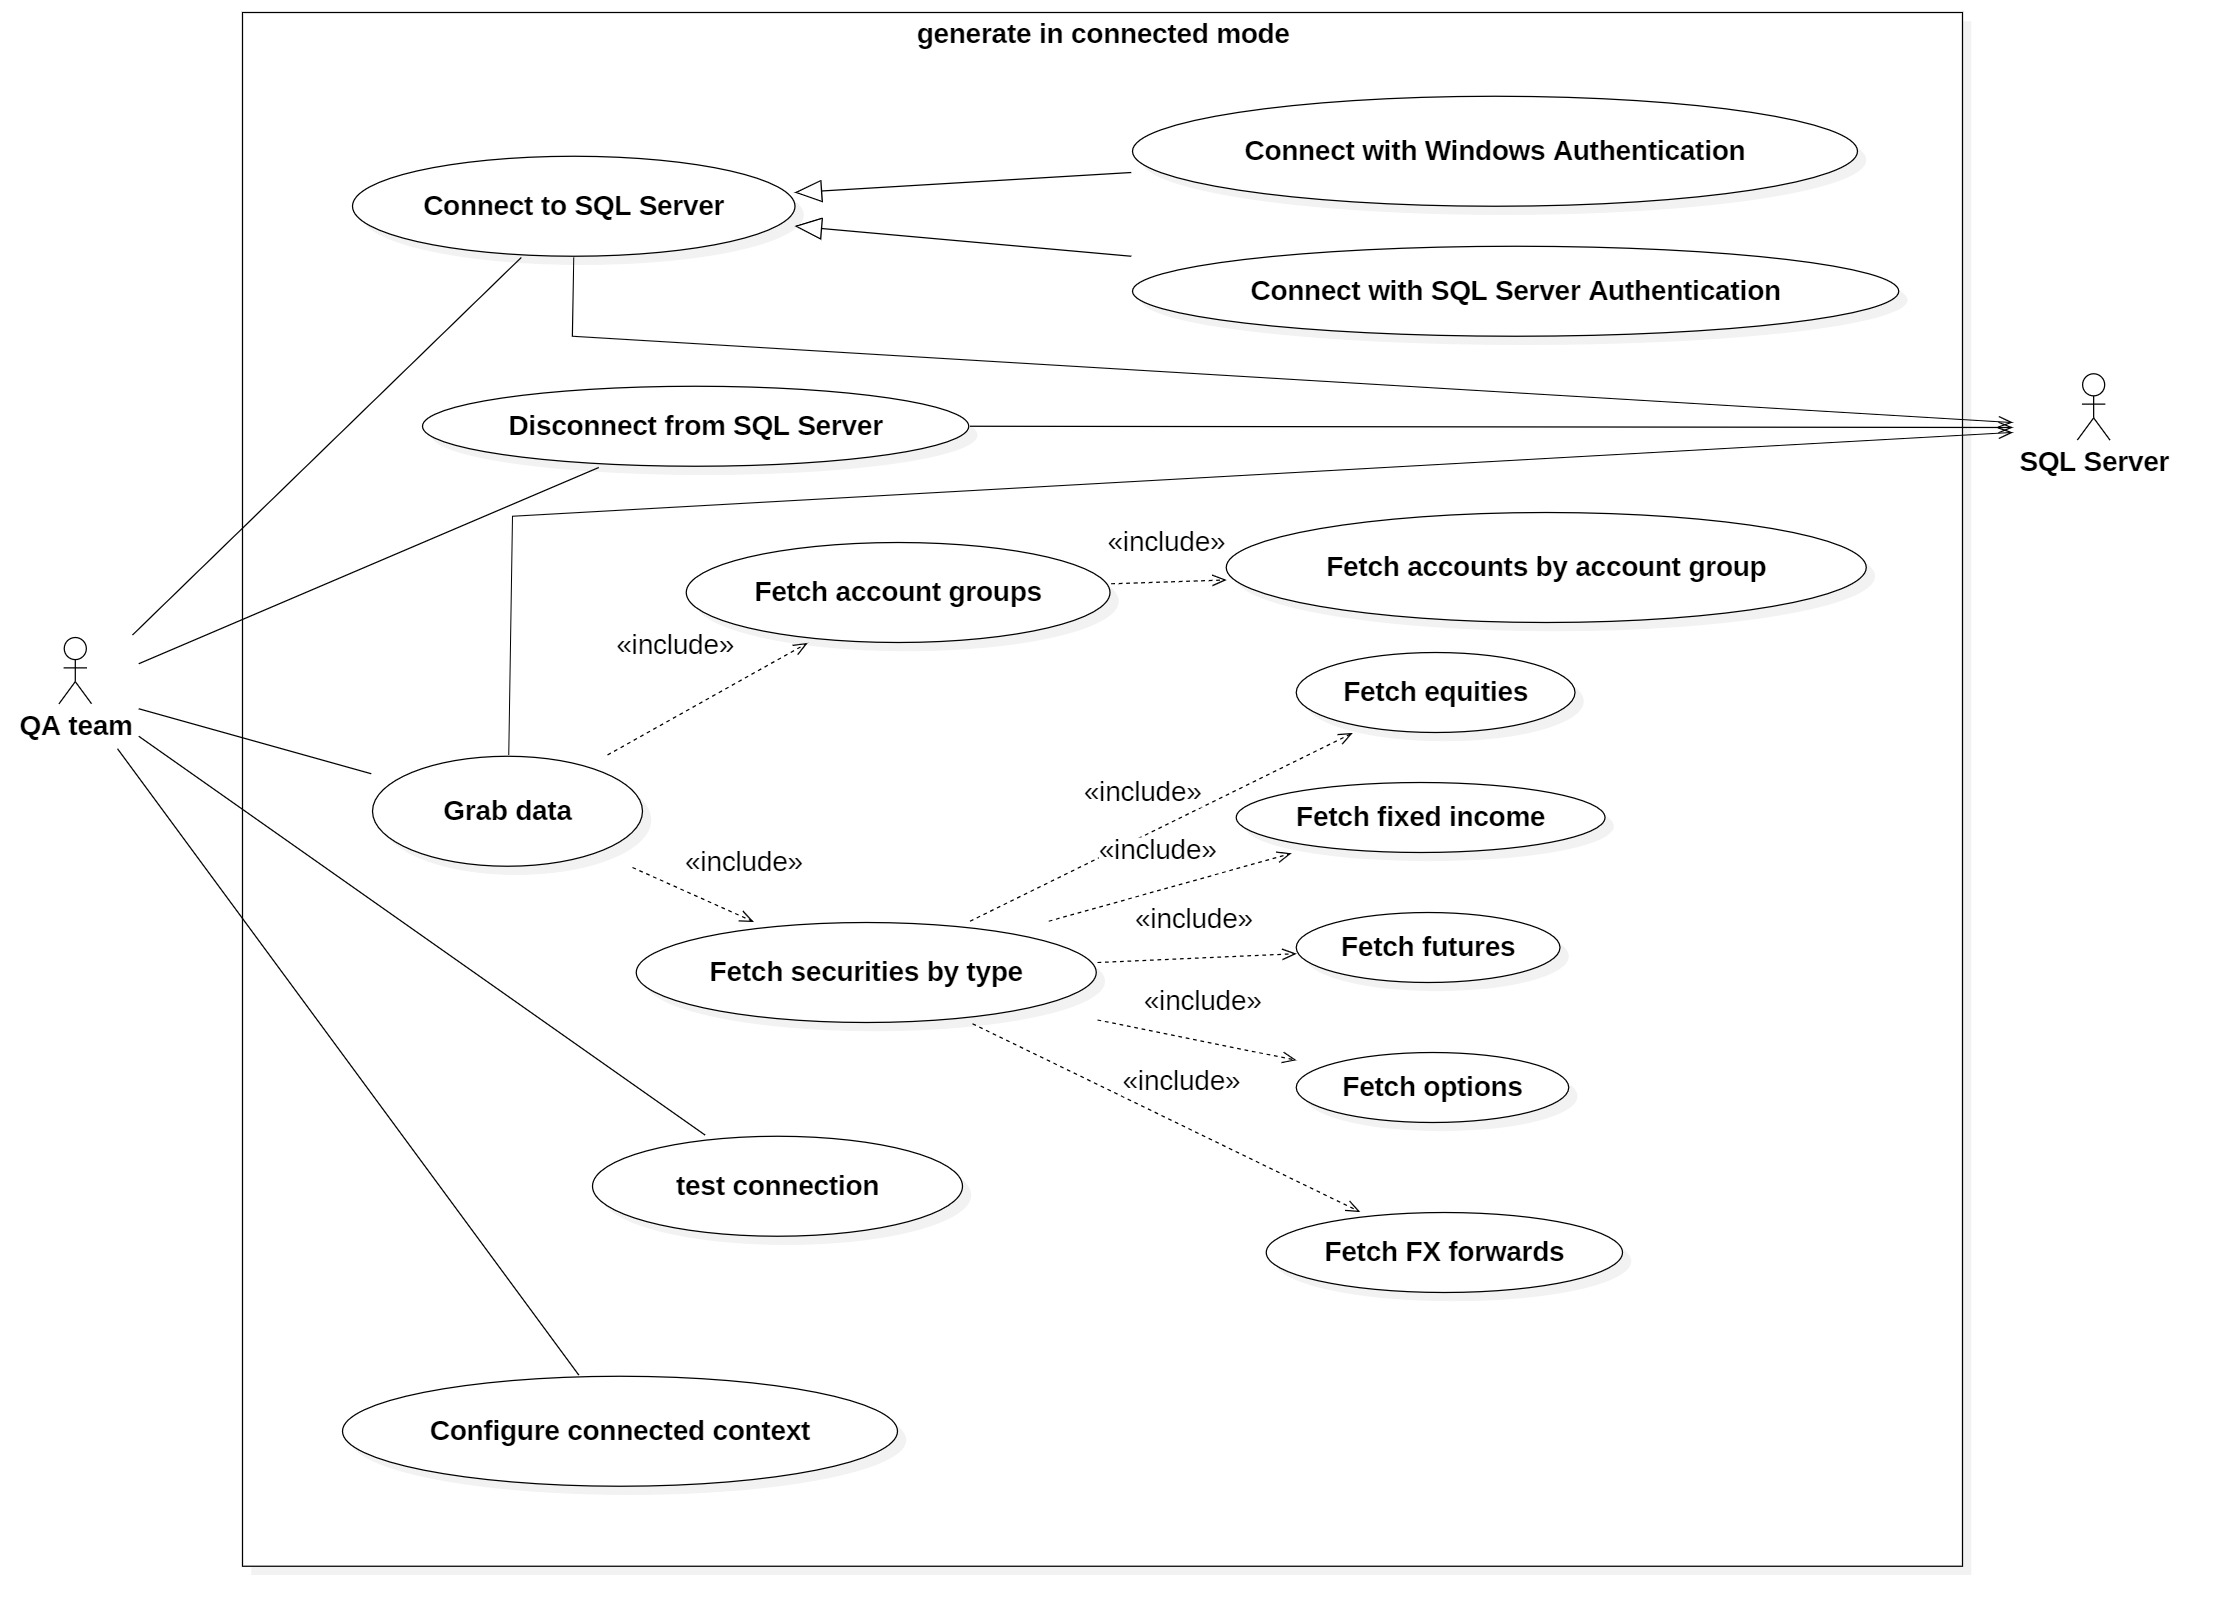
\includegraphics[width=1\textwidth]{img/usecase-connected-mode.jpg}
\caption{Connected mode use case diagram}
\label{fig:usecase-connected}
\end{figure}

\subsection{Connected Mode Architecture}

\paragraph{}Connected mode is built as an extension of the generation engine rather than as a separate
generator. The backend introduces the \texttt{DatabaseModule}, which groups the
\texttt{ConnectedController}, the \texttt{DatabaseService}, and the
\texttt{ConnectedGeneratorService}. The \texttt{DatabaseService} owns the SQL Server connection pool,
while the connected generator receives grabbed data, prepares the connected dataset, validates it,
and delegates SQL script assembly to the same \texttt{SqlScriptGeneratorService} used by standalone
mode.

\paragraph{}This architecture avoids duplication: connected mode reuses the account, account group,
hierarchy, security, price, model, position, order, execution, validator, and SQL script services
implemented during Sprint 2. The connected-specific layer is responsible only for selecting the
source data, mapping database rows to generator DTOs, and deciding which dependent records must be
generated according to the selected grab mode.

\begin{figure}[htbp]
\centering
%\includegraphics[width=1\textwidth]{img/ch5-connected-architecture.pdf}
\caption{Architecture of the connected mode}
\label{fig:ch5-connected-architecture}
\end{figure}

\subsection{Connected Workflow}

\paragraph{}The frontend implements connected mode as a five-step workflow:
\texttt{/connected/connection}, \texttt{/connected/data-grabber},
\texttt{/connected/configuration}, \texttt{/connected/preview}, and
\texttt{/connected/generation}. This sequence reflects the additional constraints introduced by
database usage: the user must connect first, then grab reference data, then configure only the
records that still need to be generated.

\renewcommand{\arraystretch}{1.3}
\begin{longtable}{|P{0.18\linewidth}|P{0.28\linewidth}|P{0.44\linewidth}|}
\caption{Connected mode workflow}
\label{tab:connected-workflow} \\
\hline
\textbf{Step} & \textbf{Route} & \textbf{Purpose} \\
\hline
\endfirsthead
\multicolumn{3}{r}{\tablename\ \thetable{} -- \textit{continued from previous page}} \\
\hline
\textbf{Step} & \textbf{Route} & \textbf{Purpose} \\
\hline
\endhead
\hline
\multicolumn{3}{r}{\textit{continued on next page}} \\
\endfoot
\hline
\endlastfoot
Connection & \texttt{/connected/connection} & Enter SQL Server details, choose authentication mode, test the connection, and open the active backend connection. \\
\hline
Data grabber & \texttt{/connected/data-grabber} & Browse available account groups, accounts, and security buffer tables, then select the records that will anchor generation. \\
\hline
Configuration & \texttt{/connected/configuration} & Configure generated complements such as accounts, securities, prices, models, positions, orders, and executions. \\
\hline
Preview & \texttt{/connected/preview} & Run the backend generation rules without writing files and display estimated rows, summaries, warnings, and samples. \\
\hline
Generation & \texttt{/connected/generation} & Generate the connected dataset, assemble the SQL script, and download \texttt{load\_test\_data.sql}. \\
\hline
\end{longtable}

\begin{figure}[htbp]
\centering
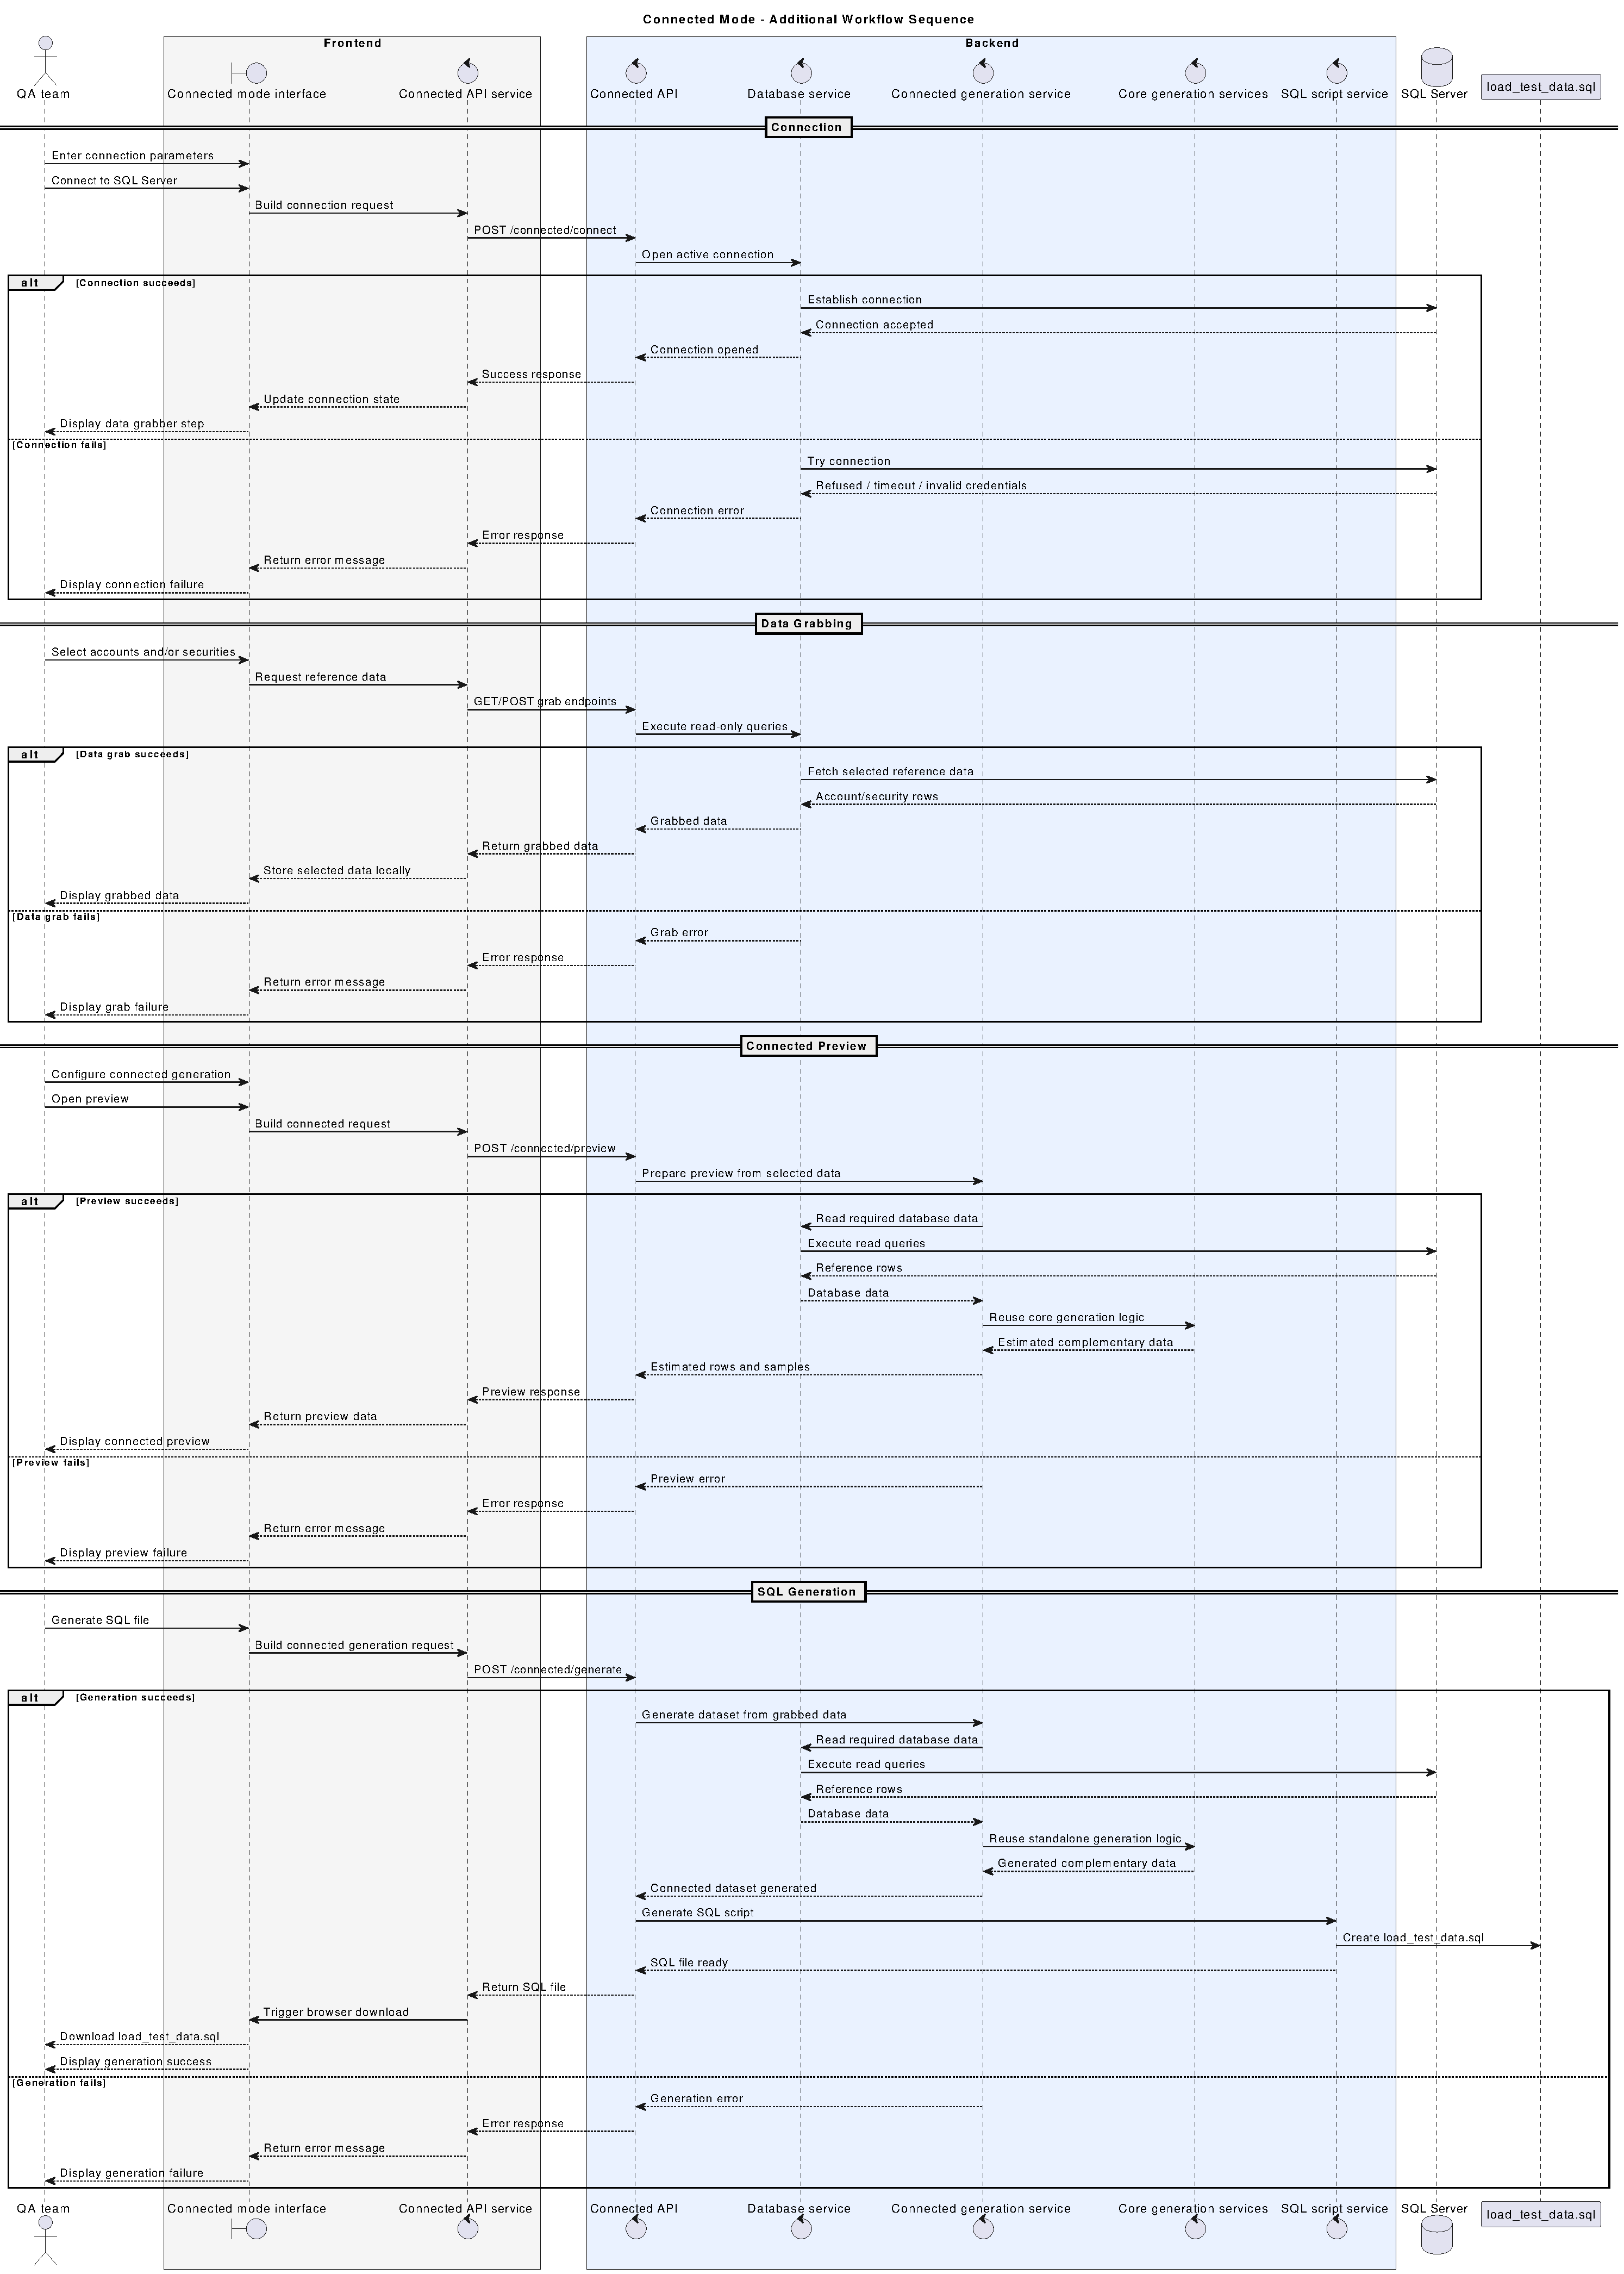
\includegraphics[width=1\textwidth]{img/sequence-connected-mode.pdf}
\caption{Connected mode workflow sequence}
\label{fig:ch5-connected-sequence}
\end{figure}

\paragraph{}Figure~\ref{fig:ch5-connected-sequence} details the additional exchanges introduced by
connected mode. Compared with standalone generation, the workflow begins with a SQL Server
connection request, continues with read-only data grabbing, and only then reaches preview and SQL
generation. The connected API delegates database access to \texttt{DatabaseService}, while
\texttt{ConnectedGeneratorService} prepares the selected account and security context before reusing
the core generation services.

\paragraph{}The alternate branches in the sequence diagram show how the application handles connection
errors, failed data grabs, preview errors, and generation failures. These paths are important
because connected mode depends on external database availability; every backend failure is returned
as a structured frontend message instead of leaving the user in an ambiguous state.

\subsection{Grab Modes}

\paragraph{}Connected generation supports three cases, referred to in the implementation as
\texttt{grabMode}. The grab mode is inferred automatically on the frontend from the selected data
and is sent to the backend as part of the connected generation request.

\renewcommand{\arraystretch}{1.3}
\begin{longtable}{|P{0.24\linewidth}|P{0.32\linewidth}|P{0.34\linewidth}|}
\caption{Connected generation grab modes}
\label{tab:grab-modes} \\
\hline
\textbf{Grab mode} & \textbf{Grabbed data} & \textbf{Generated complement} \\
\hline
\endfirsthead
\multicolumn{3}{r}{\tablename\ \thetable{} -- \textit{continued from previous page}} \\
\hline
\textbf{Grab mode} & \textbf{Grabbed data} & \textbf{Generated complement} \\
\hline
\endhead
\hline
\multicolumn{3}{r}{\textit{continued on next page}} \\
\endfoot
\hline
\endlastfoot
\texttt{accounts} & Existing accounts or account groups & Securities can be generated, then prices and dependent portfolio/trading records can be generated from the grabbed account universe. \\
\hline
\texttt{securities} & Existing securities & Accounts can be generated, then prices and dependent records can be generated from the grabbed security universe. \\
\hline
\shortstack[l]{\texttt{accounts\_and\_}\\\texttt{securities}} & Existing accounts and securities & Only dependent records are generated, such as prices, models, positions, orders, and executions. \\
\hline
\end{longtable}


% ─────────────────────────────────────────────
\section{Implementation}
\paragraph{}This section presents only the implementation elements added by connected mode. The core
generation services, validation rules, and SQL assembly mechanism were already introduced in
Sprint 2; here, the focus is on SQL Server access, controlled data grabbing, connected orchestration,
and connected preview/generation endpoints.
% ─────────────────────────────────────────────


\subsection{SQL Server Connection Service}

\paragraph{}The \texttt{DatabaseService} supports two authentication modes. For Windows authentication, it
uses the \texttt{mssql/msnodesqlv8} driver and builds an ODBC connection string containing the
server name, database name, selected ODBC driver, and trusted connection option. For SQL
authentication, it uses the standard \texttt{mssql} driver with an explicit username and password.
Both modes apply a configurable connection timeout and set \texttt{TrustServerCertificate} to allow
connections to internal development databases.

\paragraph{}The service exposes three core operations. The \texttt{testConnection()} method opens a temporary
connection, reports success or failure, and closes the pool immediately. The \texttt{connect()} method
opens and stores the active pool used by later grabber and generation requests. The
\texttt{disconnect()} method closes the active pool and clears the connection state. This separation
allows the user to test credentials before committing to a connected session.

\begin{figure}[htbp]
\centering
%\includegraphics[width=0.95\textwidth]{img/ch5-connection-step.pdf}
\caption{Connected mode -- SQL Server connection step}
\label{fig:ch5-connection-step}
\end{figure}

\subsection{Connected Backend API}

\paragraph{}The \texttt{ConnectedController} exposes the connected API under the \texttt{/connected} prefix.
Table~\ref{tab:connected-api} summarizes the main endpoints implemented during this sprint.

\renewcommand{\arraystretch}{1.3}
\begin{longtable}{|P{0.28\linewidth}|Q{0.18\linewidth}|P{0.44\linewidth}|}
\caption{Connected mode backend endpoints}
\label{tab:connected-api} \\
\hline
\textbf{Endpoint} & \textbf{Method} & \textbf{Role} \\
\hline
\endfirsthead
\multicolumn{3}{r}{\tablename\ \thetable{} -- \textit{continued from previous page}} \\
\hline
\textbf{Endpoint} & \textbf{Method} & \textbf{Role} \\
\hline
\endhead
\hline
\multicolumn{3}{r}{\textit{continued on next page}} \\
\endfoot
\hline
\endlastfoot
\texttt{/connected/test} & POST & Test SQL Server credentials and return connection logs. \\
\hline
\texttt{/connected/connect} & POST & Open the active SQL Server connection pool. \\
\hline
\texttt{/connected/disconnect} & POST & Close the active SQL Server connection. \\
\hline
\shortstack[l]{\texttt{/connected/grab/}\\\texttt{account-groups}} & GET & Return available account group names from the account hierarchy. \\
\hline
\shortstack[l]{\texttt{/connected/grab/}\\\texttt{accounts}} & POST & Return accounts linked to selected account groups. \\
\hline
\texttt{/connected/fetch/:table} & GET & Fetch rows from an approved table for the security grabber. \\
\hline
\texttt{/connected/preview} & POST & Prepare connected artifacts and return row estimates and sample rows without writing files. \\
\hline
\texttt{/connected/generate} & POST & Generate the connected dataset and download the final SQL script. \\
\hline
\end{longtable}

\subsection{Data Grabber}

\paragraph{}The data grabber provides a controlled read-only browsing layer on top of the SQL Server
connection. Account groups are retrieved from \texttt{account\_hierarchy\_map} by joining parent and
child accounts, while selected account groups can be expanded into their child accounts. Securities
are retrieved from approved pre-BCP tables such as \texttt{pre\_bcp\_eqty\_invest\_buffer},
\texttt{pre\_bcp\_fixinc\_mnymkt\_buffer}, \texttt{pre\_bcp\_futures\_buffer},
\texttt{pre\_bcp\_option\_buffer}, \texttt{pre\_bcp\_fx\_forward\_buffer}, and
\texttt{pre\_bcp\_generic\_buffer}.

\paragraph{}The backend deliberately restricts raw fetching through an \texttt{ALLOWED\_TABLES} list. This
prevents arbitrary table access through the \texttt{/connected/fetch/:table} endpoint and keeps the
feature aligned with its purpose: browsing only the Longview reference and pre-BCP tables needed
for test data generation.

\begin{figure}[htbp]
\centering
%\includegraphics[width=0.95\textwidth]{img/ch5-data-grabber-step.pdf}
\caption{Connected mode -- Data grabber step}
\label{fig:ch5-data-grabber-step}
\end{figure}

\subsection{Connected Generator Service}

\paragraph{}The \texttt{ConnectedGeneratorService} is the orchestrator for connected mode. It first validates
the request, requiring a reference date and ensuring that the grabbed data matches the selected
\texttt{grabMode}. It then prepares a set of connected artifacts containing accounts, account groups,
hierarchies, models, securities, prices, positions, proposed orders, group orders, executions, and
warnings.

\paragraph{}When existing account rows are used, the service maps them into \texttt{AccountDto} records. It
normalises dates into the expected \texttt{YYYYMMDD} format, extracts account identifiers and short
names from several possible column names, and fills missing optional values with safe defaults such
as \texttt{CONNECTED\_DB} as source system. When securities are grabbed, each selected security subtype
is filtered by \texttt{client\_security\_id}; fixed income child schedules are also fetched when fixed
income securities are selected.

\paragraph{}After the grabbed data is prepared, the service generates only the necessary complements. For
example, if accounts are grabbed but securities are not, the security service generates the selected
security quantities. If securities are grabbed but accounts are not, the account service generates
the requested account set. If both are grabbed, the service skips master-data generation and only
generates dependent records such as prices, positions, models, orders, and executions.

\subsection{Preview and Generation}

\paragraph{}The preview endpoint runs the same preparation logic as generation but does not write files.
Instead, it returns a structured response containing estimated rows, counts per entity type, sample
rows for manual inspection, and warnings collected during safe queries. This gives the user a final
checkpoint before downloading the SQL script.

\paragraph{}The generation endpoint calls the same connected preparation logic, validates the connected
dataset through the \texttt{ValidatorService}, then delegates to the
\texttt{SqlScriptGeneratorService} to build \texttt{load\_test\_data.sql}. The generated script is
returned as a file download from the browser.

\begin{figure}[htbp]
\centering
%\includegraphics[width=0.95\textwidth]{img/ch5-connected-preview.pdf}
\caption{Connected mode -- Preview step}
\label{fig:ch5-connected-preview}
\end{figure}

\begin{figure}[htbp]
\centering
%\includegraphics[width=0.95\textwidth]{img/ch5-connected-result.pdf}
\caption{Connected mode -- Generation result}
\label{fig:ch5-connected-result}
\end{figure}


% ─────────────────────────────────────────────
\section{Sprint Review and Validation}
% ─────────────────────────────────────────────


\paragraph{}Sprint 3 produced the complete connected workflow from connection to SQL script download.
The main validation activities are summarized in Table~\ref{tab:sprint3-validation}.

\renewcommand{\arraystretch}{1.3}
\begin{longtable}{|P{0.24\linewidth}|P{0.40\linewidth}|P{0.26\linewidth}|}
\caption{Sprint 3 validation summary}
\label{tab:sprint3-validation} \\
\hline
\textbf{Validated element} & \textbf{Verification performed} & \textbf{Result} \\
\hline
\endfirsthead
\multicolumn{3}{r}{\tablename\ \thetable{} -- \textit{continued from previous page}} \\
\hline
\textbf{Validated element} & \textbf{Verification performed} & \textbf{Result} \\
\hline
\endhead
\hline
\multicolumn{3}{r}{\textit{continued on next page}} \\
\endfoot
\hline
\endlastfoot
Connection handling & Tested the separate connection test, connect, and disconnect API paths. & The backend can open a temporary pool for testing and a persistent pool for connected sessions. \\
\hline
Read-only data access & Checked that the controller only exposes \texttt{SELECT} queries and restricts raw table fetching to \texttt{ALLOWED\_TABLES}. & Connected mode does not expose write, update, or delete operations against SQL Server. \\
\hline
Grab mode coherence & Submitted requests for accounts-only, securities-only, and accounts-and-securities cases. & The backend requires the corresponding grabbed data and rejects incoherent requests. \\
\hline
Preview behavior & Used \texttt{/connected/preview} before generation. & The response returns estimated rows, summary counts, sample rows, and warnings without writing files. \\
\hline
Output generation & Generated the final SQL script from connected artifacts. & The connected dataset was validated and assembled into \texttt{load\_test\_data.sql}. \\
\hline
\end{longtable}

\paragraph{}The major technical difficulty of this sprint was reconciling existing database records with the
strict DTO contracts from Sprint 1. Database column names can differ depending on whether the data
comes from live tables or pre-BCP buffer tables, so the connected generator includes mapping helpers
that accept several candidate column names and fall back to safe default values when optional fields
are missing.


% ─────────────────────────────────────────────
\section*{Conclusion}
\addcontentsline{toc}{section}{Conclusion}
% ─────────────────────────────────────────────


\paragraph{}This chapter presented Sprint 3, which delivered the connected mode of the Longview Test Data
Generator. The sprint introduced SQL Server connectivity, controlled data grabbing, connected
preview, and connected SQL generation. The implementation reused the core services from Sprint 2
while adding a new orchestration layer able to combine existing Longview records with newly
generated dependent data. The connected mode therefore gives QA engineers a more realistic testing
workflow: they can anchor generated scenarios to an existing database state while still receiving a
ready-to-load SQL script. The following chapter presents Sprint 4, which adds optional Large
Language Model enrichment to improve the realism of generated financial labels and descriptions.

        \clearpage

        \chapter{Sprint 4 -- LLM Integration and Realistic Data Enrichment}

\setlength{\textfloatsep}{8pt plus 2pt minus 2pt}
\setlength{\floatsep}{8pt plus 2pt minus 2pt}
\setlength{\intextsep}{8pt plus 2pt minus 2pt}
\setlength{\abovecaptionskip}{4pt}
\setlength{\belowcaptionskip}{0pt}

\section*{Introduction}
\addcontentsline{toc}{section}{Introduction}

\paragraph{}QA engineers need test data that is not only valid, but also easy to read and recognize.
Realistic labels and descriptions make generated records clearer in Longview screens, logs, and
validation results, which helps identify functional errors faster.

\paragraph{}For this reason, Sprint 4 keeps the generator pipeline from the previous sprints, then adds
an optional Large Language Model enrichment step after base generation and before validation. The LLM
does not decide the structure of the dataset. It only improves readable fields such as names,
symbols, descriptions, account labels, group labels, and model labels.

\section{Sprint Backlog}

\paragraph{}The sprint backlog was therefore focused on one objective: make generated data more
realistic without weakening the deterministic generation rules. Table~\ref{tab:sprint4-backlog}
summarizes the planned work.

\small
\renewcommand{\arraystretch}{1.05}
\begin{longtable}{|Q{0.07\linewidth}|P{0.29\linewidth}|P{0.42\linewidth}|Q{0.12\linewidth}|}
\caption{Sprint 4 backlog}
\label{tab:sprint4-backlog} \\
\hline
\textbf{ID} & \textbf{Task} & \textbf{Description} & \textbf{Estimate} \\
\hline
\endfirsthead
\multicolumn{4}{r}{\tablename\ \thetable{} -- \textit{continued from previous page}} \\
\hline
\textbf{ID} & \textbf{Task} & \textbf{Description} & \textbf{Estimate} \\
\hline
\endhead
\hline
\multicolumn{4}{r}{\textit{continued on next page}} \\
\endfoot
\hline
\endlastfoot
T4-1 & Add LLM module & Integrate the LLM client, service layer, prompt files, and enrichers into the NestJS backend. & 2 days \\
\hline
T4-2 & Define enrichable fields & Identify which fields may be modified for securities, accounts, account groups, and models. & 1 day \\
\hline
T4-3 & Write controlled prompts & Build prompts that request structured values and avoid changing relationships or numeric data. & 2 days \\
\hline
T4-4 & Implement enrichment services & Apply enrichers for securities, accounts, account groups, and models after base generation. & 3 days \\
\hline
T4-5 & Add fallback behavior & Preserve deterministic values when enrichment is disabled, unavailable, malformed, or incomplete. & 2 days \\
\hline
T4-6 & Validate enriched output & Run the same generator validation after enrichment and before SQL script assembly. & 1 day \\
\hline
\end{longtable}
\normalsize
\renewcommand{\arraystretch}{1}

\section{Sprint Specification}

\paragraph{}From the QA engineer's point of view, the workflow remains the same: select the data,
configure the generation, preview if needed, and launch the output. The enrichment decision is
handled internally by the backend according to provider availability, response validity, and dataset
size.

\subsection{Functional Requirements}

\paragraph{}Table~\ref{tab:sprint4-functional-requirements} lists the functional requirements. Numerical
and structural data remain generated by deterministic algorithms.

\renewcommand{\arraystretch}{1.15}
\begin{longtable}{|P{0.27\linewidth}|P{0.23\linewidth}|P{0.40\linewidth}|}
\caption{Functional requirements of Sprint 4}
\label{tab:sprint4-functional-requirements} \\
\hline
\textbf{Requirement} & \textbf{Responsible component} & \textbf{Description} \\
\hline
\endfirsthead
\multicolumn{3}{r}{\tablename\ \thetable{} -- \textit{continued from previous page}} \\
\hline
\textbf{Requirement} & \textbf{Responsible component} & \textbf{Description} \\
\hline
\endhead
\hline
\multicolumn{3}{r}{\textit{continued on next page}} \\
\endfoot
\hline
\endlastfoot
Configure generation request & QA engineer & Select the data to generate and define the generation parameters. \\
\hline
Generate test data & QA engineer & Launch standalone or connected generation from the selected configuration. \\
\hline
Check LLM availability & Generation service & Decide whether the LLM enrichment layer can be used for the current request. \\
\hline
Enrich supported descriptive fields & LLM enrichment module & Improve securities, accounts, account groups, and portfolio model labels or descriptions. \\
\hline
Validate enriched data & Generation service & Ensure that enriched values still respect field constraints and generation rules. \\
\hline
Use algorithmic fallback & Generation service & Keep deterministic values when LLM enrichment is disabled, unavailable, invalid, or unsuitable for a large-volume request. \\
\hline
\end{longtable}
\renewcommand{\arraystretch}{1}

\subsection{Internal Enrichment Scenario}

\renewcommand{\arraystretch}{1.12}
\begin{longtable}{|P{0.24\linewidth}|P{0.66\linewidth}|}
\caption{Textual description of the internal LLM enrichment scenario}
\label{tab:llm-usecase-description} \\
\hline
\textbf{Element} & \textbf{Description} \\
\hline
\endfirsthead
\multicolumn{2}{r}{\tablename\ \thetable{} -- \textit{continued from previous page}} \\
\hline
\textbf{Element} & \textbf{Description} \\
\hline
\endhead
\hline
\multicolumn{2}{r}{\textit{continued on next page}} \\
\endfoot
\hline
\endlastfoot
Use case & Enrich generated data with realistic descriptive values. \\
\hline
Actor & Backend generation service, triggered by the QA Engineer's generation request. \\
\hline
Preconditions &
\begin{itemize}[leftmargin=*,nosep]
    \item A valid standalone or connected generation request was launched.
    \item Base data was generated successfully.
    \item LLM enrichment is enabled and at least one Gemini API key is available.
    \item The section stays within safe limits: 5,000 securities, 1,000 accounts, 1,000 account groups, or 1,000 model rows.
\end{itemize} \\
\hline
Postconditions & Valid enriched values are merged into the generated dataset and reported in logs.
If enrichment is skipped or unsafe, deterministic values remain valid and generation continues. \\
\hline
Main scenario &
\begin{enumerate}[leftmargin=*,nosep]
    \item The pipeline creates the deterministic dataset.
    \item \texttt{LlmService} receives securities, models, accounts, and groups.
    \item It checks availability and section size limits.
    \item The proper enricher builds the prompt; securities are chunked by kind.
    \item Gemini is called through the model/key fallback route.
    \item JSON is checked for count, IDs, and security kinds.
    \item Only readable fields are merged: names, labels, descriptions, symbols, or issuer labels.
    \item Final validation and output assembly.
\end{enumerate} \\
\hline
Enrichment rules &
\begin{itemize}[leftmargin=*,nosep]
    \item Enrichment applies only to securities, accounts, account groups, and models.
    \item Numbers, dates, prices, quantities, allocations, relationship identifiers, and loading order stay algorithmic.
    \item Prompts enforce JSON-only output, expected object count, business context, and field-length constraints.
    \item The client queues requests, limits concurrency, and tries Gemini Flash before Flash Lite with the configured keys.
\end{itemize} \\
\hline
Exception scenario &
\begin{itemize}[leftmargin=*,nosep]
    \item If LLM is disabled, missing, unreachable, timed out, rate-limited, or denied, the system uses the fallback algorithms.
    \item If a section is larger than the safe enrichment limit, enrichment is skipped for that section and the system uses the fallback algorithms.
    \item If the response is empty, malformed, truncated, wrong-count, wrong-ID, or wrong-kind, the system uses the fallback algorithms.
    \item If final validation fails, SQL output is blocked until the generated data is corrected.
\end{itemize} \\
\hline
\end{longtable}
\renewcommand{\arraystretch}{1}

\section{Sprint Design}

\paragraph{}The design isolates the LLM behind dedicated client and enricher classes so that the
generation services remain responsible for data structure, validation, and SQL output.

\subsection{Sequence Diagrams}

\paragraph{}Figure~\ref{fig:sequence-llm} shows the enrichment sequence and fallback branch.

\begin{figure}[!htbp]
\centering
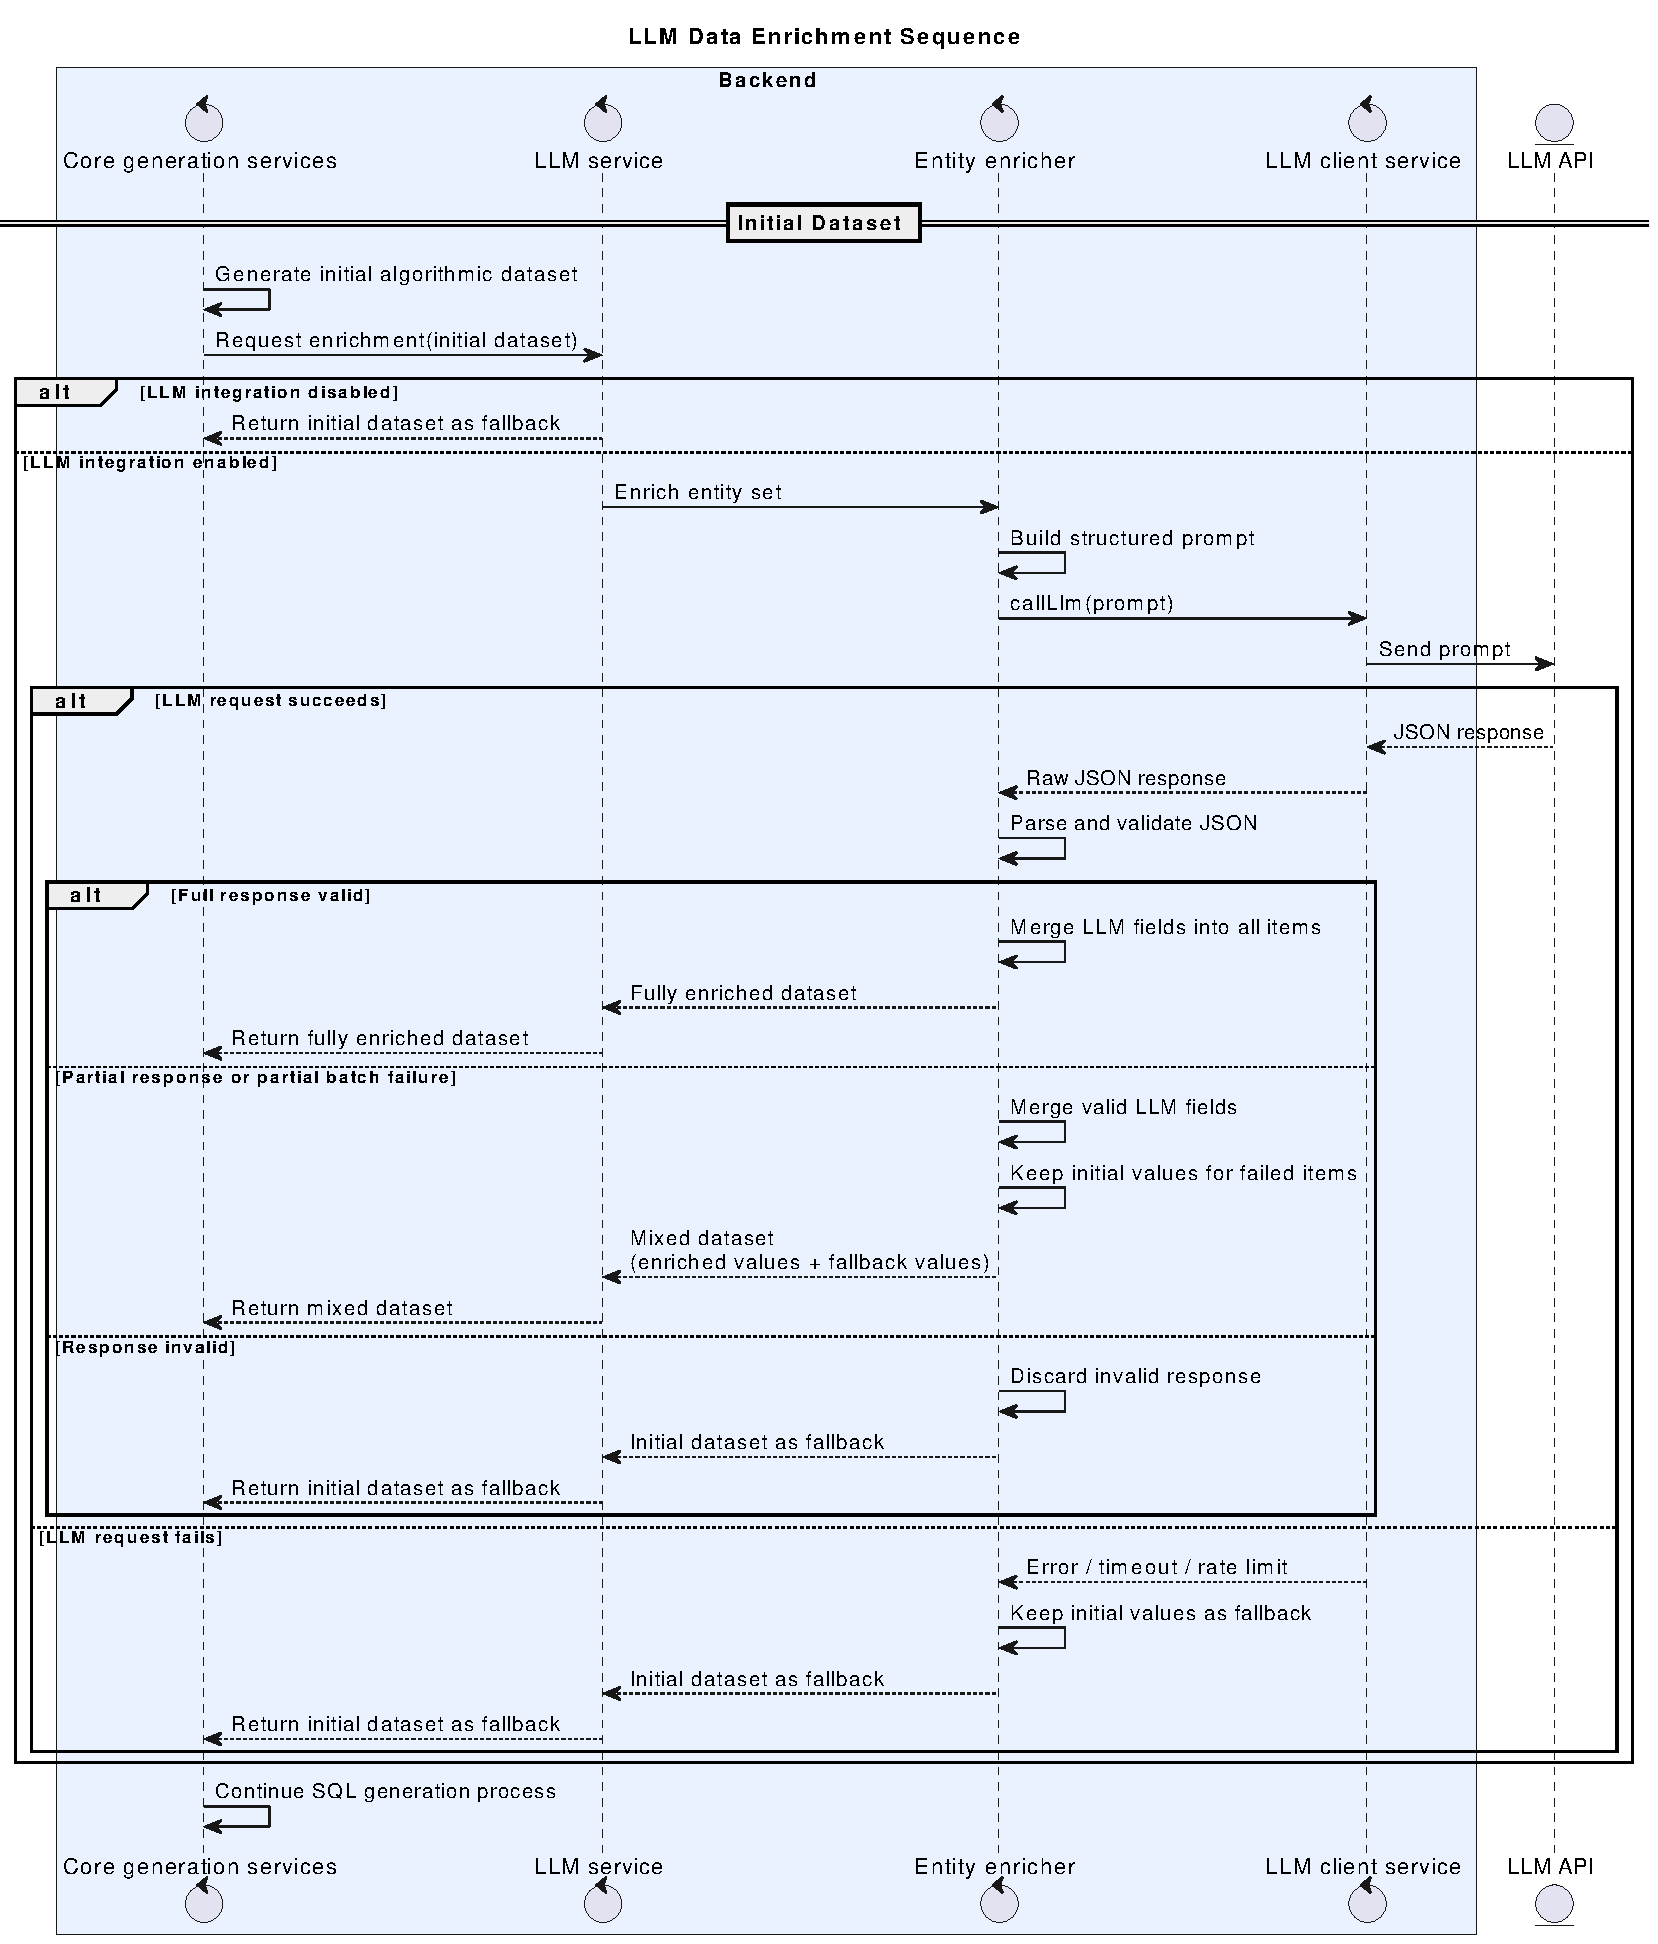
\includegraphics[width=0.95\textwidth]{img/sequence-llm-enrichment.pdf}
\caption{LLM enrichment sequence}
\label{fig:sequence-llm}
\end{figure}

\subsection{Class Diagram of Sprint 4}

\paragraph{}Figure~\ref{fig:sprint4-class-diagram} presents the main enrichment classes.

\begin{figure}[!htbp]
\centering
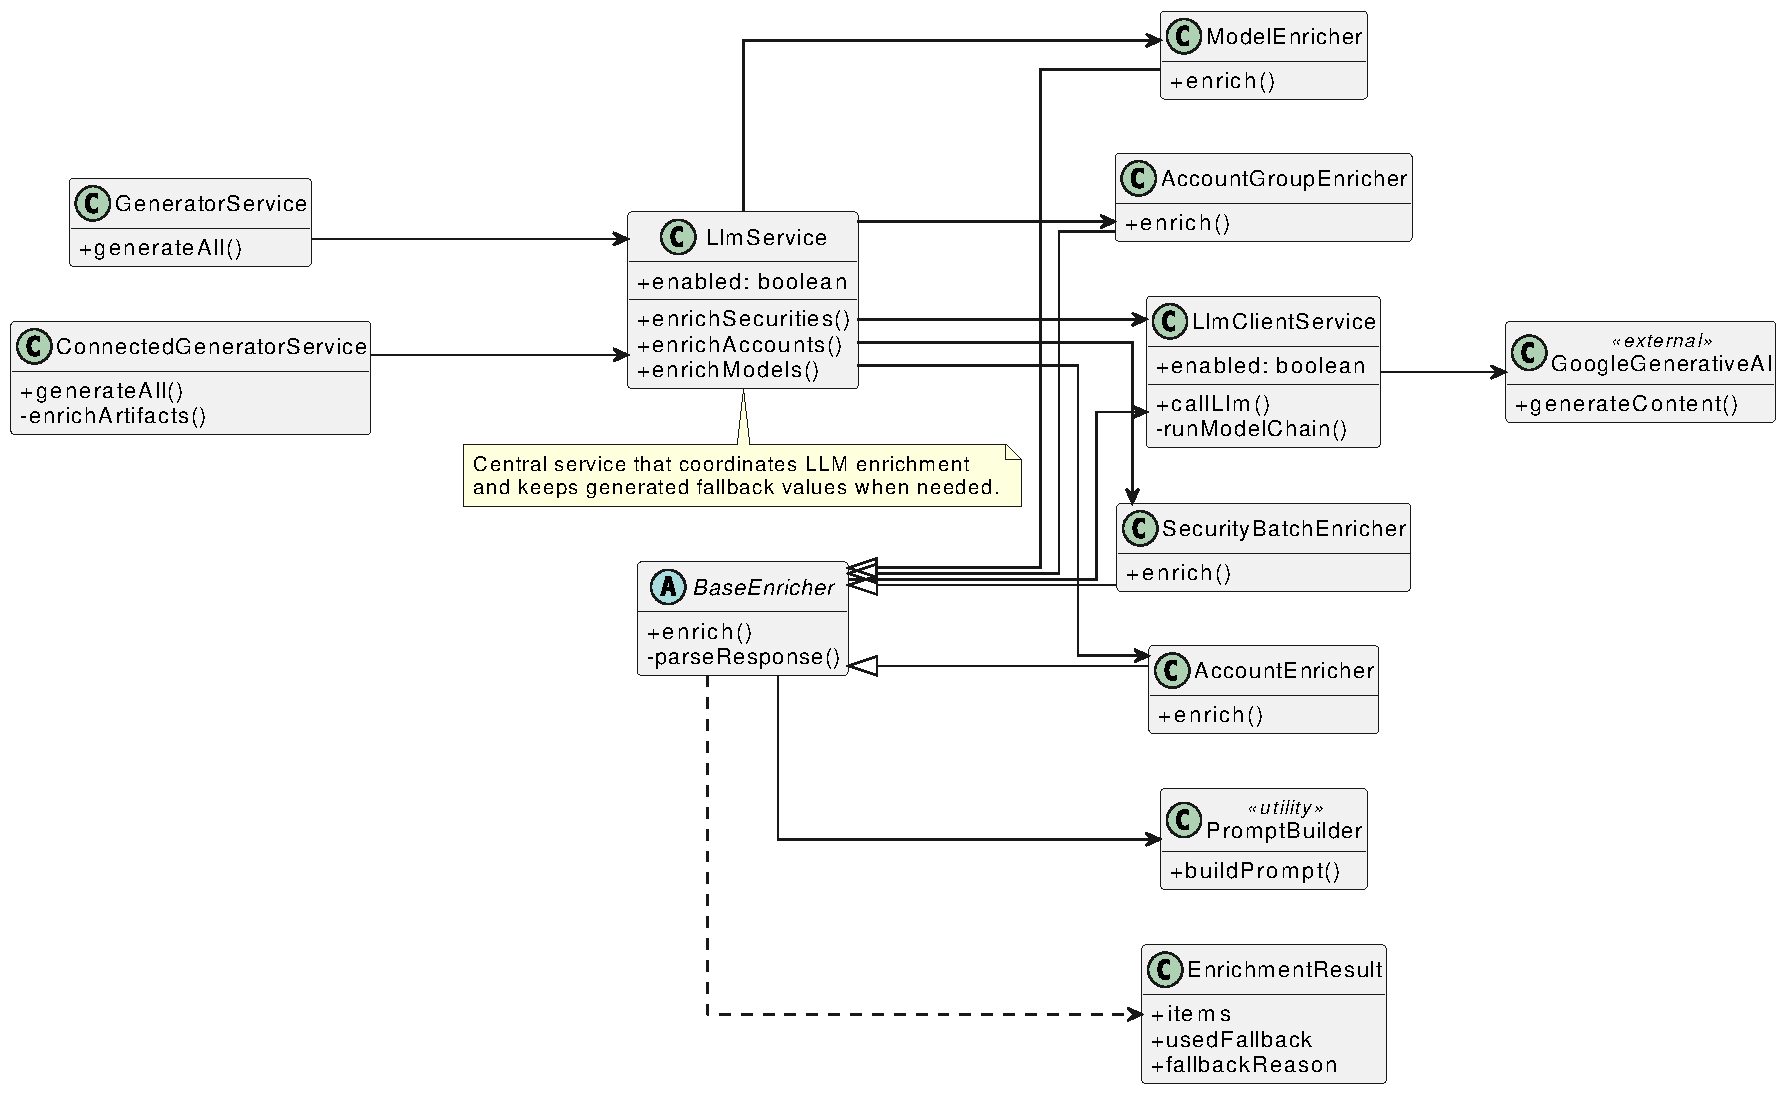
\includegraphics[width=0.95\textwidth]{img/llm-class-diagram.pdf}
\caption{Class diagram of Sprint 4}
\label{fig:sprint4-class-diagram}
\end{figure}

\subsection{LLM Provider Choice}

\paragraph{}Gemini was selected for this sprint because it offered a practical free-tier option during
development and provided enough quality for short financial text enrichment tasks. The objective was
not advanced reasoning, but fast generation of structured labels, symbols, and descriptions. For that
reason, the implementation uses Gemini 2.5 Flash as the preferred model and Gemini 2.5 Flash Lite as
the lighter fallback route before returning to algorithmic values.

\subsection{Prompt Engineering Strategy}

\paragraph{}Because the LLM receives only a controlled enrichment task, prompt engineering is centered
on structure and safety rather than open-ended generation. Table~\ref{tab:prompt-engineering-rules}
summarizes the rules used by the dedicated prompt builders.

\Needspace{11\baselineskip}
\renewcommand{\arraystretch}{1.25}
\begin{longtable}{|P{0.26\linewidth}|P{0.64\linewidth}|}
\caption{Prompt engineering rules used in Sprint 4}
\label{tab:prompt-engineering-rules} \\
\hline
\textbf{Rule} & \textbf{Implementation in the project} \\
\hline
\endfirsthead
\multicolumn{2}{r}{\tablename\ \thetable{} -- \textit{continued from previous page}} \\
\hline
\textbf{Rule} & \textbf{Implementation in the project} \\
\hline
\endhead
\hline
\multicolumn{2}{r}{\textit{continued on next page}} \\
\endfoot
\hline
\endlastfoot
Domain-specific prompts & Separate prompts are used for securities, accounts, account groups, and models. This avoids mixing unrelated instructions. \\
\hline
Business context & Prompts include useful context such as reference date, currencies, and the type of financial object to enrich. \\
\hline
JSON-only response & The LLM is instructed to return only a valid JSON array, without markdown, comments, explanations, or code fences. \\
\hline
Exact quantity control & The requested number of objects must match the number of objects returned by the LLM. If the count is wrong, fallback is used. \\
\hline
Identifier preservation & The LLM must copy backend-provided identifiers. This allows the enrichers to map each response to the correct generated record. \\
\hline
Allowed fields only & Each prompt lists only the fields that may be enriched, such as labels, names, symbols, or descriptions. Structural fields are never delegated to the LLM. \\
\hline
Response validation & The backend parses the JSON, checks expected IDs and types, applies maximum field lengths, and keeps deterministic values when the response is invalid. \\
\hline
\end{longtable}
\renewcommand{\arraystretch}{1}

\section{Realization}

\paragraph{}The backend implementation is located in \texttt{modules/llm}. Both standalone and connected
generation call \texttt{LlmService} after base records are created, then continue through the same
validation and output assembly steps used in the previous sprints.

\subsection{Internal Generation and LLM Enrichment Comparison}

\paragraph{}Table~\ref{tab:internal-vs-llm-comparison} shows why the LLM layer improves the
generator for QA work while the internal algorithm remains necessary for structure, volume, and
fallback.

\Needspace{13\baselineskip}
\renewcommand{\arraystretch}{1.3}
\begin{longtable}{|P{0.22\linewidth}|P{0.30\linewidth}|P{0.30\linewidth}|}
\caption{Comparison between internal generation and LLM-assisted enrichment}
\label{tab:internal-vs-llm-comparison} \\
\hline
\textbf{Criterion} & \textbf{Internal algorithm generation} & \textbf{LLM-assisted enrichment} \\
\hline
\endfirsthead
\multicolumn{3}{r}{\tablename\ \thetable{} -- \textit{continued from previous page}} \\
\hline
\textbf{Criterion} & \textbf{Internal algorithm generation} & \textbf{LLM-assisted enrichment} \\
\hline
\endhead
\hline
\multicolumn{3}{r}{\textit{continued on next page}} \\
\endfoot
\hline
\endlastfoot
Generation role & Produces valid rows, relationships, and loading order. & Improves only the readable fields after the valid dataset already exists. \\
\hline
Readability for QA & Technically valid, but names and labels can be generic or repetitive. & Produces clearer business-like names, labels, symbols, and descriptions. \\
\hline
Error detection & Harder to inspect in Longview when many records look similar. & Easier to recognize abnormal data because generated values look closer to real financial data. \\
\hline
Domain coherence & Applies fixed rules without understanding the business meaning of text fields. & Uses prompt context such as currencies, dates, entity type, and field constraints to create more coherent text. \\
\hline
Large data volumes & Best option for bulk generation and performance tests. & Used selectively because realistic enrichment is more useful for readable test sets than huge volume tests. \\
\hline
Safety & Deterministic and reproducible. & Safe because it cannot change IDs, quantities, prices, dates, relationships, or loading rules. \\
\hline
Final value & Guarantees that generation still works without external services. & Adds realism where it matters, with automatic fallback to the internal algorithm. \\
\hline
\end{longtable}
\renewcommand{\arraystretch}{1}

\subsection{API Key and Model Fallback Strategy}

\paragraph{}Figure~\ref{fig:llm-availability-fallback} shows the route used by the enrichment client. The
system first tries the two configured API keys with the preferred Gemini model, then with the lighter
fallback model. If no route returns a valid JSON response, deterministic values are kept.

\begin{figure}[!htbp]
\centering
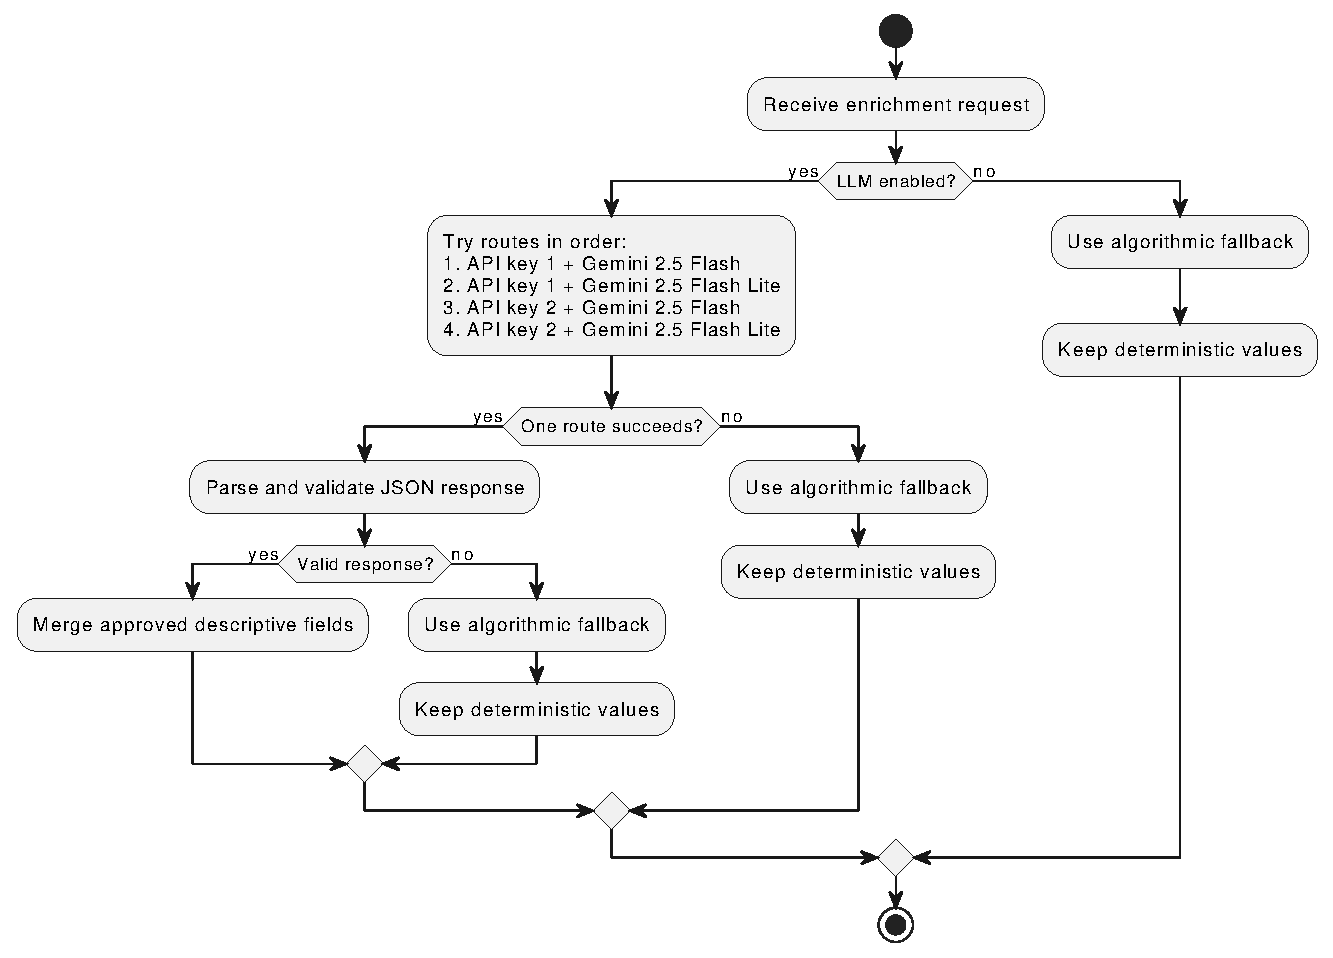
\includegraphics[width=0.82\textwidth]{img/llm-availability-fallback.pdf}
\caption{LLM availability and fallback mechanism}
\label{fig:llm-availability-fallback}
\end{figure}

\subsection{Implemented Components}

\renewcommand{\arraystretch}{1.15}
\begin{longtable}{|P{0.24\linewidth}|P{0.34\linewidth}|P{0.32\linewidth}|}
\caption{Main implemented LLM components}
\label{tab:llm-realization} \\
\hline
\textbf{Realized element} & \textbf{Project source} & \textbf{Role} \\
\hline
\endfirsthead
\multicolumn{3}{r}{\tablename\ \thetable{} -- \textit{continued from previous page}} \\
\hline
\textbf{Realized element} & \textbf{Project source} & \textbf{Role} \\
\hline
\endhead
\hline
\multicolumn{3}{r}{\textit{continued on next page}} \\
\endfoot
\hline
\endlastfoot
LLM facade & \texttt{llm.service.ts} & Coordinates enrichment for securities, accounts, groups, and models. \\
\hline
Provider client & \texttt{llm-client.service.ts} & Calls the AI provider and handles availability or parsing failures. \\
\hline
Security enrichment & \texttt{security-batch.enricher.ts} & Enriches multiple security subtypes with controlled textual values. \\
\hline
Account and group enrichment & \texttt{account.enricher.ts}, \texttt{account-group.enricher.ts} & Improves account labels while preserving account structure. \\
\hline
Model enrichment & \texttt{model.enricher.ts} & Improves model labels without changing allocation relationships. \\
\hline
Fallback behavior & \texttt{fallback-reason.util.ts} & Explains why deterministic values were kept when enrichment is unsafe. \\
\hline
\end{longtable}
\renewcommand{\arraystretch}{1}

\paragraph{}Figure~\ref{fig:ch6-llm-proof} is reserved as the realization proof for this sprint. It
should show an enriched generation result, a fallback log, or a before/after comparison of readable
fields produced by the LLM layer.

\begin{figure}[!htbp]
\centering
\IfFileExists{img/ch6-llm-proof.png}{%
    \includegraphics[width=0.88\textwidth]{img/ch6-llm-proof.png}%
}{%
    \fbox{\parbox[c][0.22\textheight][c]{0.86\textwidth}{\centering Screenshot to be added: LLM enrichment result, fallback log, or before/after enriched data comparison}}%
}
\caption{LLM enrichment output and fallback evidence}
\label{fig:ch6-llm-proof}
\end{figure}

\section*{Conclusion}
\addcontentsline{toc}{section}{Conclusion}

\paragraph{}Sprint 4 delivered controlled LLM enrichment for readable financial fields while preserving
the deterministic generation pipeline. The application can now improve labels, names, symbols, and
descriptions when the LLM is available, and keep algorithmic values when enrichment is unsafe,
unavailable, or unsuitable for large-volume tests.

        \clearpage
        
        \chapter*{Conclusion and perspectives}
\addcontentsline{toc}{chapter}{Conclusion and perspectives}
\markboth{Conclusion and perspectives}{}

\paragraph{}This final-year project focused on the design and implementation of a configurable test data
generator for Linedata Longview. The initial problem came from the difficulty of preparing coherent
test datasets manually for a financial platform whose data model contains many dependent entities:
accounts, account groups, hierarchies, models, securities, prices, positions, orders, and
executions. Manual SQL preparation was time-consuming, error-prone, difficult to reproduce, and
limited by confidentiality constraints that prevent the direct use of production data.

\paragraph{}The developed solution addresses this problem through a full-stack web application composed of a
React frontend and a NestJS backend. The system generates Longview-compatible pre-BCP records,
validates them, and assembles them into a SQL loading script that can be downloaded by QA engineers.
The standalone mode allows fully synthetic dataset
generation without a database connection, while the connected mode allows generated records to be
anchored to existing SQL Server accounts or securities selected by the user.

\paragraph{}The project was carried out using an Agile Scrum organization divided into five sprints. Sprint 1
mapped the Longview pre-BCP buffer model and established the population order. Sprint 2 delivered
the core generation engine and standalone workflow. Sprint 3 introduced SQL Server connectivity and
connected generation. Sprint 4 added optional LLM enrichment to improve the realism of descriptive
financial fields while preserving algorithmic fallback. Sprint 5 finalized the configuration
library, allowing users to save, load, rename, and delete reusable generation scenarios.

\paragraph{}Several engineering choices contributed to the reliability of the final tool. The generator was
implemented as a set of entity-specific services, making the business rules easier to isolate and
maintain. Validation is performed before file writing and SQL assembly, reducing the risk of
delivering invalid datasets. Connected mode uses read-only SQL queries and restricts raw table
fetching to approved Longview tables. LLM integration is optional and defensive: it enriches only
selected descriptive fields and never replaces deterministic generation as the source of structural
truth.

\paragraph{}The final application therefore meets the main objectives of the internship. It reduces manual
SQL preparation effort, improves reproducibility through saved configurations, supports both
standalone and connected test scenarios, and produces a coherent SQL script aligned with the
Longview loading process.

\paragraph{}Several perspectives remain possible for future work. The first improvement would be to extend
the generator to additional Longview entities and client-specific custom fields. A second direction
would be to add automated execution of the generated SQL script against a dedicated test database,
including a post-load verification report. A third perspective would be to introduce scenario
templates for common QA cases, such as full order lifecycle testing, fixed income schedule testing,
or derivative instrument testing. Finally, broader testing across multiple Longview environments
would help validate connected mode against different database configurations and client-specific
schema variations.

        \clearpage
        
        \printbibliography[heading=bibintoc]

    \backmatter
        %===== File containing the back cover of the document =====%

\thispagestyle{backcover}
\newgeometry{bottom=25mm,left=15mm,top=20mm,right=15mm}

\begin{changemargin}{3mm}{0cm}
    \begin{minipage}[c]{0.96\columnwidth}
        \selectlanguage{french}
        
        {\LARGE\textbf{Resume}}
        \vskip1mm
        \begingroup
            \large
            \@frenchAbstract
        \endgroup
        \vskip1mm
        {\textbf{Mots cles : }
            \begingroup
                \@frenchAbstractKeywords
            \endgroup
        }
        
        \vskip8mm
        \noindent\rule{\linewidth}{0.5pt}
        \vskip8mm
        
        \selectlanguage{english}
        {\LARGE\textbf{Abstract}}
        \vskip1mm
        \begingroup
            \large
            \@englishAbstract
        \endgroup
        \vskip1mm
        {\textbf{Keywords : }
            \begingroup
                \@englishAbstractKeywords
            \endgroup
        }
    \end{minipage}
\end{changemargin}

        \clearpage

\end{document}